\chapter{Results and User Interface}

\section{Introduction}

This chapter presents the implementation results of the proposed Smart Placement Preparation Platform (PrepSmart) through the developed user interfaces. The screenshots included in this chapter demonstrate the major functionalities implemented during the development of the system and illustrate how users interact with different modules of the application.

The platform provides a modern and intuitive web interface that enables students to access placement preparation resources through a single integrated application. The implemented modules include user authentication, personalized dashboards, structured learning paths, coding practice, mock assessments, AI-assisted interview preparation, company-specific readiness analysis, portfolio management, skills passport generation, analytics, and administrative tools.

Each section of this chapter presents the corresponding user interface along with a detailed explanation of its functionality, highlighting how the developed system addresses the challenges identified during the requirement analysis phase.

\section{Landing Page}

The landing page serves as the public entry point of the PrepSmart platform. It introduces visitors to the objectives, major features, and capabilities of the application before authentication. The page is designed to provide a professional first impression while allowing users to easily navigate to the registration or login pages.

The interface follows a clean and responsive design, ensuring compatibility across different screen sizes and devices. Important features of the platform are highlighted using descriptive sections and interactive components, enabling prospective users to understand the purpose of the system before creating an account.

\begin{figure}[H]
\centering
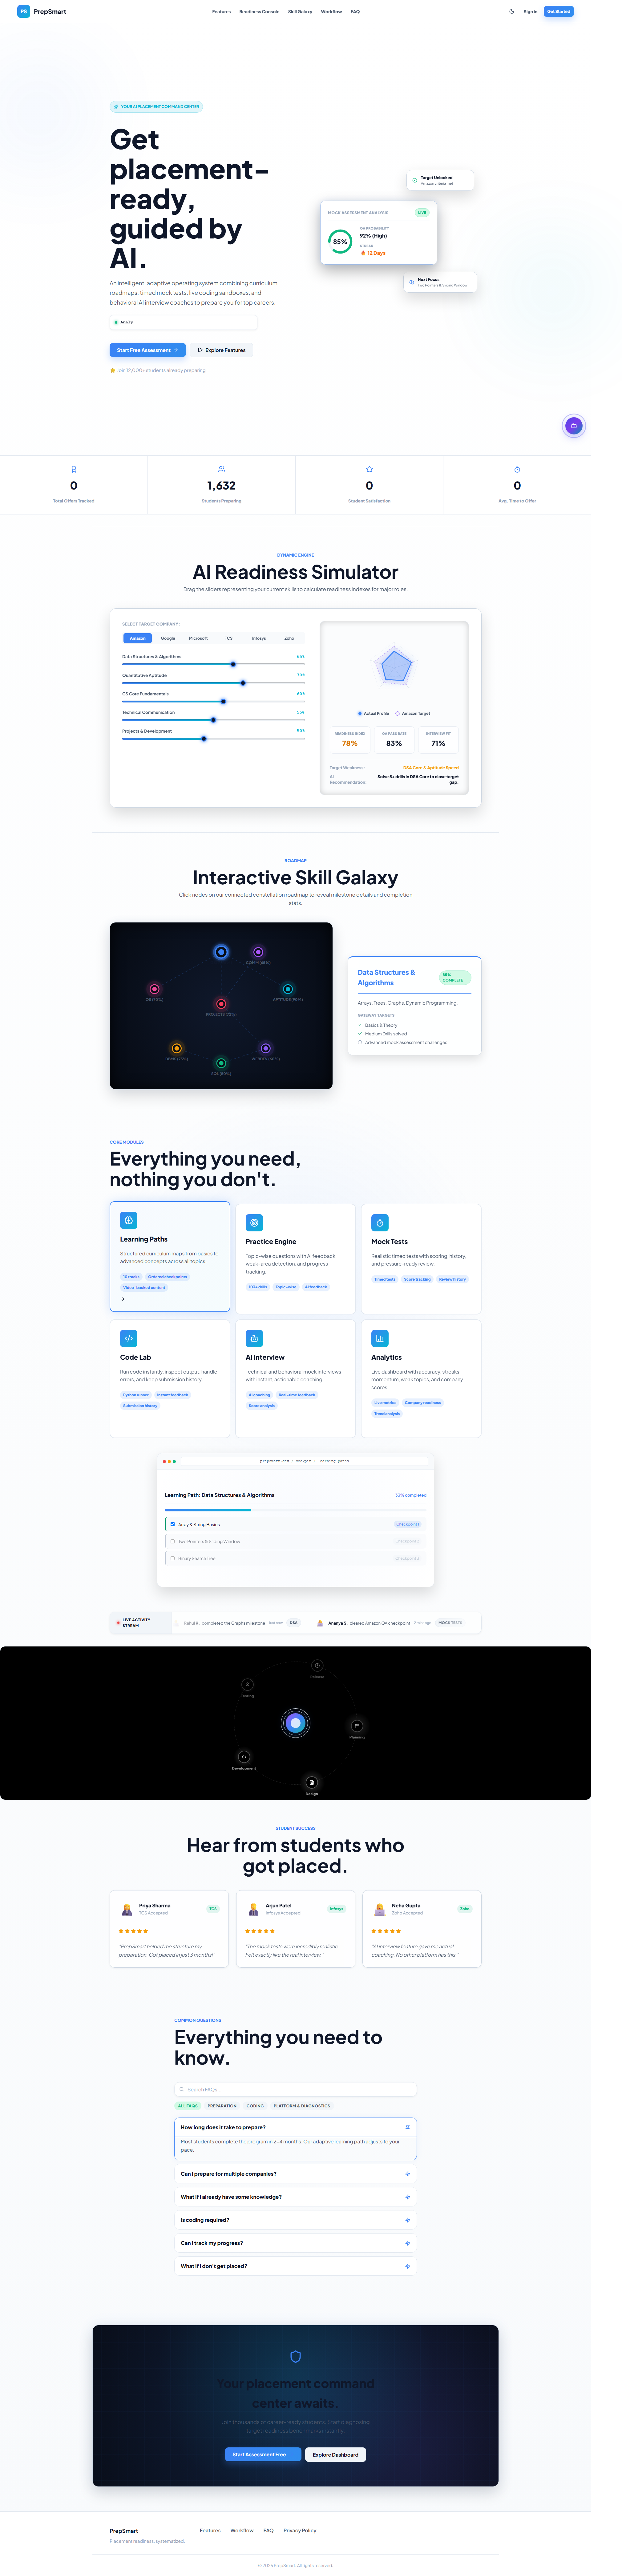
\includegraphics[width=0.70\textwidth]{Media/Chapter 5/landing.png}
\caption{Landing Page of PrepSmart}
\label{fig:landing_page}
\end{figure}

Figure~\ref{fig:landing_page} illustrates the landing page presented to users when they access the PrepSmart platform. The homepage introduces the application and highlights its primary objective of providing a unified environment for placement preparation.

The navigation menu provides quick access to important sections of the application, while prominent action buttons allow users to register for a new account or log into an existing account. The landing page also presents the core features offered by the platform, including structured learning paths, coding practice, mock tests, AI-powered interview preparation, company readiness tracking, portfolio generation, and performance analytics.

The responsive layout ensures consistent presentation across desktop and mobile devices. Visual elements, icons, and feature cards improve usability and make the interface easy to understand for first-time users. Overall, the landing page serves as the gateway to the platform and effectively communicates the functionality and benefits of PrepSmart.

\subsection{Major Features of the Landing Page}

The landing page provides the following features:

\begin{itemize}

\item Introduction to the PrepSmart platform.

\item Navigation to login and registration pages.

\item Overview of the major placement preparation modules.

\item Responsive and user-friendly interface.

\item Professional presentation of platform capabilities.

\item Quick access to important information for new users.

\end{itemize}

\subsection{Advantages}

The landing page offers several advantages:

\begin{itemize}

\item Creates a professional first impression.

\item Clearly communicates the purpose of the platform.

\item Simplifies navigation for new users.

\item Highlights the major features available after authentication.

\item Provides a responsive interface for different devices.

\end{itemize}

\section{User Authentication}

User authentication is the first step in accessing the personalized features of the PrepSmart platform. The authentication module ensures that only registered users can access protected resources such as dashboards, learning modules, coding practice, AI interviews, company readiness tracking, and profile management.

The platform provides separate interfaces for user login and new user registration. Both interfaces are designed to be simple, responsive, and user-friendly while ensuring secure authentication using JSON Web Tokens (JWT).

\subsection{Login Page}

The login page allows registered users to securely access the PrepSmart platform by verifying their credentials. The interface is designed to provide a simple and intuitive authentication experience while maintaining application security.

\begin{figure}[H]
\centering
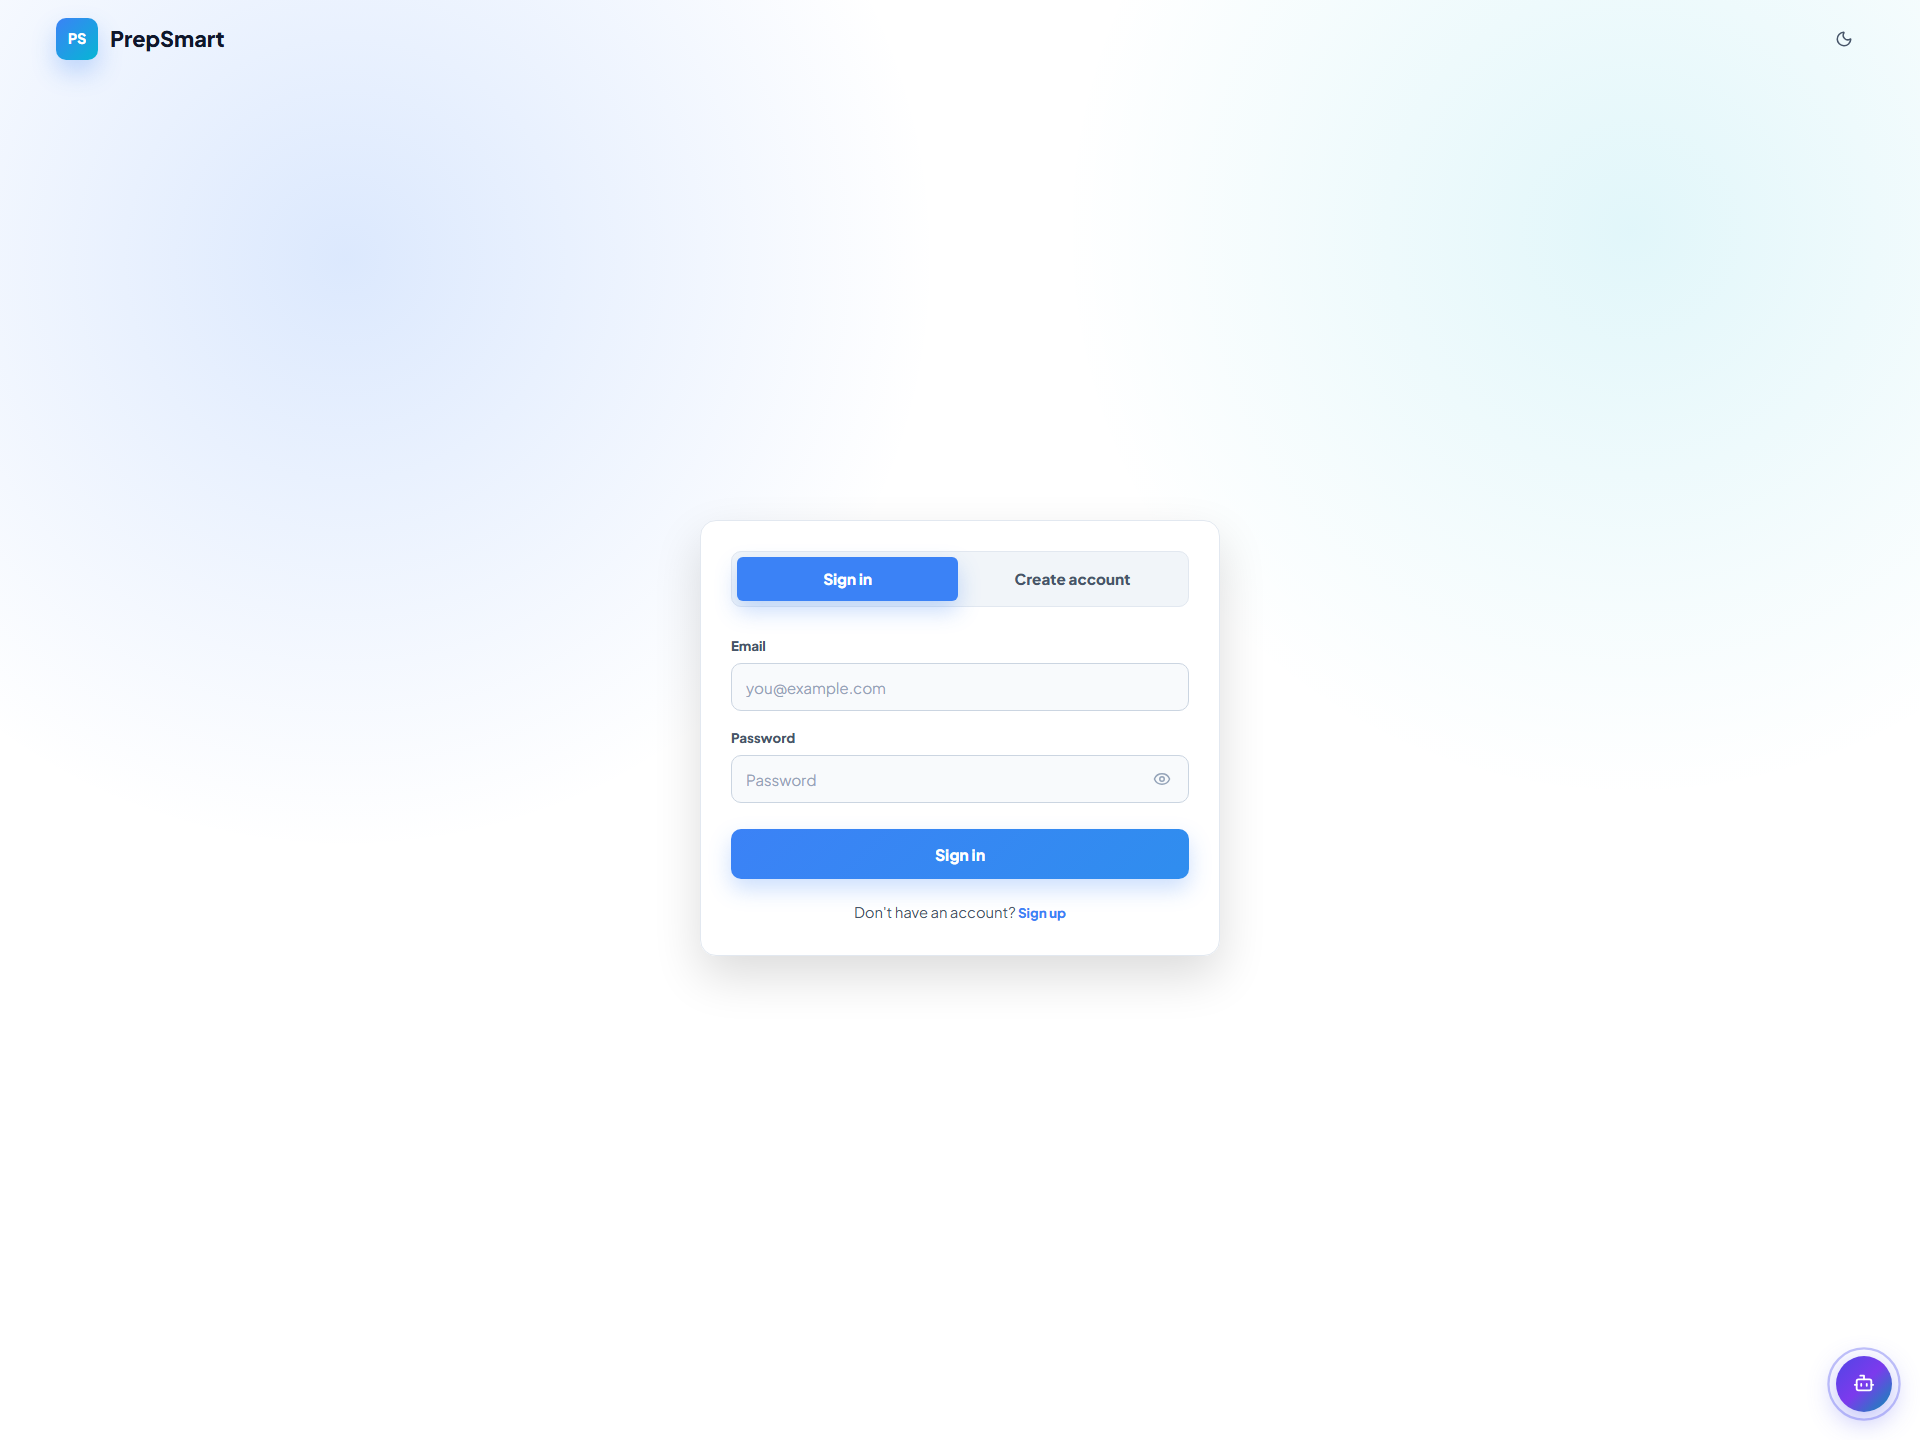
\includegraphics[width=\textwidth]{Media/Chapter 5/login.png}
\caption{Login Page}
\label{fig:login_page}
\end{figure}

Figure~\ref{fig:login_page} shows the login interface of PrepSmart. Registered users enter their email address and password to authenticate themselves before accessing the platform. After successful authentication, the system generates a JSON Web Token (JWT) and redirects the user to the personalized dashboard.

The login interface includes input fields for user credentials along with validation mechanisms that prevent invalid or incomplete submissions. Appropriate error messages are displayed whenever incorrect credentials are entered, enabling users to correct their information before attempting to log in again.

The interface follows a clean and responsive design that ensures consistent usability across different devices. Once authenticated, users gain access to all modules associated with their account, including placement preparation, coding practice, AI interview sessions, portfolio management, and analytics.

\subsubsection*{Major Features}

\begin{itemize}

\item Secure user authentication.

\item Email and password validation.

\item JWT-based session management.

\item Error handling for invalid credentials.

\item Responsive and user-friendly interface.

\item Direct navigation to the dashboard after successful login.

\end{itemize}

\subsection{Registration Page}

The registration page enables new users to create an account on the PrepSmart platform. The interface collects the required personal and academic information before securely creating a new user profile.

\begin{figure}[H]
\centering
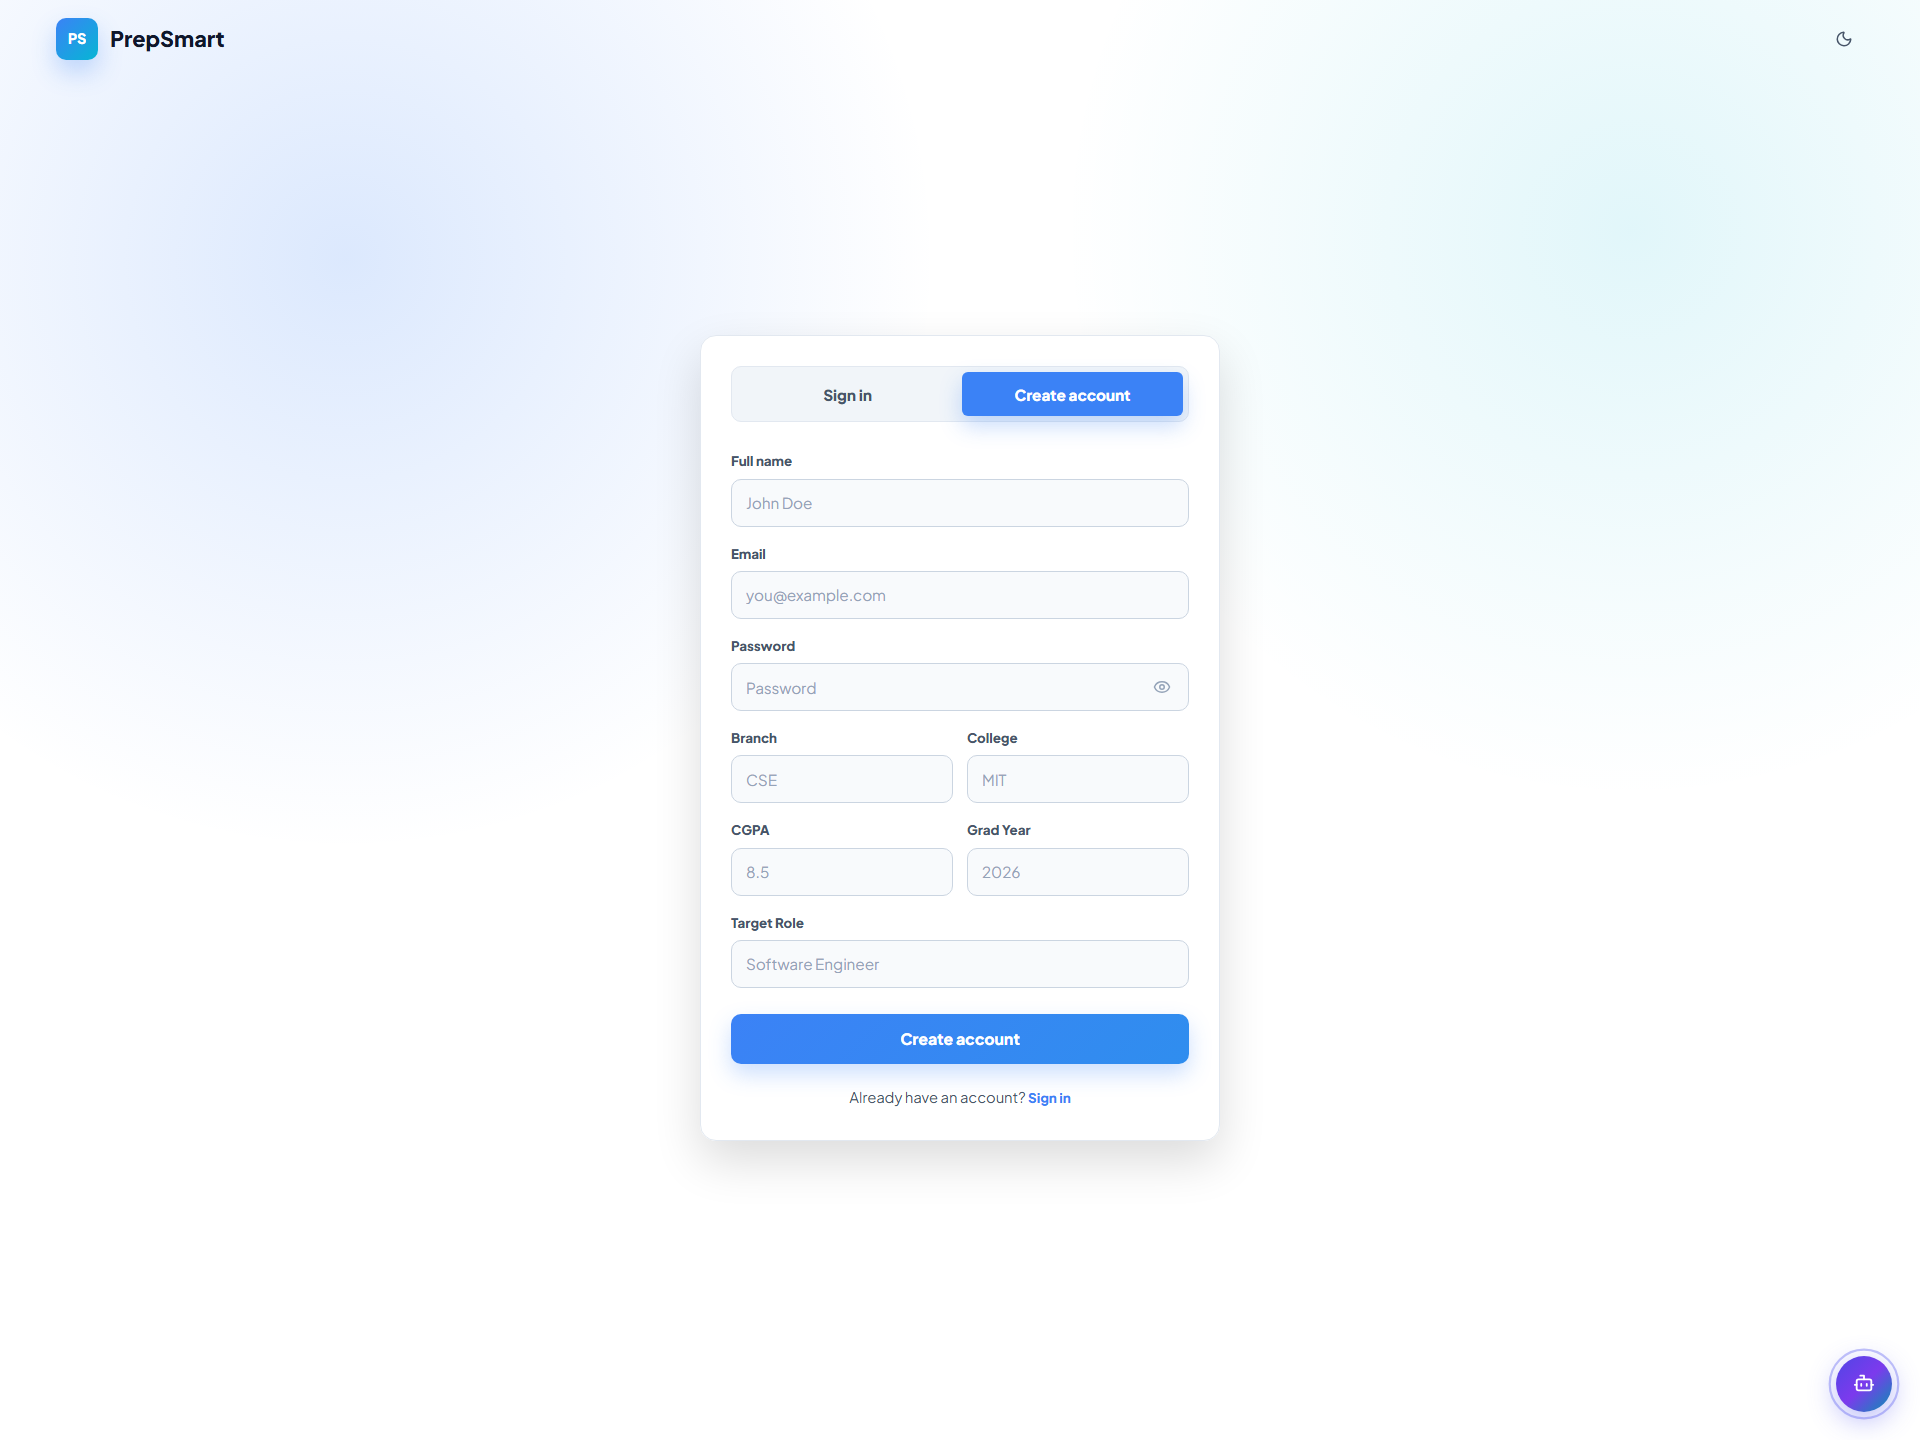
\includegraphics[width=\textwidth]{Media/Chapter 5/signup.png}
\caption{User Registration Page}
\label{fig:signup_page}
\end{figure}

Figure~\ref{fig:signup_page} illustrates the user registration interface of PrepSmart. New users provide the required information such as name, email address, password, and other registration details to create an account.

Before creating the account, the backend validates the submitted information to ensure that mandatory fields are completed correctly and that duplicate accounts are not created. Upon successful registration, a new user profile is generated and stored in the database.

The registration interface is designed to minimize complexity while providing sufficient validation to maintain data integrity. Once registration is completed successfully, users can log into the platform using their newly created credentials and begin their placement preparation journey.

\subsubsection*{Major Features}

\begin{itemize}

\item New user registration.

\item Input validation.

\item Duplicate account prevention.

\item Secure password handling.

\item Automatic user profile creation.

\item Integration with JWT authentication.

\end{itemize}

\section{Dashboard}

The Dashboard serves as the central workspace of the PrepSmart platform. After successful authentication, users are redirected to this page, where they can monitor their overall placement preparation progress through a unified and interactive interface. The dashboard consolidates information from multiple modules, including learning progress, coding practice, mock tests, interview preparation, company readiness, and daily goals.

The dashboard is designed to provide students with an overview of their current preparation status, helping them identify completed activities, pending tasks, and areas requiring improvement. Instead of navigating through multiple pages, users can quickly access the most important information from a single interface.

\begin{figure}[H]
\centering
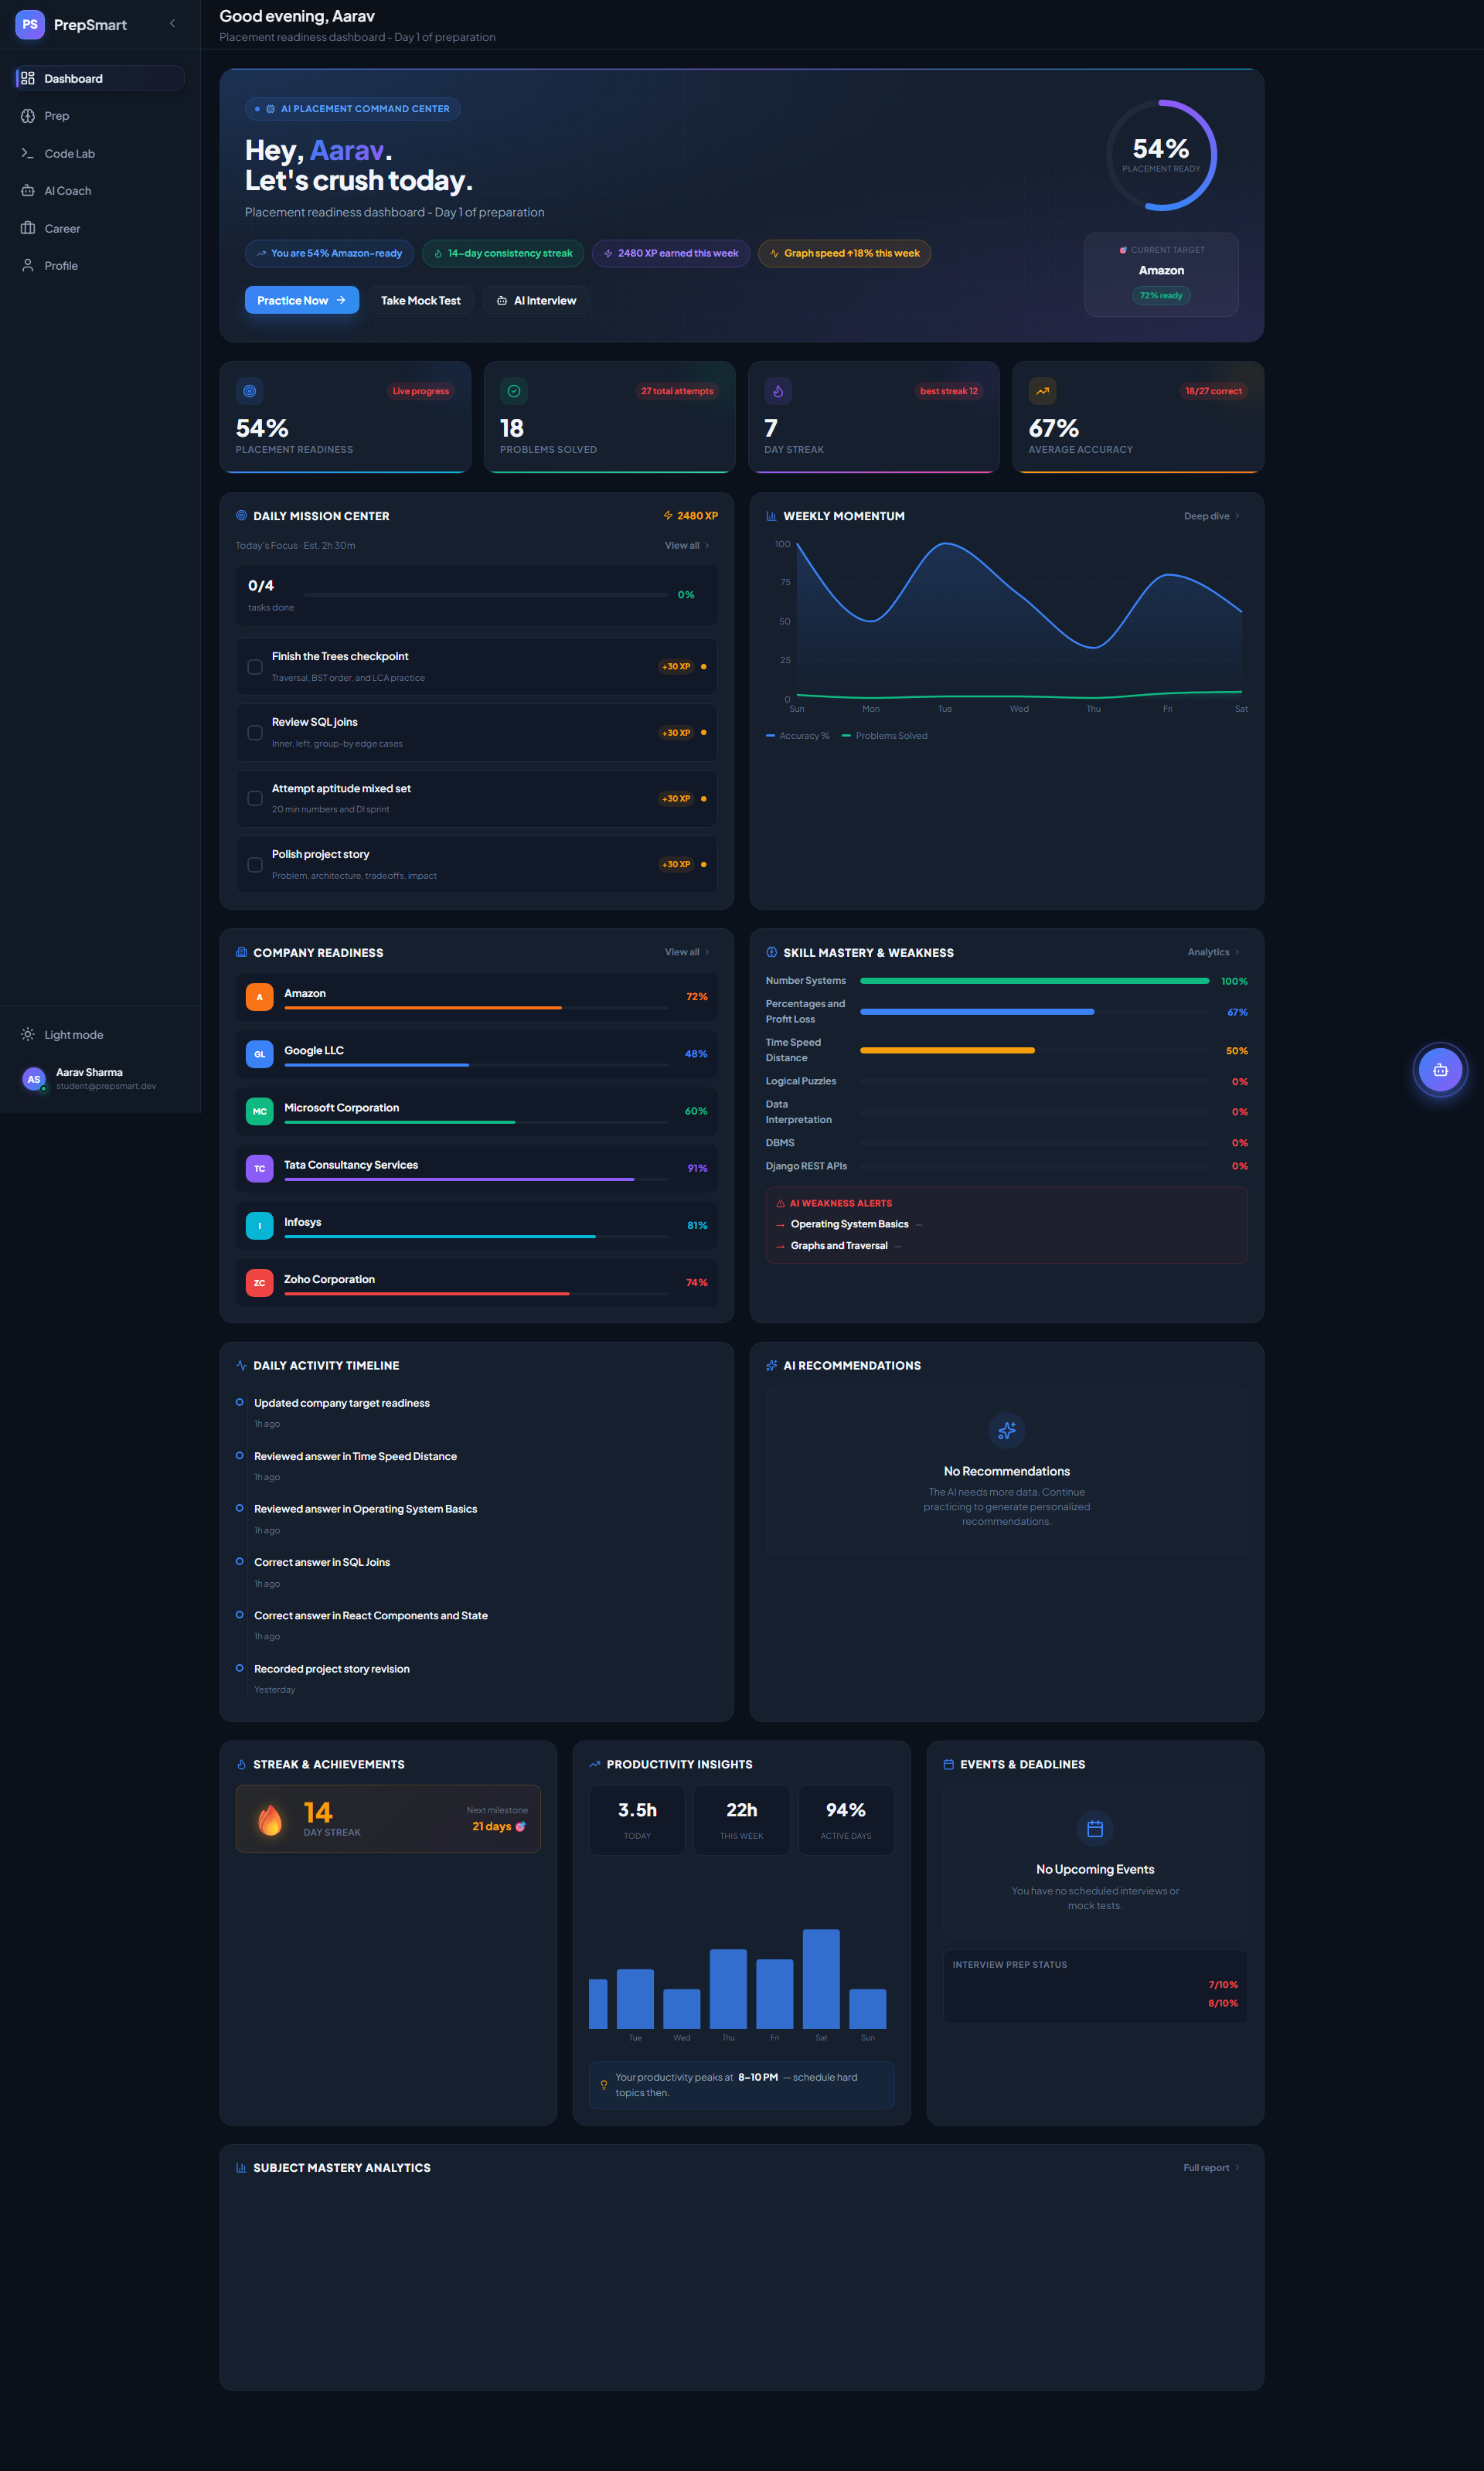
\includegraphics[width=0.95\textwidth]{Media/Chapter 5/dashboard.png}
\caption{Student Dashboard}
\label{fig:dashboard}
\end{figure}

Figure~\ref{fig:dashboard} illustrates the main dashboard of the PrepSmart platform. After authentication, this page acts as the personalized homepage for every student. The dashboard aggregates information from different modules and presents it in an organized manner using cards, charts, progress indicators, and statistical summaries.

The upper section of the dashboard displays important performance metrics such as placement readiness, completed topics, coding activity, interview progress, and overall learning statistics. These indicators are updated automatically whenever the student completes learning activities, coding problems, mock tests, or interview sessions.

The central portion of the dashboard provides quick access to active learning tracks, daily goals, recent activities, recommended topics, and upcoming preparation milestones. This allows students to continue their preparation without manually searching for unfinished tasks.

The dashboard also includes visual analytics that summarize preparation progress using graphs and progress bars. These visualizations help students understand their strengths and weaknesses while enabling continuous monitoring of their placement readiness. Since all information is retrieved dynamically from the backend database, the dashboard always reflects the latest progress of the student.

\subsection{Major Components of the Dashboard}

The dashboard consists of several important components that assist students during placement preparation.

\begin{itemize}

\item Personalized welcome section.

\item Overall placement readiness score.

\item Learning progress indicators.

\item Coding practice statistics.

\item Mock test performance summary.

\item AI interview readiness information.

\item Daily learning goals.

\item Activity history.

\item Recommended learning tasks.

\item Navigation shortcuts to major modules.

\end{itemize}

\subsection{Functionalities}

The Dashboard provides the following functionalities:

\begin{itemize}

\item Displays real-time preparation statistics.

\item Tracks completion of learning topics.

\item Shows coding practice performance.

\item Monitors interview readiness.

\item Displays company preparation status.

\item Provides personalized recommendations.

\item Enables quick navigation to learning modules.

\item Updates automatically after every completed activity.

\end{itemize}

\subsection{Advantages}

The Dashboard offers several advantages to students preparing for campus placements.

\begin{itemize}

\item Centralized view of placement preparation.

\item Real-time progress monitoring.

\item Easy identification of weak areas.

\item Better learning organization.

\item Improved motivation through progress visualization.

\item Efficient access to all major platform modules.

\end{itemize}

\section{Placement Preparation Module}

The Placement Preparation Module is the primary learning component of PrepSmart. It provides students with a structured and organized approach towards campus placement preparation by combining learning paths, milestone tracking, topic-wise study materials, and continuous progress monitoring within a single platform.

Unlike traditional preparation methods that require students to use multiple websites, this module integrates all essential learning resources into one environment. Students can systematically complete learning tracks, monitor their progress, and prepare for technical interviews in a guided manner.

The module consists of four major interfaces: Prep Journey, Learning Roadmaps, Milestones, and Topic Study. Each interface contributes to different stages of the student's preparation process.

\subsection{Prep Journey}

The Prep Journey interface provides students with a personalized learning roadmap that organizes placement preparation into structured tracks and learning stages. It enables users to monitor completed topics, pending activities, and overall preparation progress.

\begin{figure}[H]
\centering
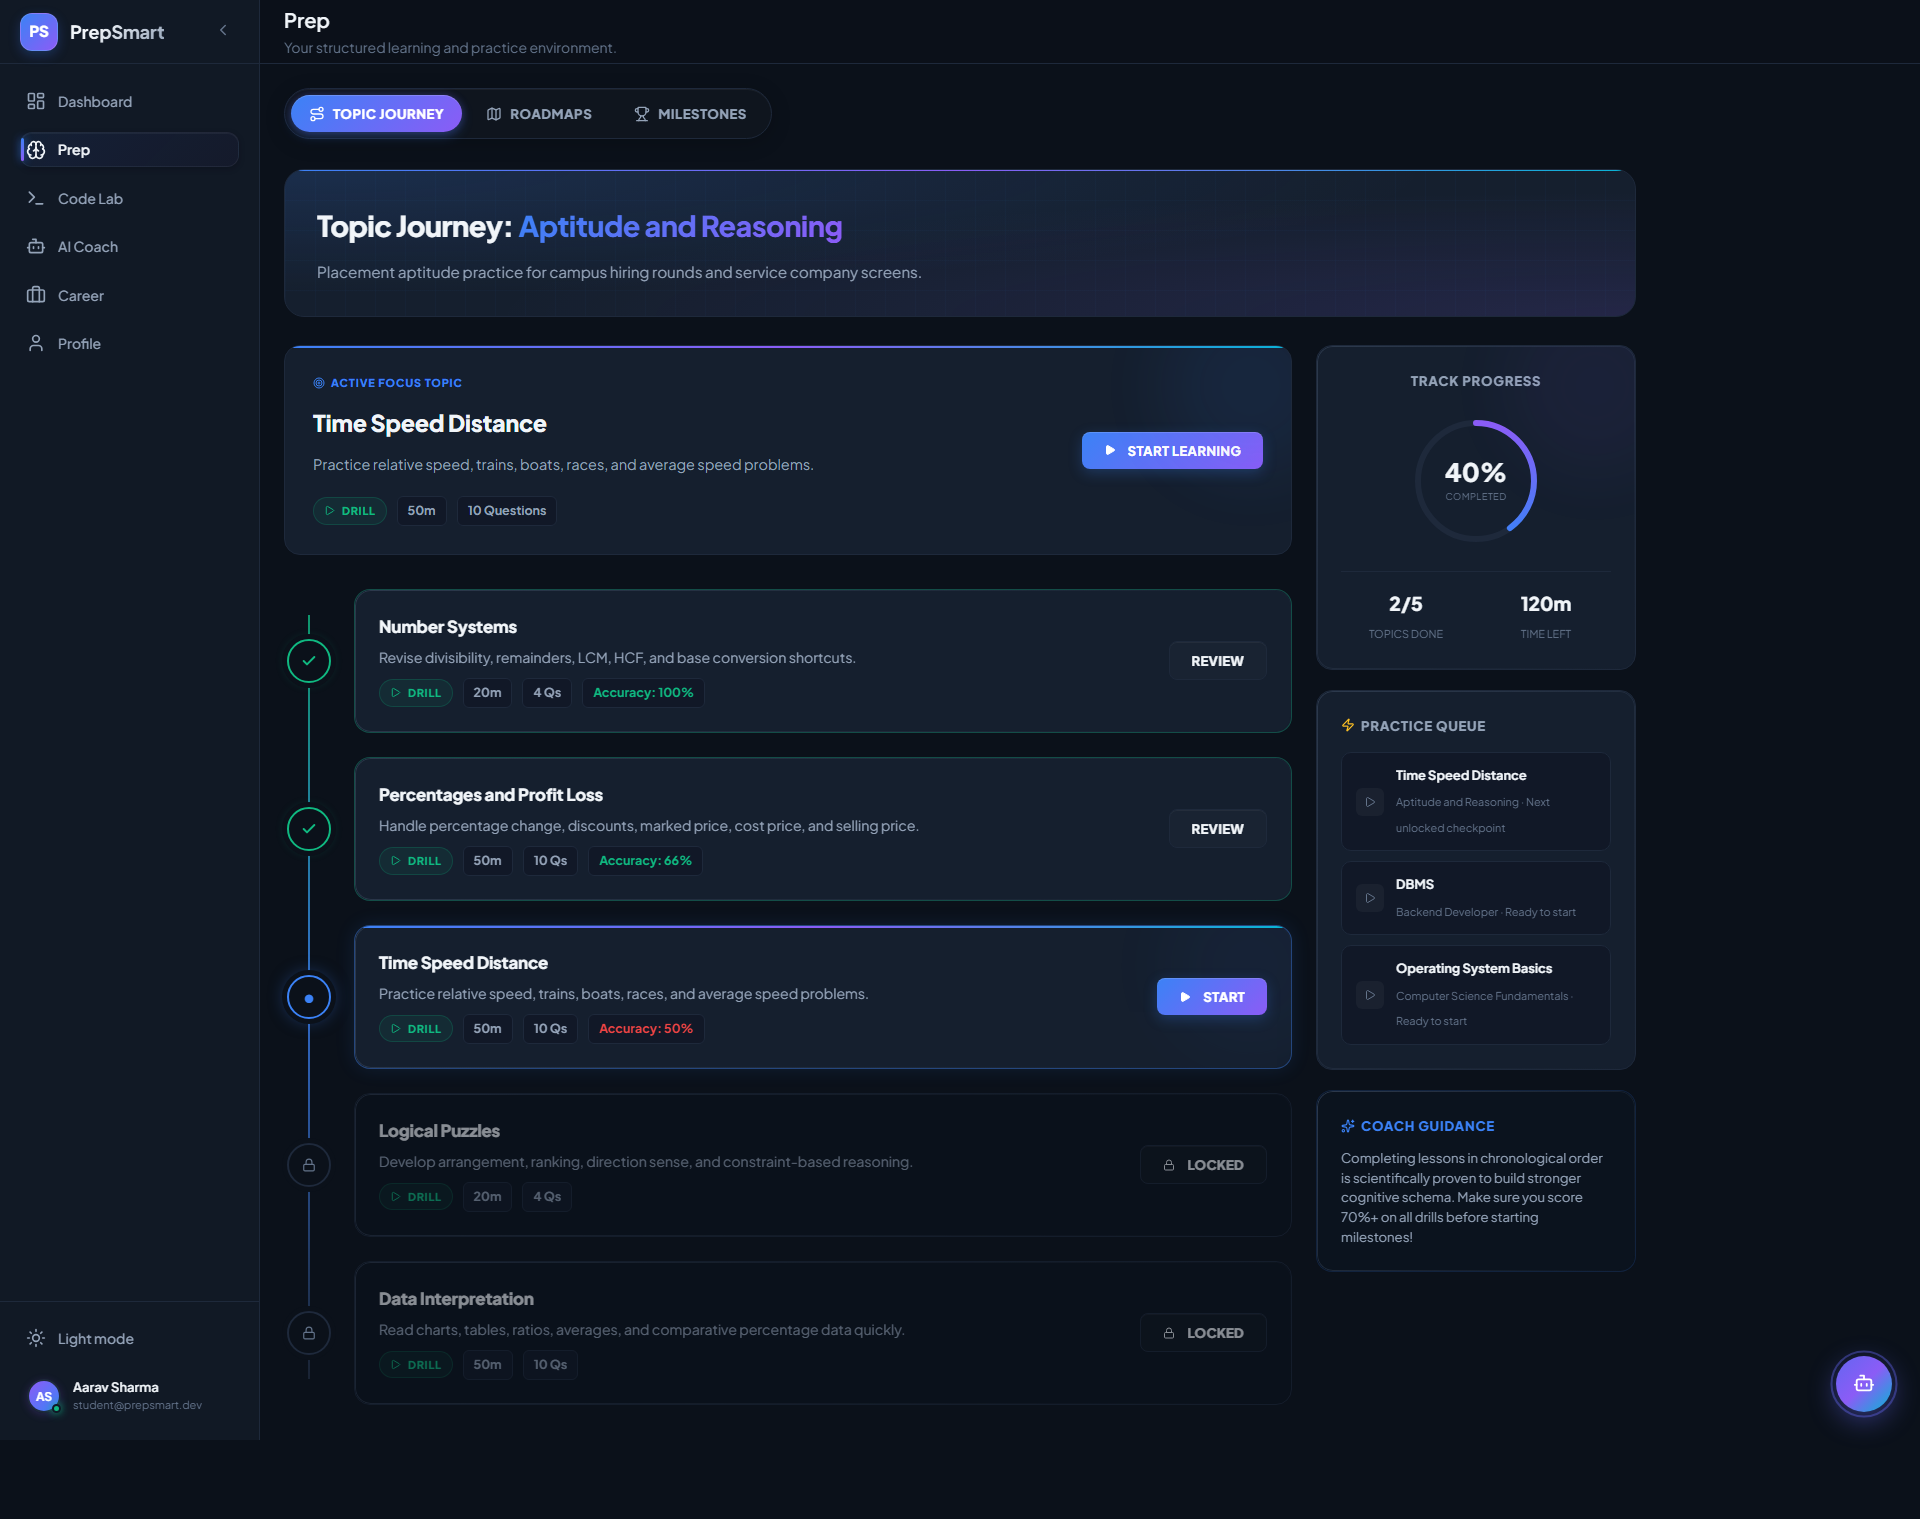
\includegraphics[width=0.95\textwidth]{Media/Chapter 5/prep_journey.png}
\caption{Prep Journey Interface}
\label{fig:prep_journey}
\end{figure}

Figure~\ref{fig:prep_journey} illustrates the Prep Journey interface of PrepSmart. This page acts as the student's personalized learning roadmap by presenting different preparation tracks in a well-organized manner.

Each learning track contains multiple topics arranged according to their recommended learning sequence. As students complete individual topics and assessments, their progress is automatically updated and reflected within the interface. This enables users to clearly distinguish between completed topics, ongoing learning activities, and pending preparation tasks.

The interface also recommends the next learning objective based on the student's previous progress, allowing users to follow a continuous and systematic preparation strategy without manually planning their studies.

\subsubsection*{Major Features}

\begin{itemize}

\item Structured learning tracks.

\item Topic completion tracking.

\item Progress visualization.

\item Personalized learning recommendations.

\item Automatic learning sequence management.

\item Integration with dashboard analytics.

\end{itemize}

\subsection{Learning Roadmaps}

The Learning Roadmaps interface presents detailed preparation paths for various placement domains. Each roadmap guides students through the recommended order of topics required to develop strong technical knowledge before attending placement interviews.

\begin{figure}[H]
\centering
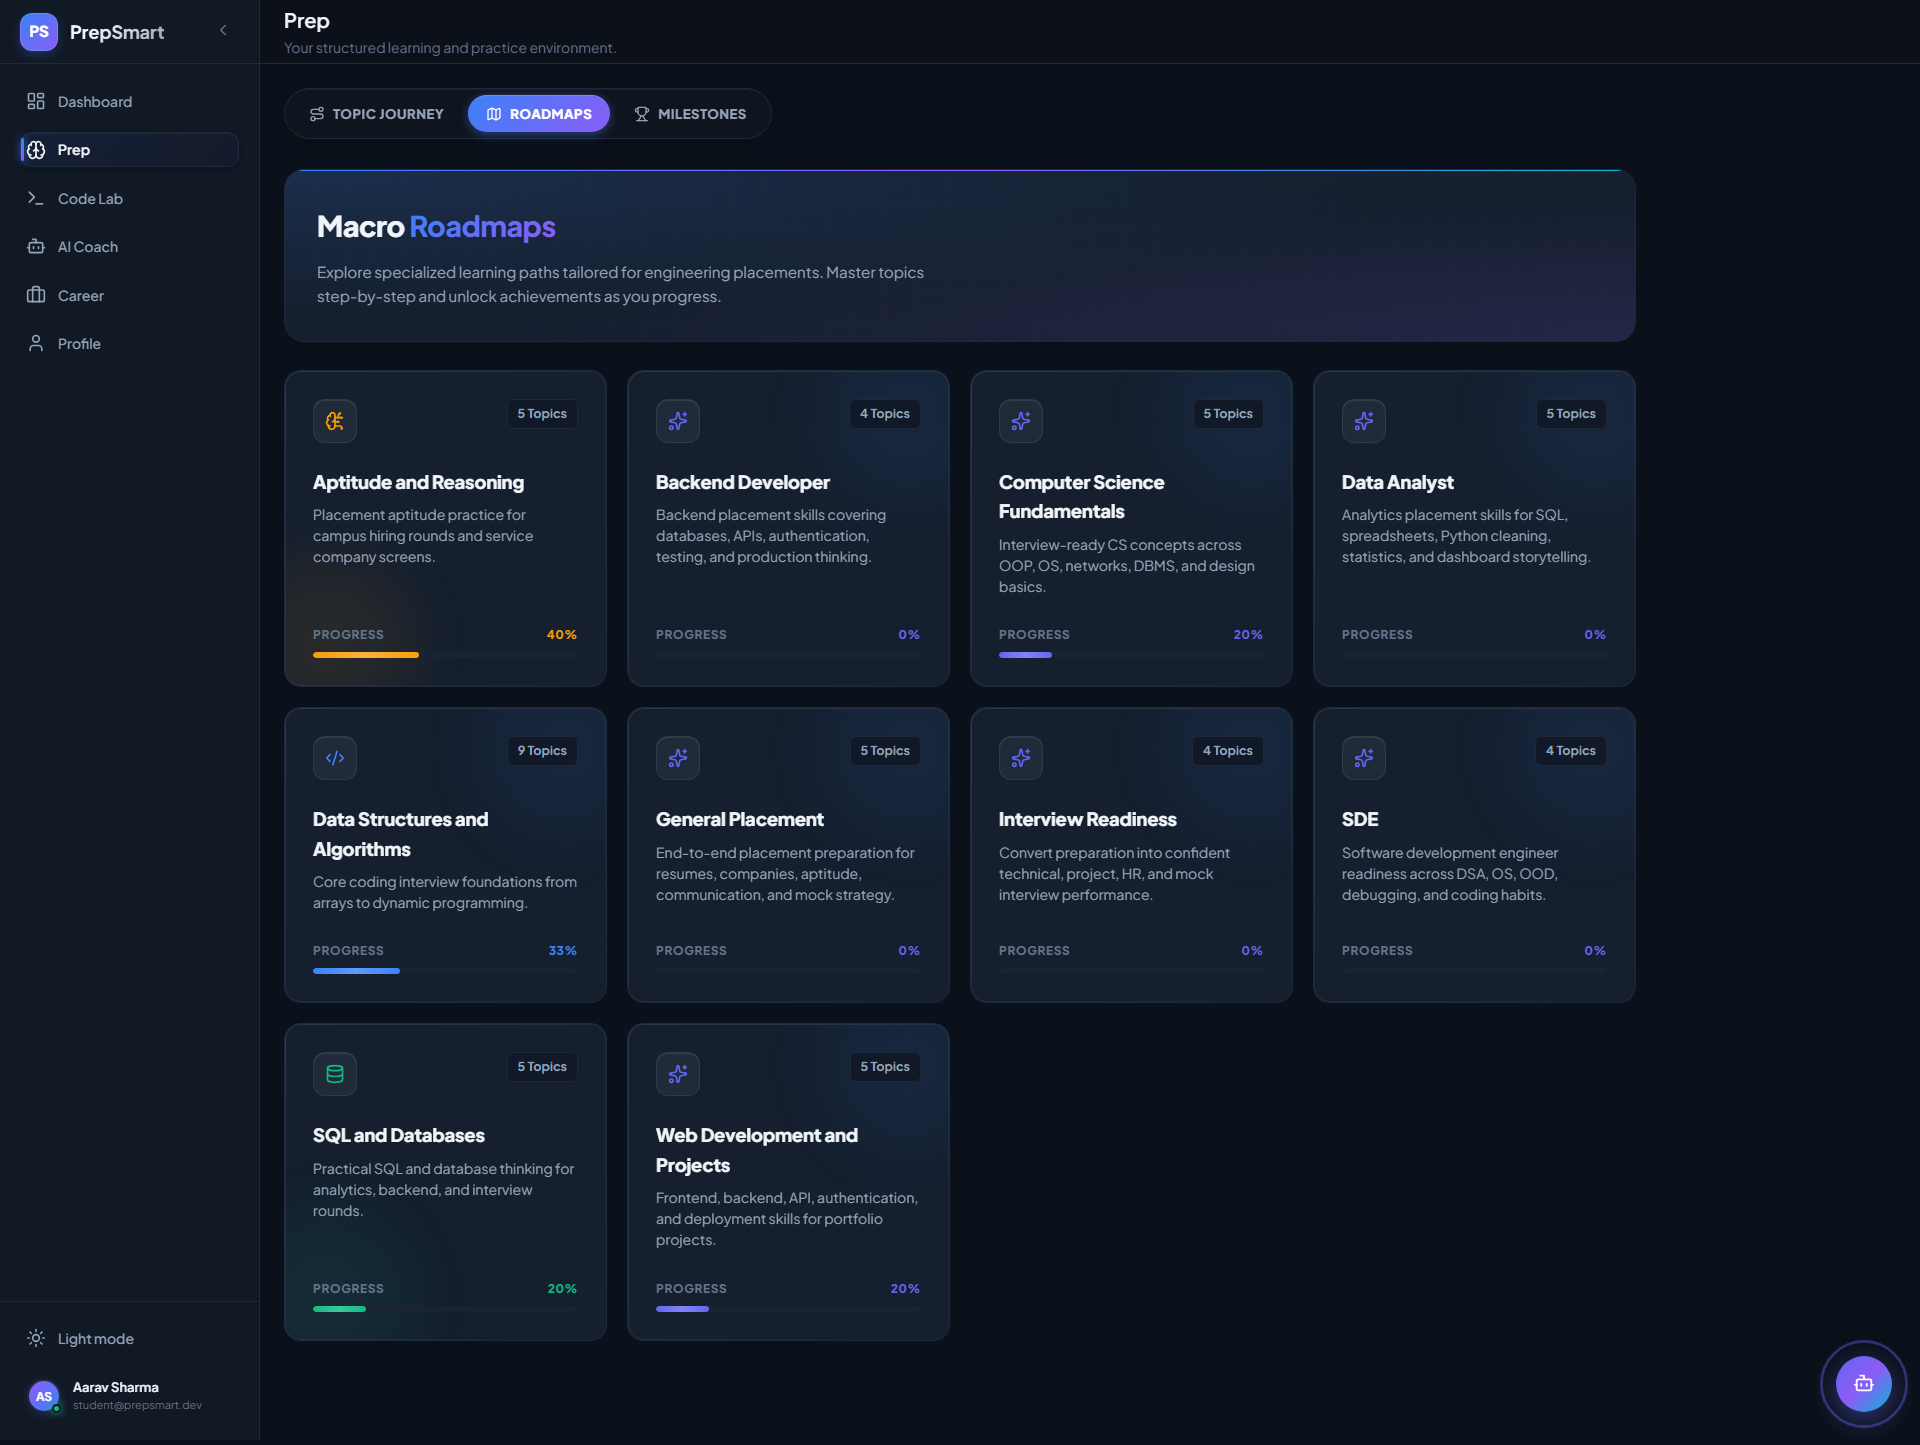
\includegraphics[width=0.95\textwidth]{Media/Chapter 5/roadmaps.png}
\caption{Learning Roadmaps}
\label{fig:learning_roadmaps}
\end{figure}

Figure~\ref{fig:learning_roadmaps} presents the Learning Roadmaps available within PrepSmart. The page organizes learning content into multiple preparation paths, allowing students to focus on specific technical domains based on their placement goals.

Each roadmap contains an ordered sequence of learning topics designed to gradually increase the student's understanding from fundamental concepts to advanced interview-level knowledge. Students can select individual roadmaps according to their interests and preparation requirements.

The roadmap interface simplifies long-term planning by clearly indicating learning dependencies and recommended study sequences.

\subsubsection*{Major Features}

\begin{itemize}

\item Domain-specific learning paths.

\item Sequential topic organization.

\item Guided placement preparation.

\item Easy roadmap navigation.

\item Progress monitoring.

\item Future learning recommendations.

\end{itemize}

\subsection{Milestones}

The Milestones interface enables students to evaluate their preparation by completing predefined learning checkpoints. These milestones divide the preparation journey into manageable stages, allowing continuous assessment of learning progress.

\begin{figure}[H]
\centering
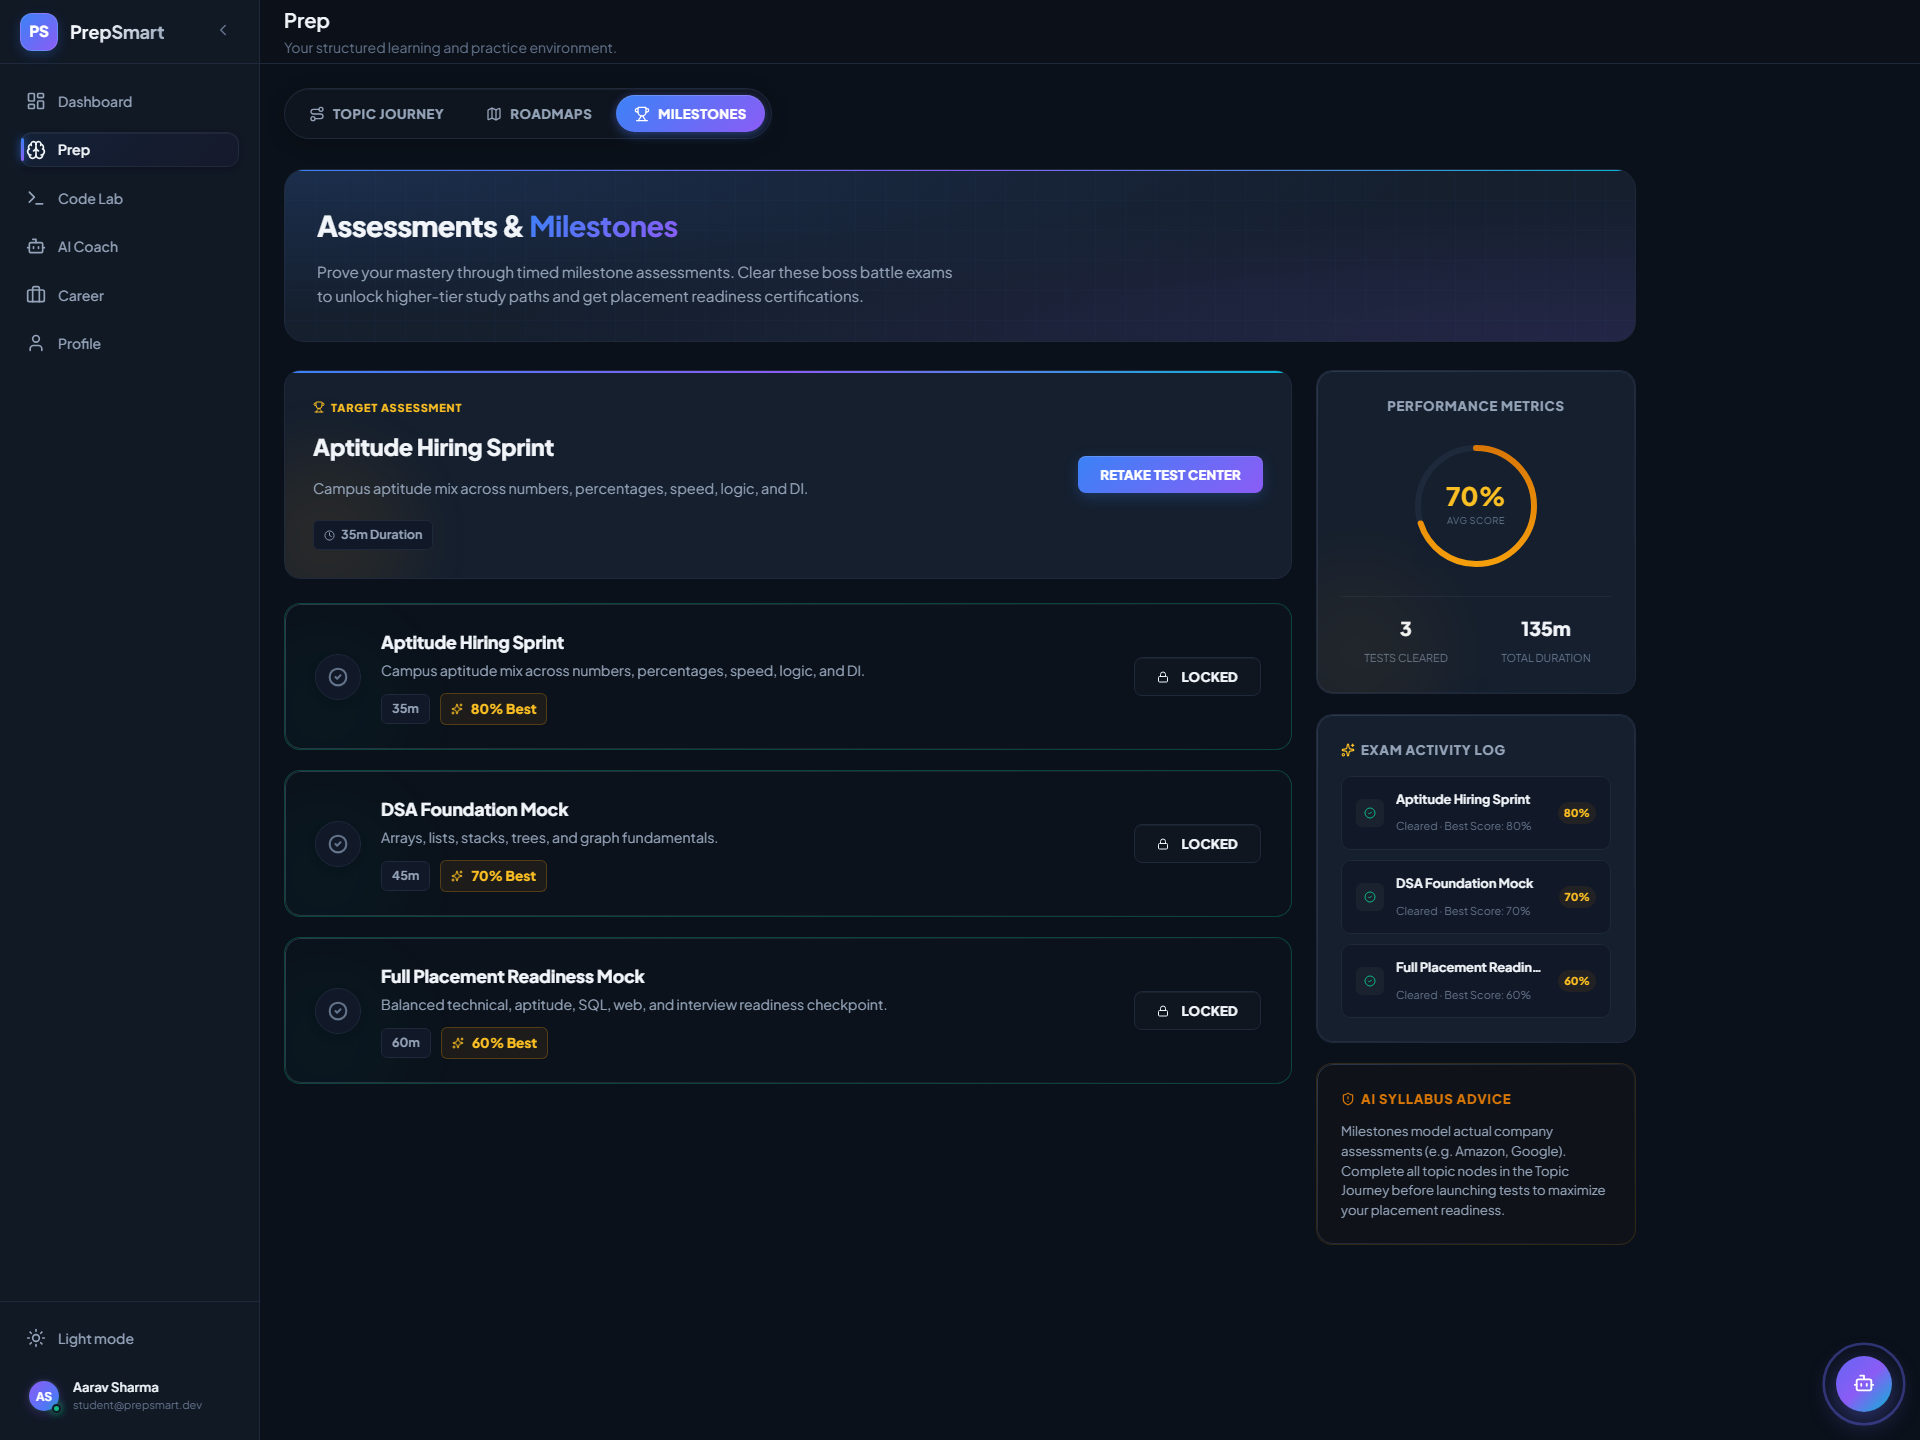
\includegraphics[width=0.95\textwidth]{Media/Chapter 5/milestones.png}
\caption{Learning Milestones}
\label{fig:milestones}
\end{figure}

Figure~\ref{fig:milestones} illustrates the milestone tracking interface. Each milestone represents an important stage within the placement preparation journey and consists of multiple learning activities or assessments.

Students attempt milestone assessments after completing the associated learning topics. The platform records milestone completion status, performance scores, and overall readiness before unlocking subsequent preparation stages.

This structured evaluation approach enables students to monitor their preparation systematically while ensuring that essential concepts are mastered before progressing further.

\subsubsection*{Major Features}

\begin{itemize}

\item Milestone-based assessments.

\item Preparation stage tracking.

\item Automatic progress updates.

\item Learning checkpoint evaluation.

\item Readiness verification.

\item Dashboard integration.

\end{itemize}

\subsection{Topic Study}

The Topic Study interface provides comprehensive learning material for individual subjects included within the placement preparation roadmap. It serves as the primary study environment where students learn theoretical concepts before attempting quizzes, coding exercises, and mock interviews.

\begin{figure}[H]
\centering
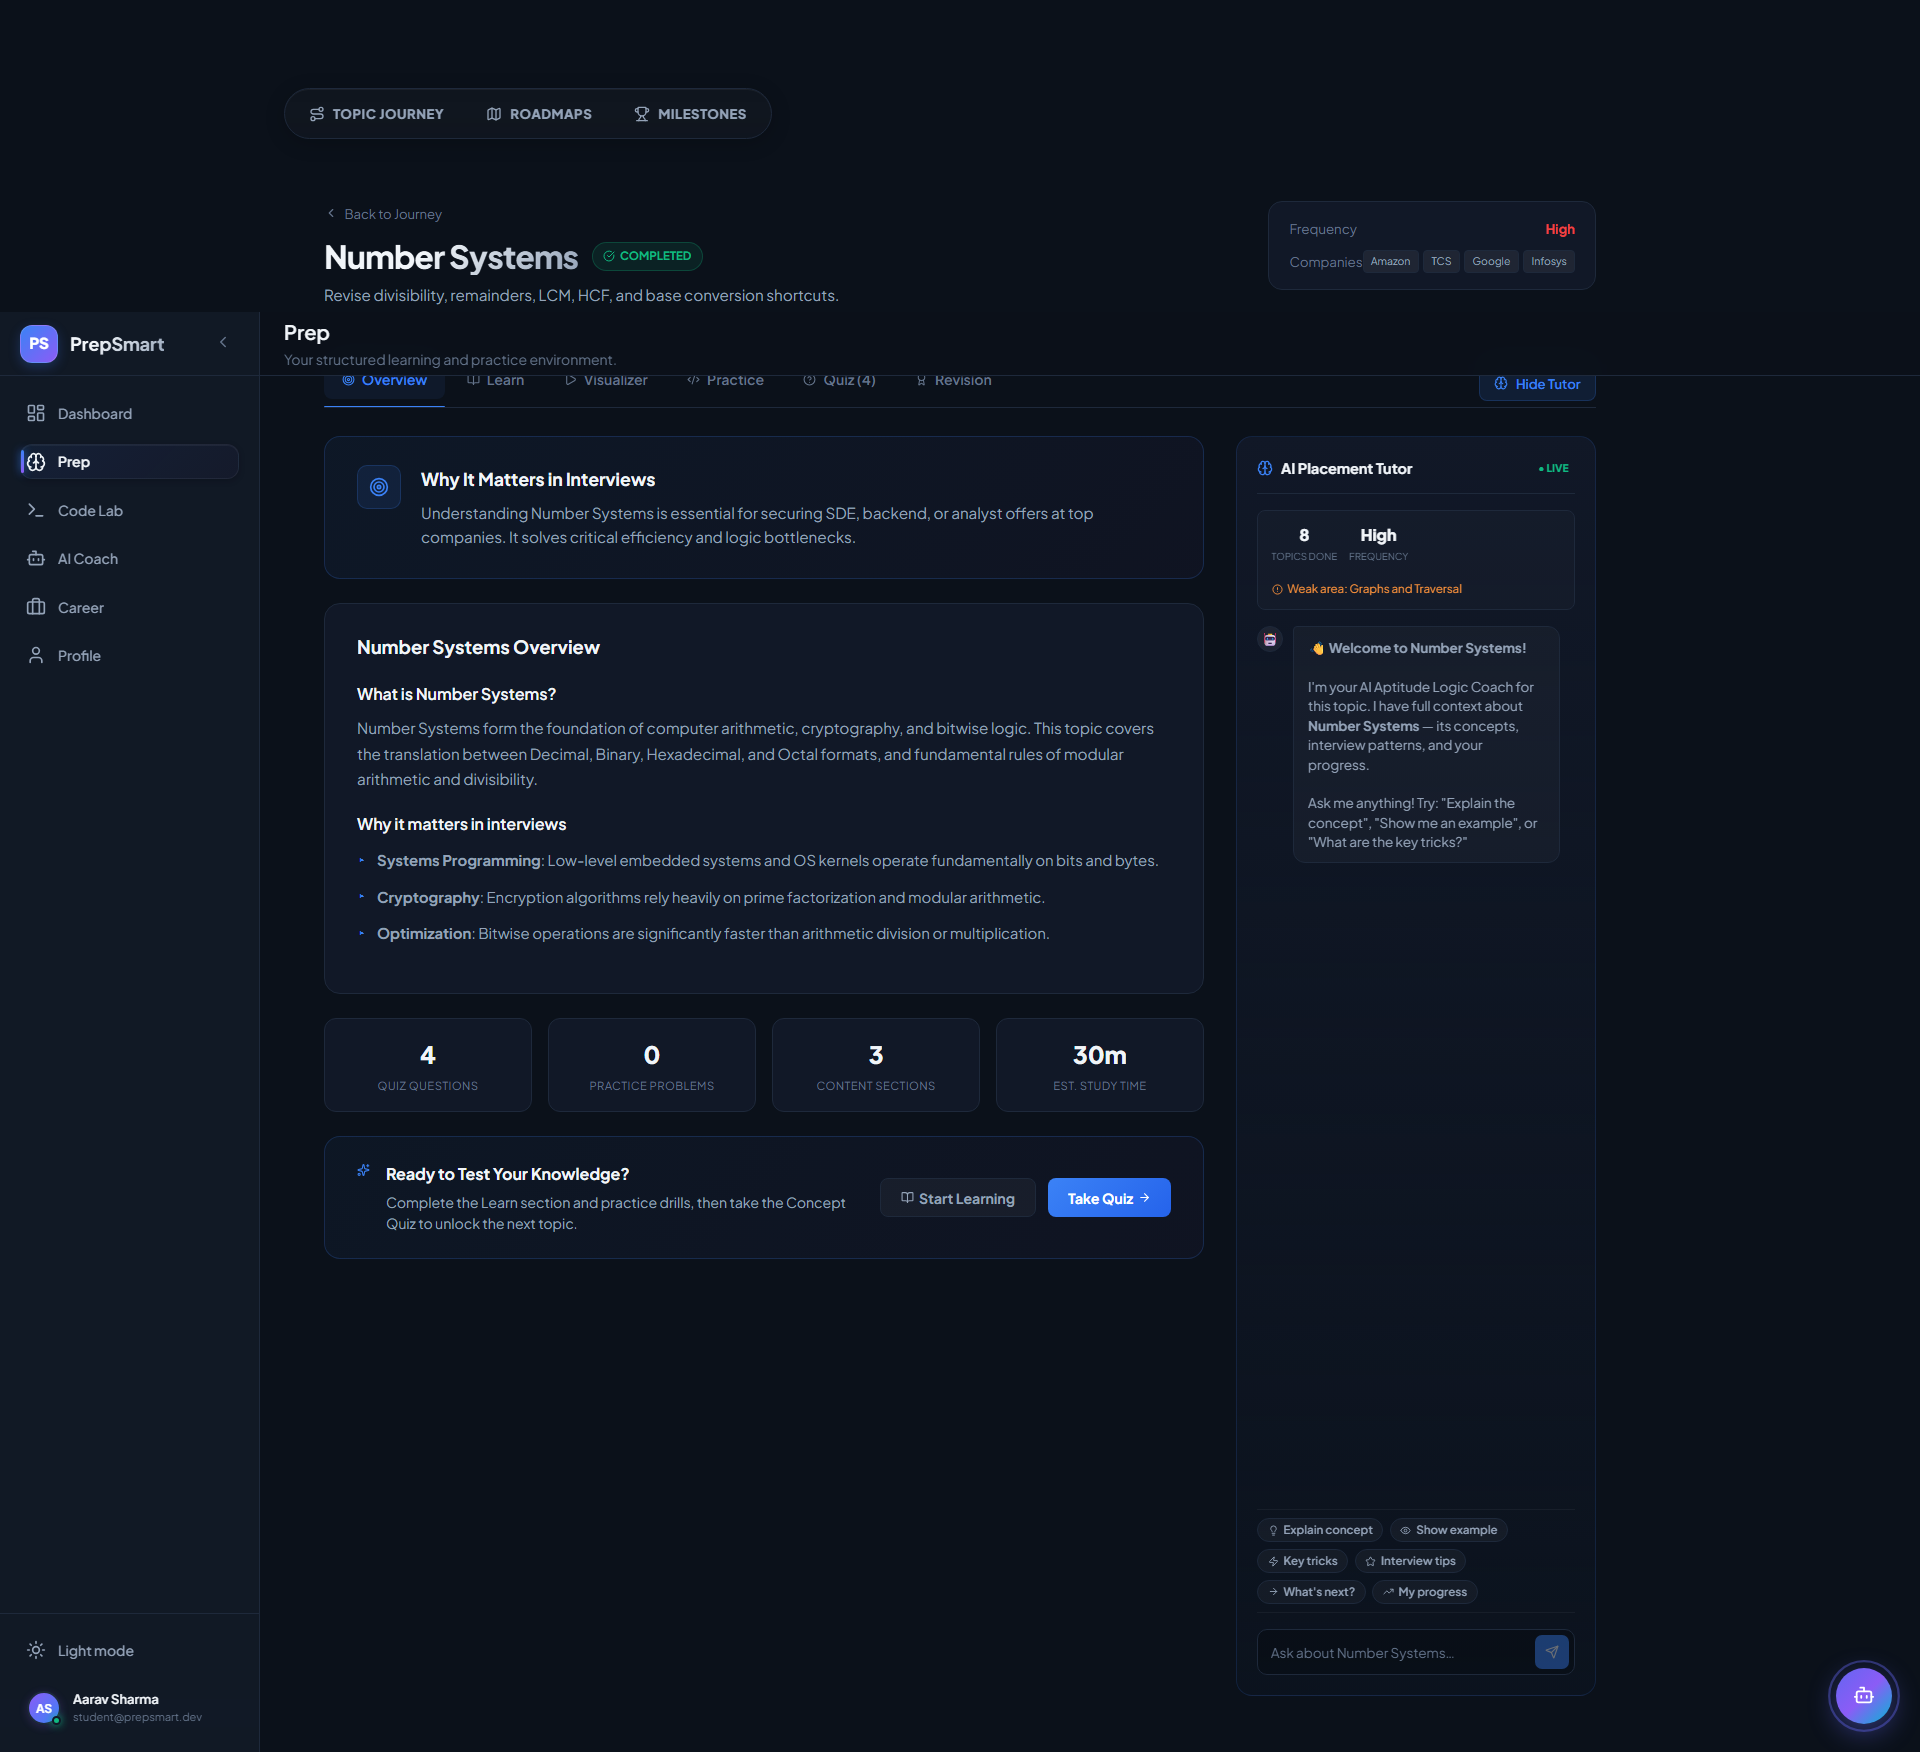
\includegraphics[width=0.95\textwidth]{Media/Chapter 5/topic_study.png}
\caption{Topic Study Interface}
\label{fig:topic_study}
\end{figure}

Figure~\ref{fig:topic_study} presents the Topic Study interface. This page displays detailed learning material, explanations, examples, and related resources for the selected topic.

Students can navigate through different sections of the learning material while monitoring their completion status. After finishing the theoretical content, users can proceed to quizzes, coding practice, or milestone assessments to evaluate their understanding.

The interface combines educational content with progress tracking, enabling students to complete each topic systematically while maintaining consistency throughout their placement preparation journey.

\subsubsection*{Major Features}

\begin{itemize}

\item Topic-wise learning material.

\item Structured educational content.

\item Progress tracking.

\item Easy topic navigation.

\item Integration with quizzes.

\item Direct continuation to coding practice and assessments.

\end{itemize}

\section{Coding Practice Module}

The Coding Practice Module enables students to strengthen their programming skills through an integrated development environment within the PrepSmart platform. Instead of switching between multiple coding websites, students can solve programming problems, execute programs, participate in coding contests, and monitor their coding performance using a unified interface.

The module consists of four major interfaces: Problem Arena, Coding Workspace, Standalone Code Workspace, and Contest Hub. These interfaces collectively provide an interview-oriented programming environment that closely resembles modern online coding assessment platforms.

\subsection{Problem Arena}

The Problem Arena serves as the central repository of programming problems available within PrepSmart. It allows students to browse coding questions of varying difficulty levels and practice problems according to their preparation requirements.

\begin{figure}[H]
\centering
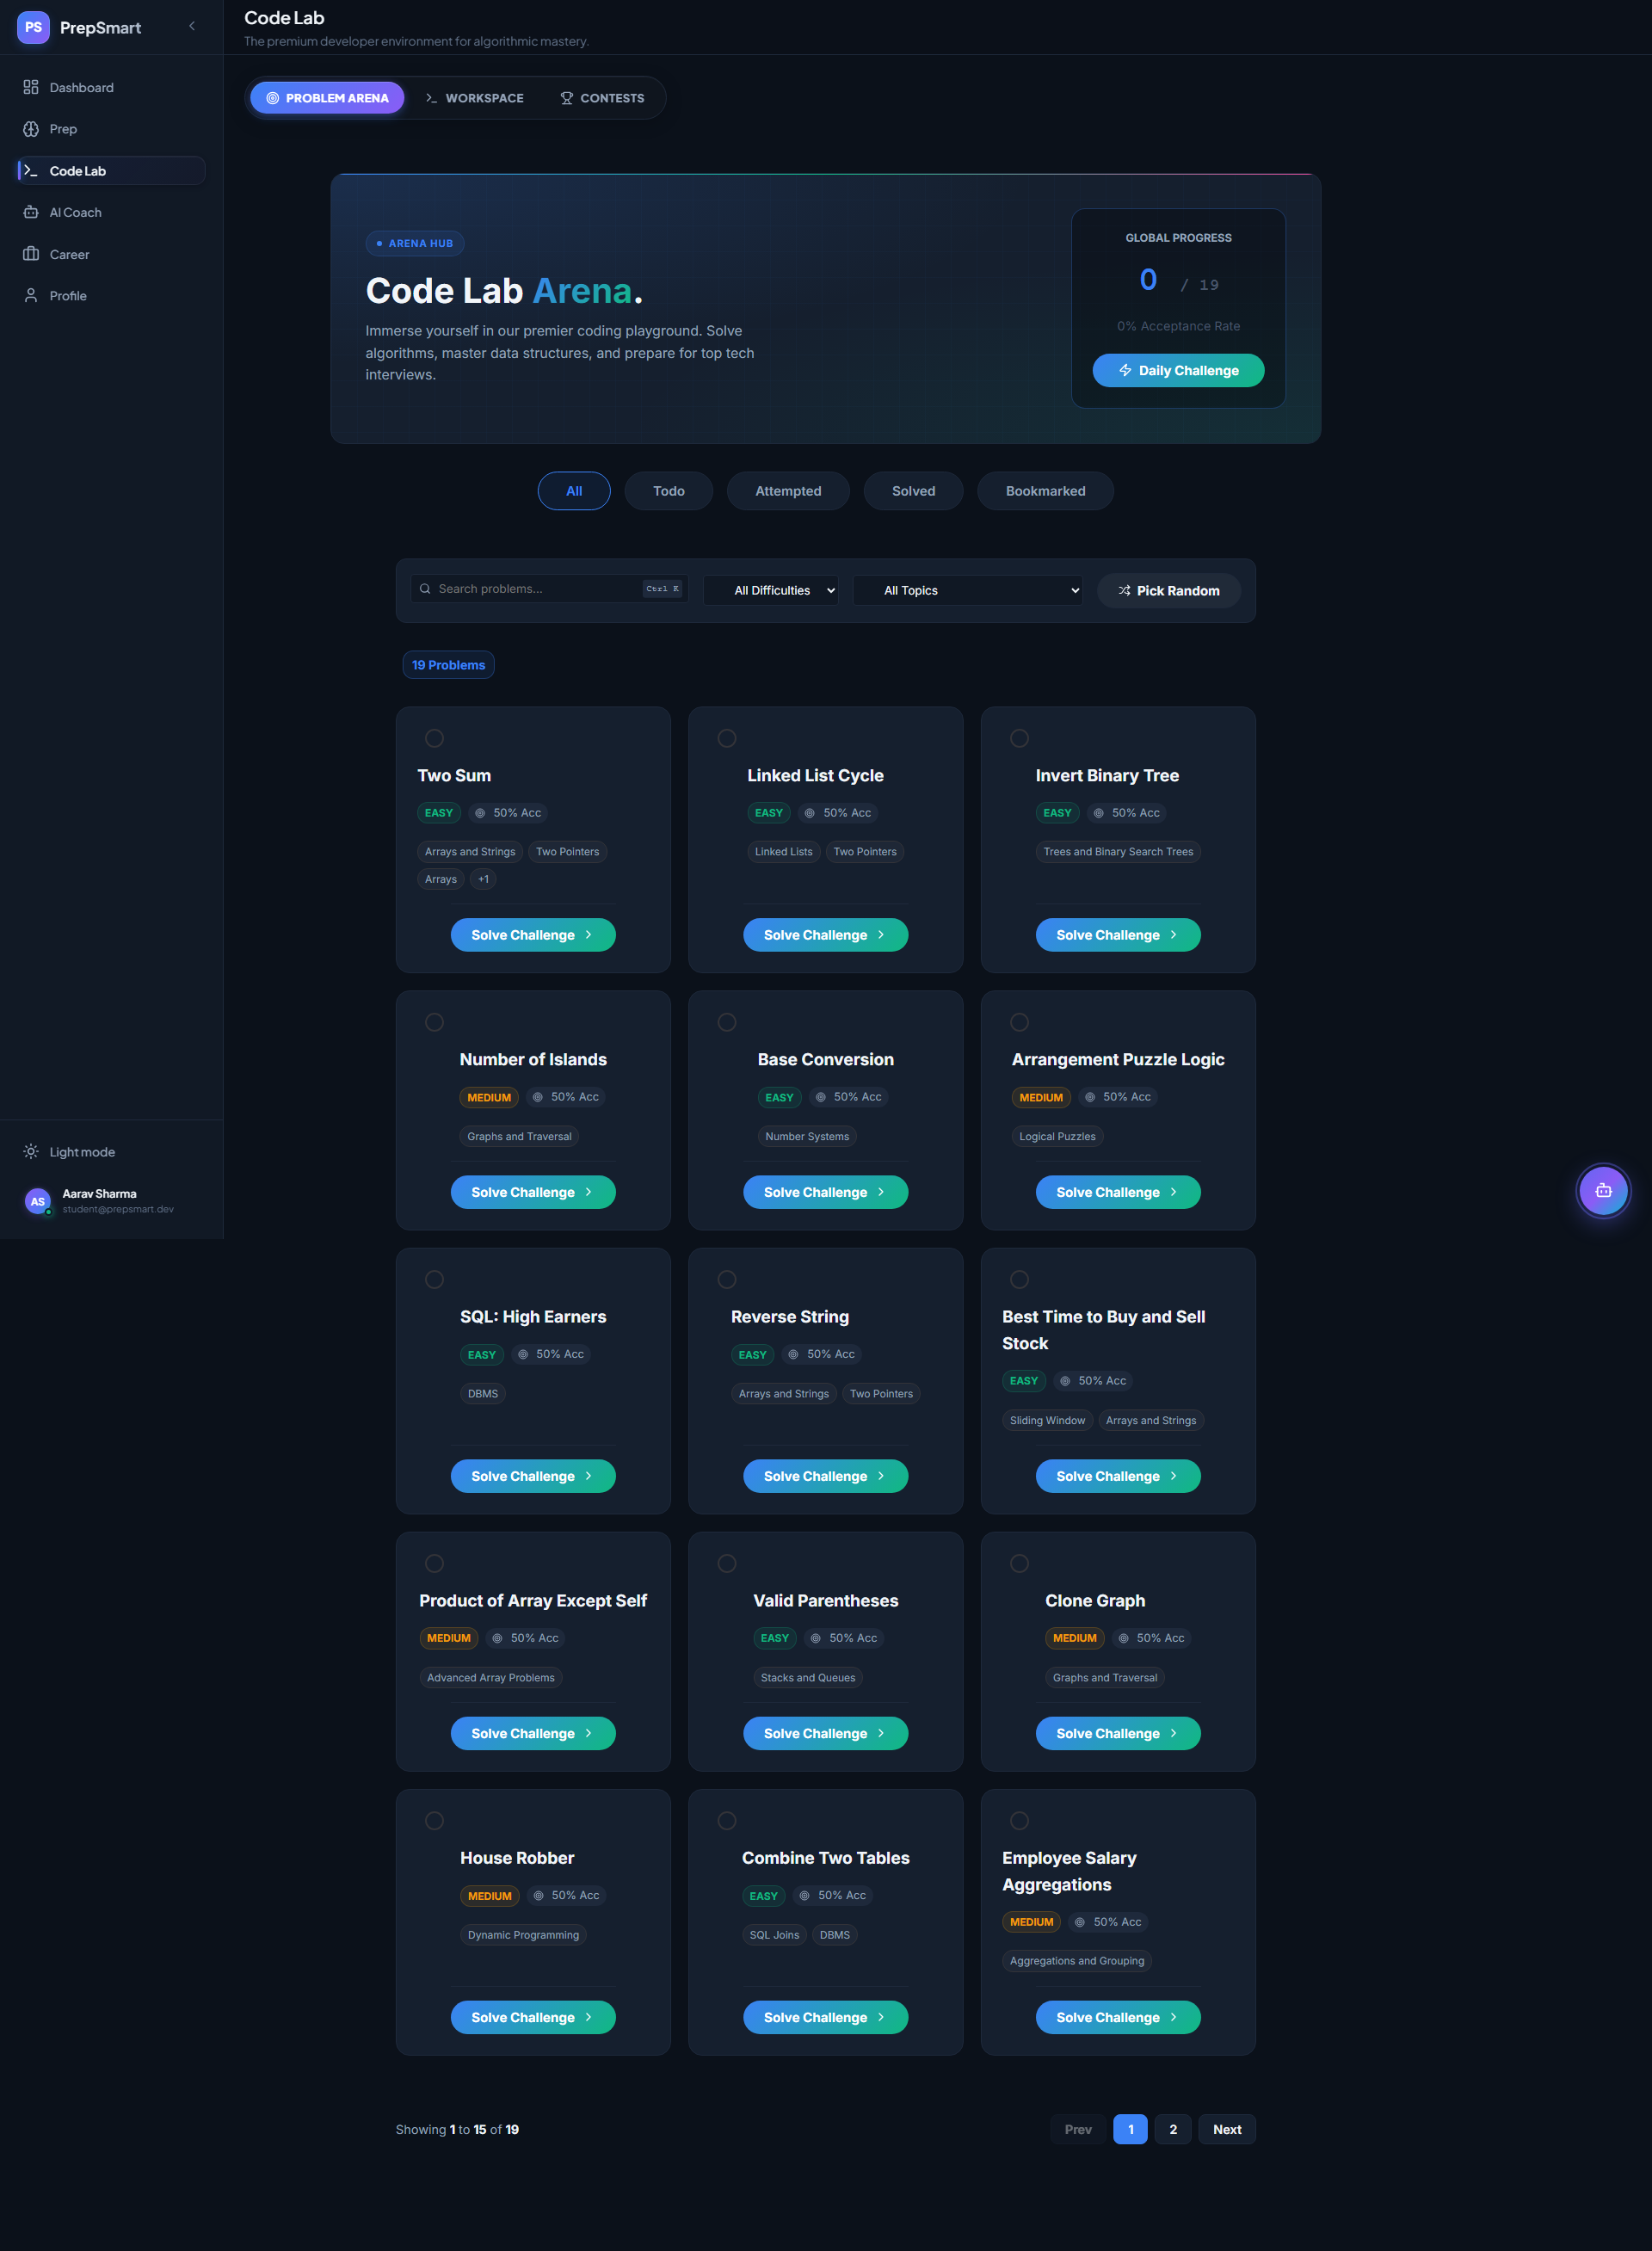
\includegraphics[width=0.95\textwidth]{Media/Chapter 5/problem_arena.png}
\caption{Problem Arena}
\label{fig:problem_arena}
\end{figure}

Figure~\ref{fig:problem_arena} illustrates the Problem Arena interface. This page displays the collection of programming problems available for practice. Students can browse problems based on difficulty level, topic, or interview relevance.

Each programming problem includes a title, difficulty level, associated topics, company tags, and other important information required before attempting the solution. The organized presentation allows students to efficiently select suitable problems according to their current preparation level.

The Problem Arena acts as the entry point to the coding environment and provides easy navigation to the coding workspace for solving selected problems.

\subsubsection*{Major Features}

\begin{itemize}

\item Collection of programming problems.

\item Difficulty-based problem categorization.

\item Topic-wise organization.

\item Company-specific problem tags.

\item Easy problem search and navigation.

\item Direct access to the coding workspace.

\end{itemize}

\subsection{Coding Workspace}

The Coding Workspace provides an integrated programming environment where students can write, execute, debug, and submit programming solutions. It closely simulates the coding environments commonly used during online placement assessments.

\begin{figure}[H]
\centering
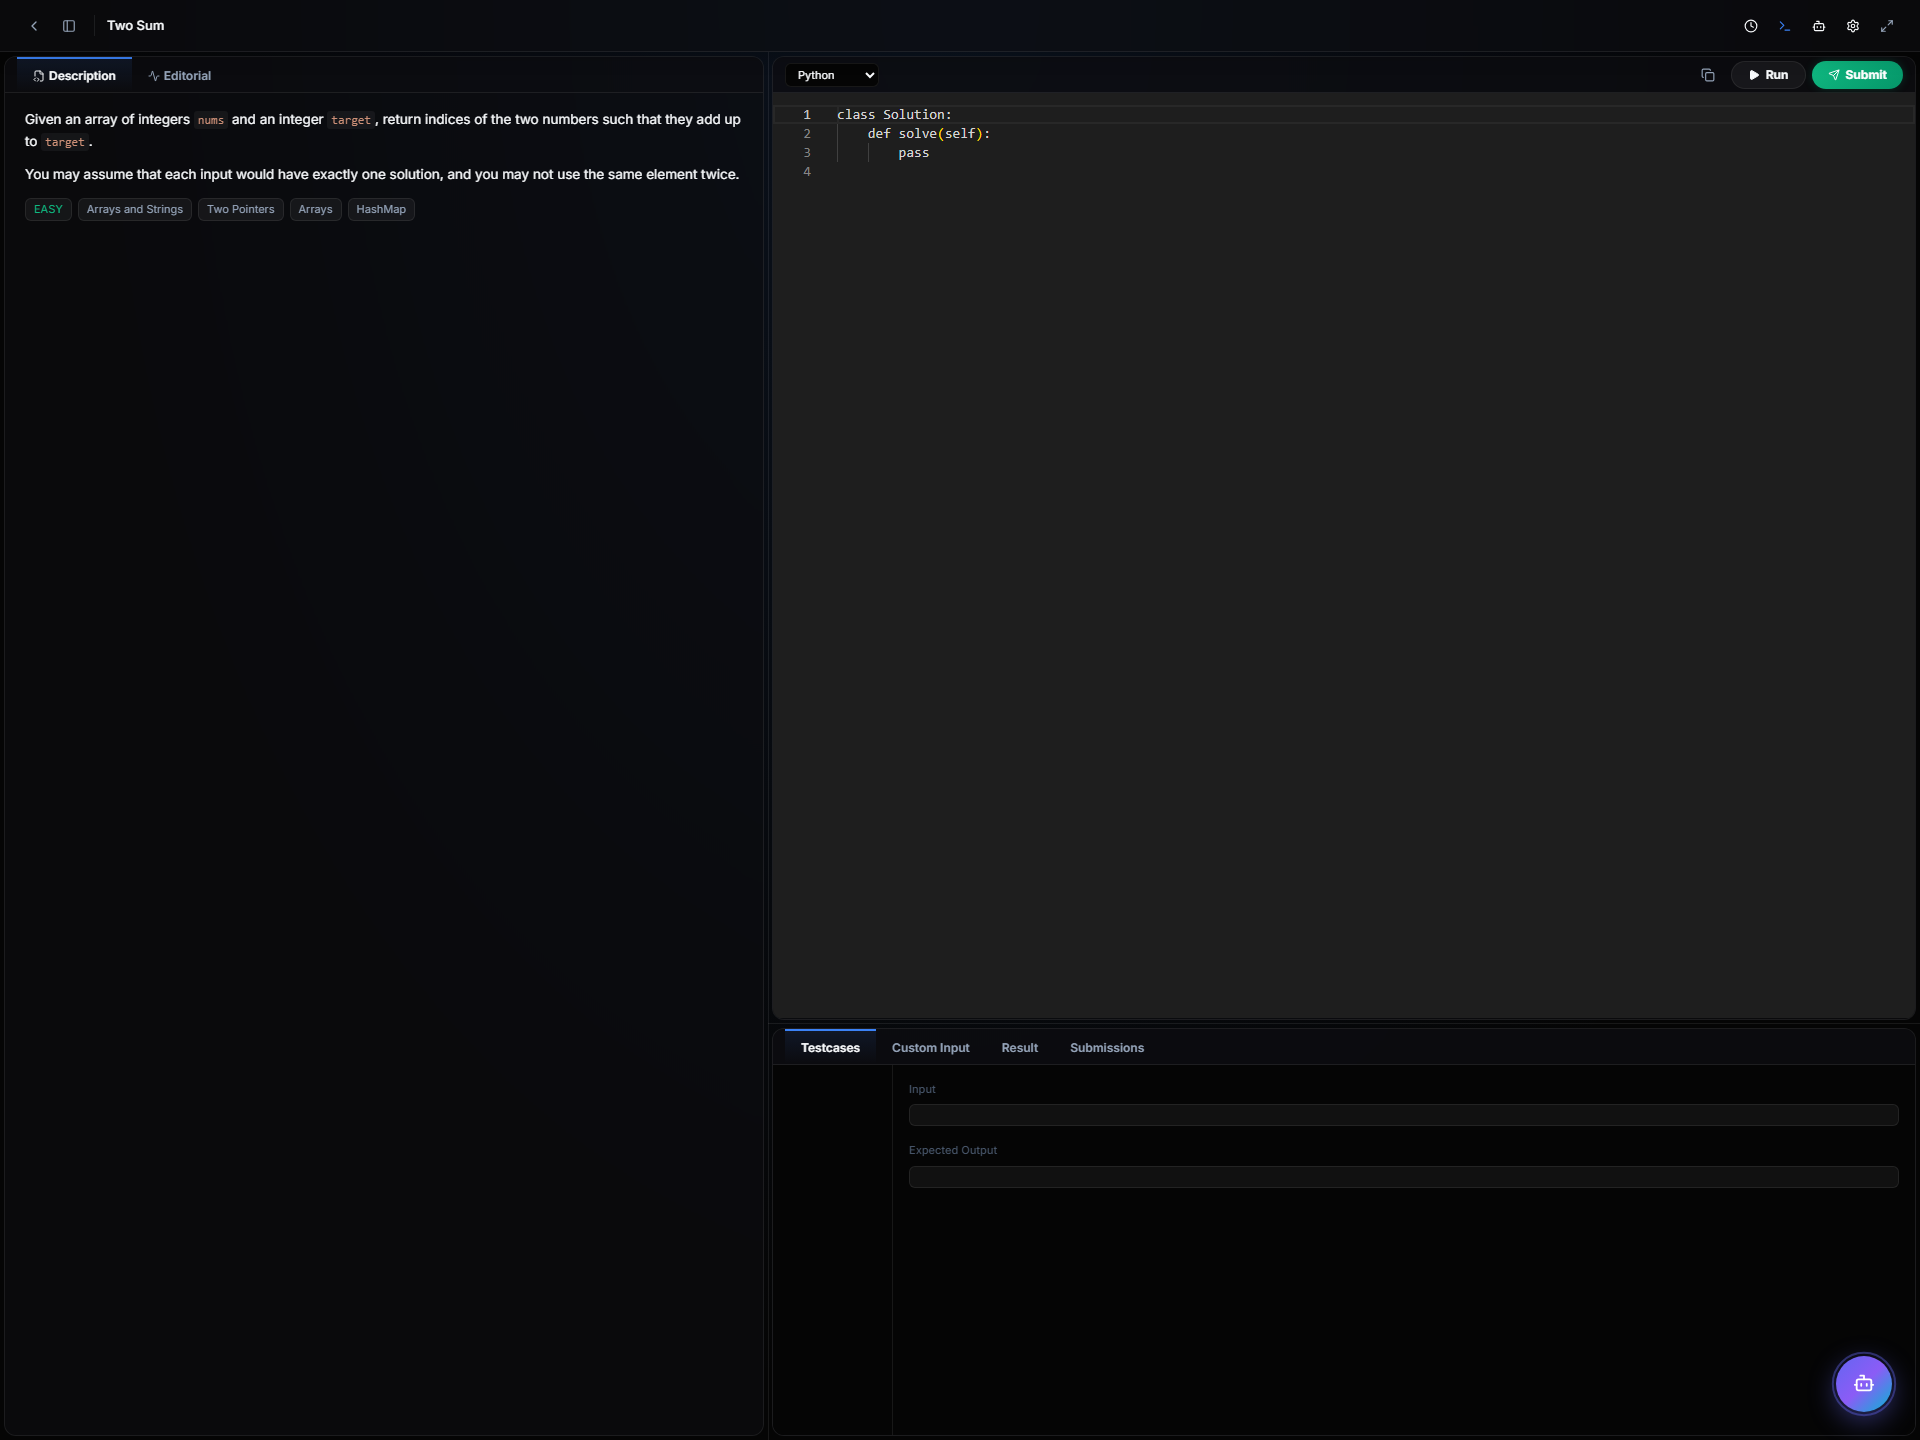
\includegraphics[width=0.95\textwidth]{Media/Chapter 5/coding_workspace.png}
\caption{Coding Workspace}
\label{fig:coding_workspace}
\end{figure}

Figure~\ref{fig:coding_workspace} presents the Coding Workspace of PrepSmart. The interface combines the problem statement, source code editor, programming language selection, custom input, execution controls, and output console within a single screen.

Students can write solutions using the integrated editor, execute programs with custom inputs, and verify the generated output before final submission. The platform also reports execution statistics such as runtime, execution status, and error messages, enabling students to debug their programs efficiently.

The integrated design minimizes distractions by providing all programming resources within a unified coding environment.

\subsubsection*{Major Features}

\begin{itemize}

\item Integrated source code editor.

\item Programming language selection.

\item Custom input execution.

\item Output console.

\item Runtime and error reporting.

\item Program submission facility.

\end{itemize}

\subsection{Standalone Code Workspace}

The Standalone Code Workspace enables students to write and execute programs independently without selecting a predefined coding problem. This interface is useful for experimenting with programming concepts, debugging code, and practicing algorithms freely.

\begin{figure}[H]
\centering
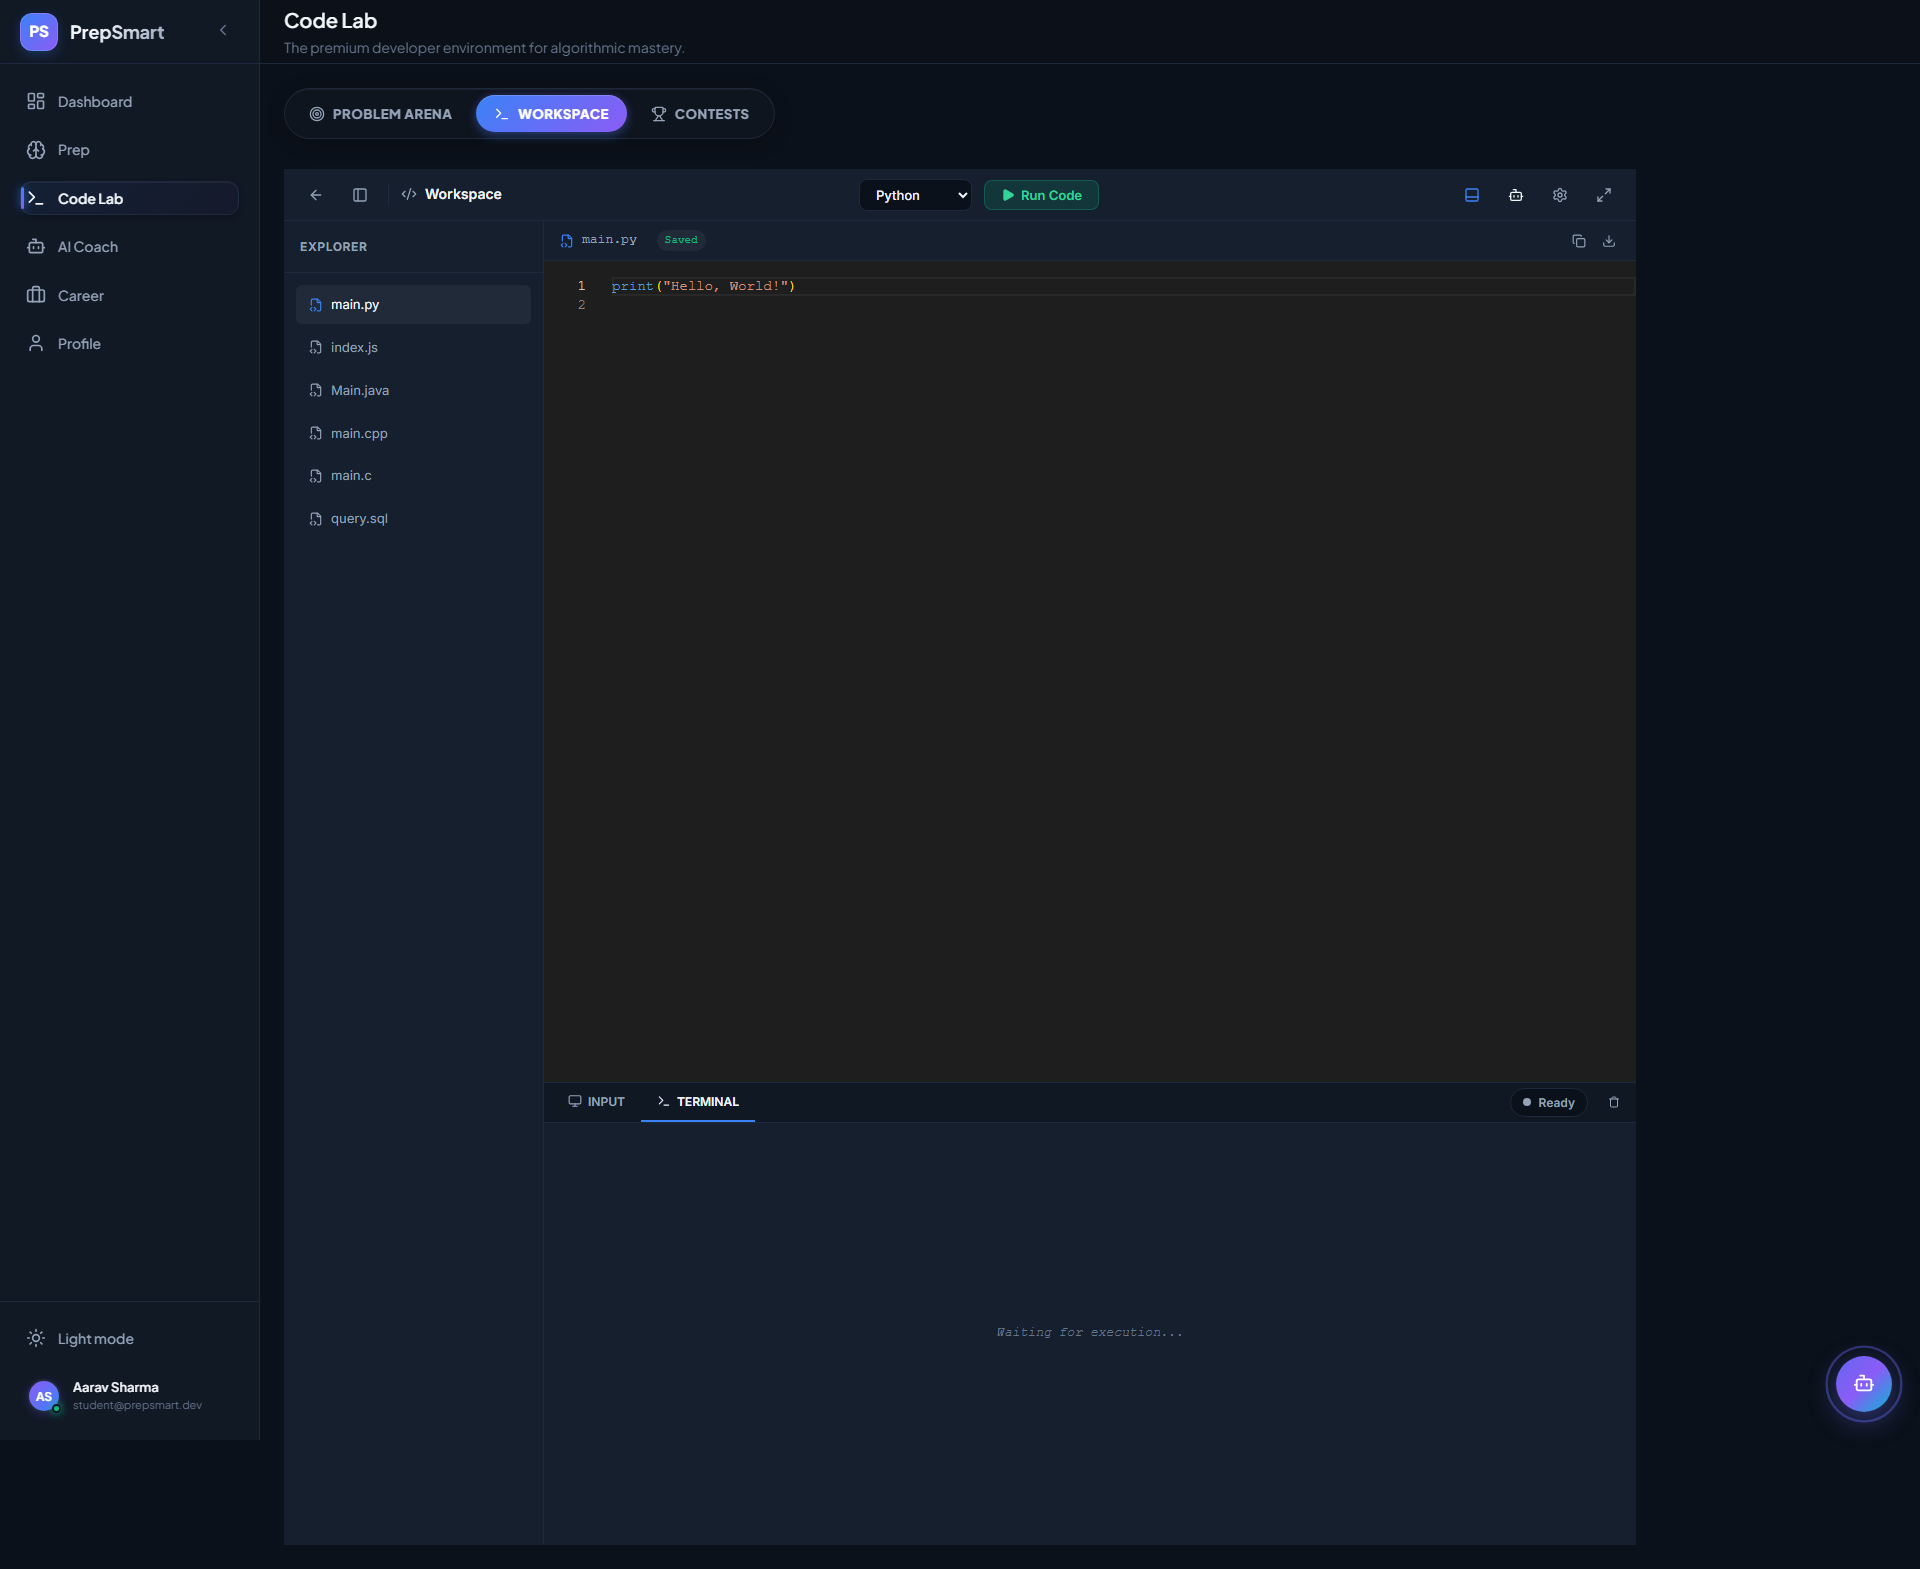
\includegraphics[width=0.95\textwidth]{Media/Chapter 5/standalone_workspace.png}
\caption{Standalone Code Workspace}
\label{fig:standalone_workspace}
\end{figure}

Figure~\ref{fig:standalone_workspace} illustrates the Standalone Code Workspace. Unlike the problem-specific coding environment, this workspace allows students to develop and execute programs without predefined constraints or evaluation criteria.

The interface provides a programming editor, language selection, execution controls, and an output console. Students can use this environment for experimenting with programming techniques, verifying algorithm implementations, or practicing coding concepts before attempting formal programming challenges.

\subsubsection*{Major Features}

\begin{itemize}

\item Independent programming environment.

\item Custom code execution.

\item Multi-language support.

\item Output visualization.

\item Algorithm experimentation.

\item Debugging assistance.

\end{itemize}

\subsection{Contest Hub}

The Contest Hub provides students with information about ongoing and upcoming programming contests from multiple competitive coding platforms. It encourages students to participate in real-world programming competitions and improve their problem-solving abilities.

\begin{figure}[H]
\centering
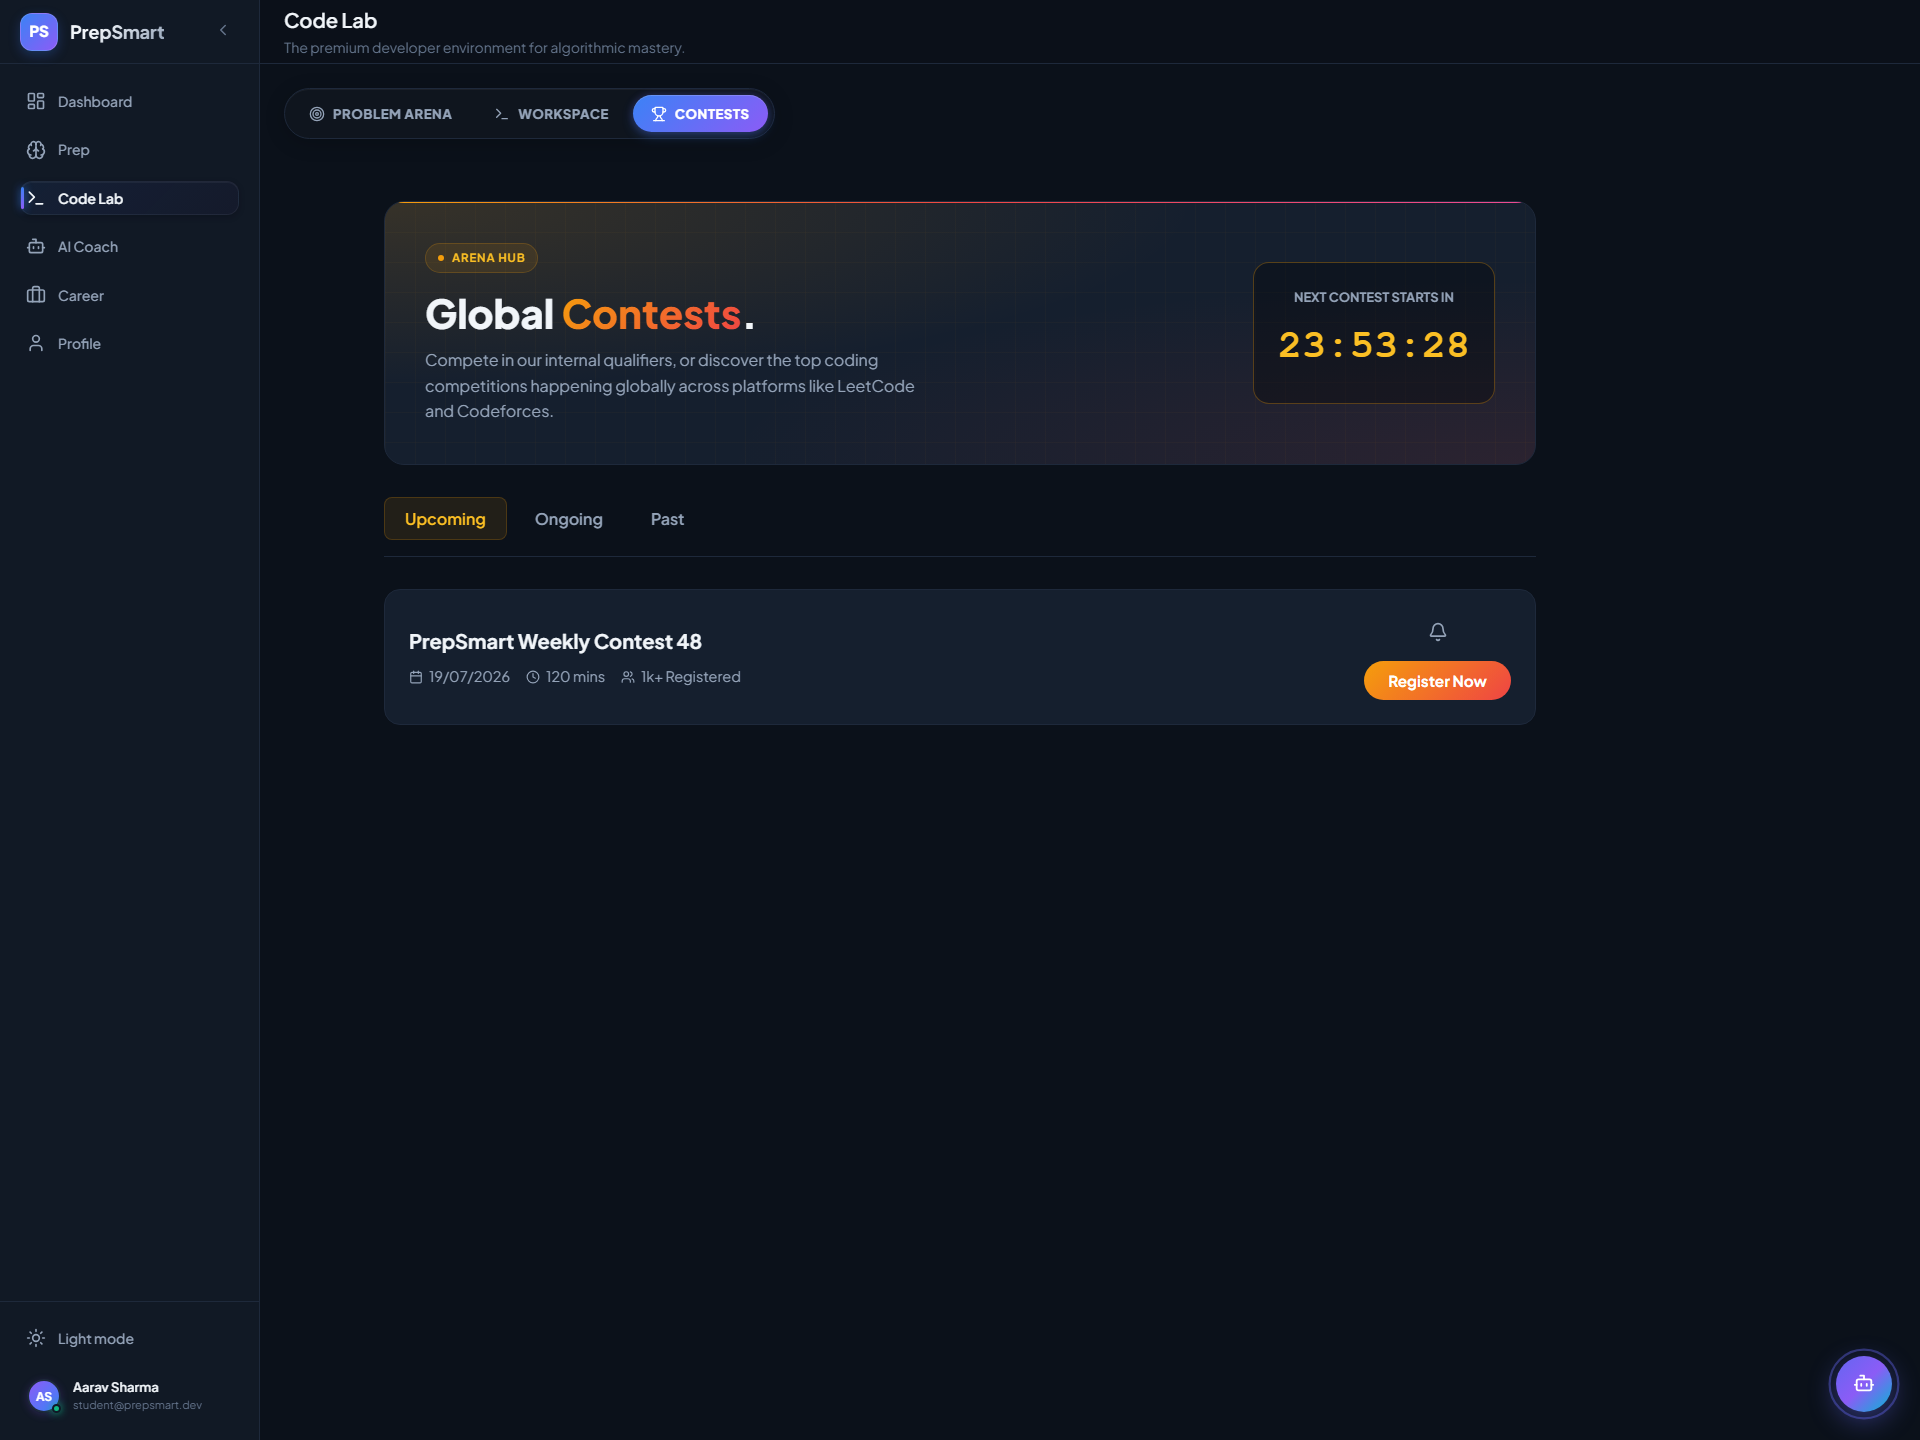
\includegraphics[width=0.95\textwidth]{Media/Chapter 5/contest_hub.png}
\caption{Contest Hub}
\label{fig:contest_hub}
\end{figure}

Figure~\ref{fig:contest_hub} presents the Contest Hub interface of PrepSmart. The page displays programming contests collected from external coding platforms and presents information such as contest names, start times, durations, hosting platforms, and registration links.

Students can easily browse upcoming contests and participate directly from the platform. The centralized presentation of contest information eliminates the need to visit multiple coding websites individually and encourages continuous participation in competitive programming activities.

\subsubsection*{Major Features}

\begin{itemize}

\item Display of upcoming coding contests.

\item Contest platform information.

\item Contest schedules.

\item Registration links.

\item Integration with external contest providers.

\item Encouragement for competitive programming.

\end{itemize}

\section{AI Interview Module}

The AI Interview Module provides students with an interactive interview preparation environment that simulates technical interviews using Artificial Intelligence. Unlike conventional interview preparation methods, this module enables students to answer technical questions, receive automated feedback, and evaluate their interview readiness within the PrepSmart platform.

The interface is designed to improve communication skills, technical understanding, and confidence by providing a realistic interview experience. Students can practice repeatedly while monitoring their improvement over time.

\begin{figure}[H]
\centering
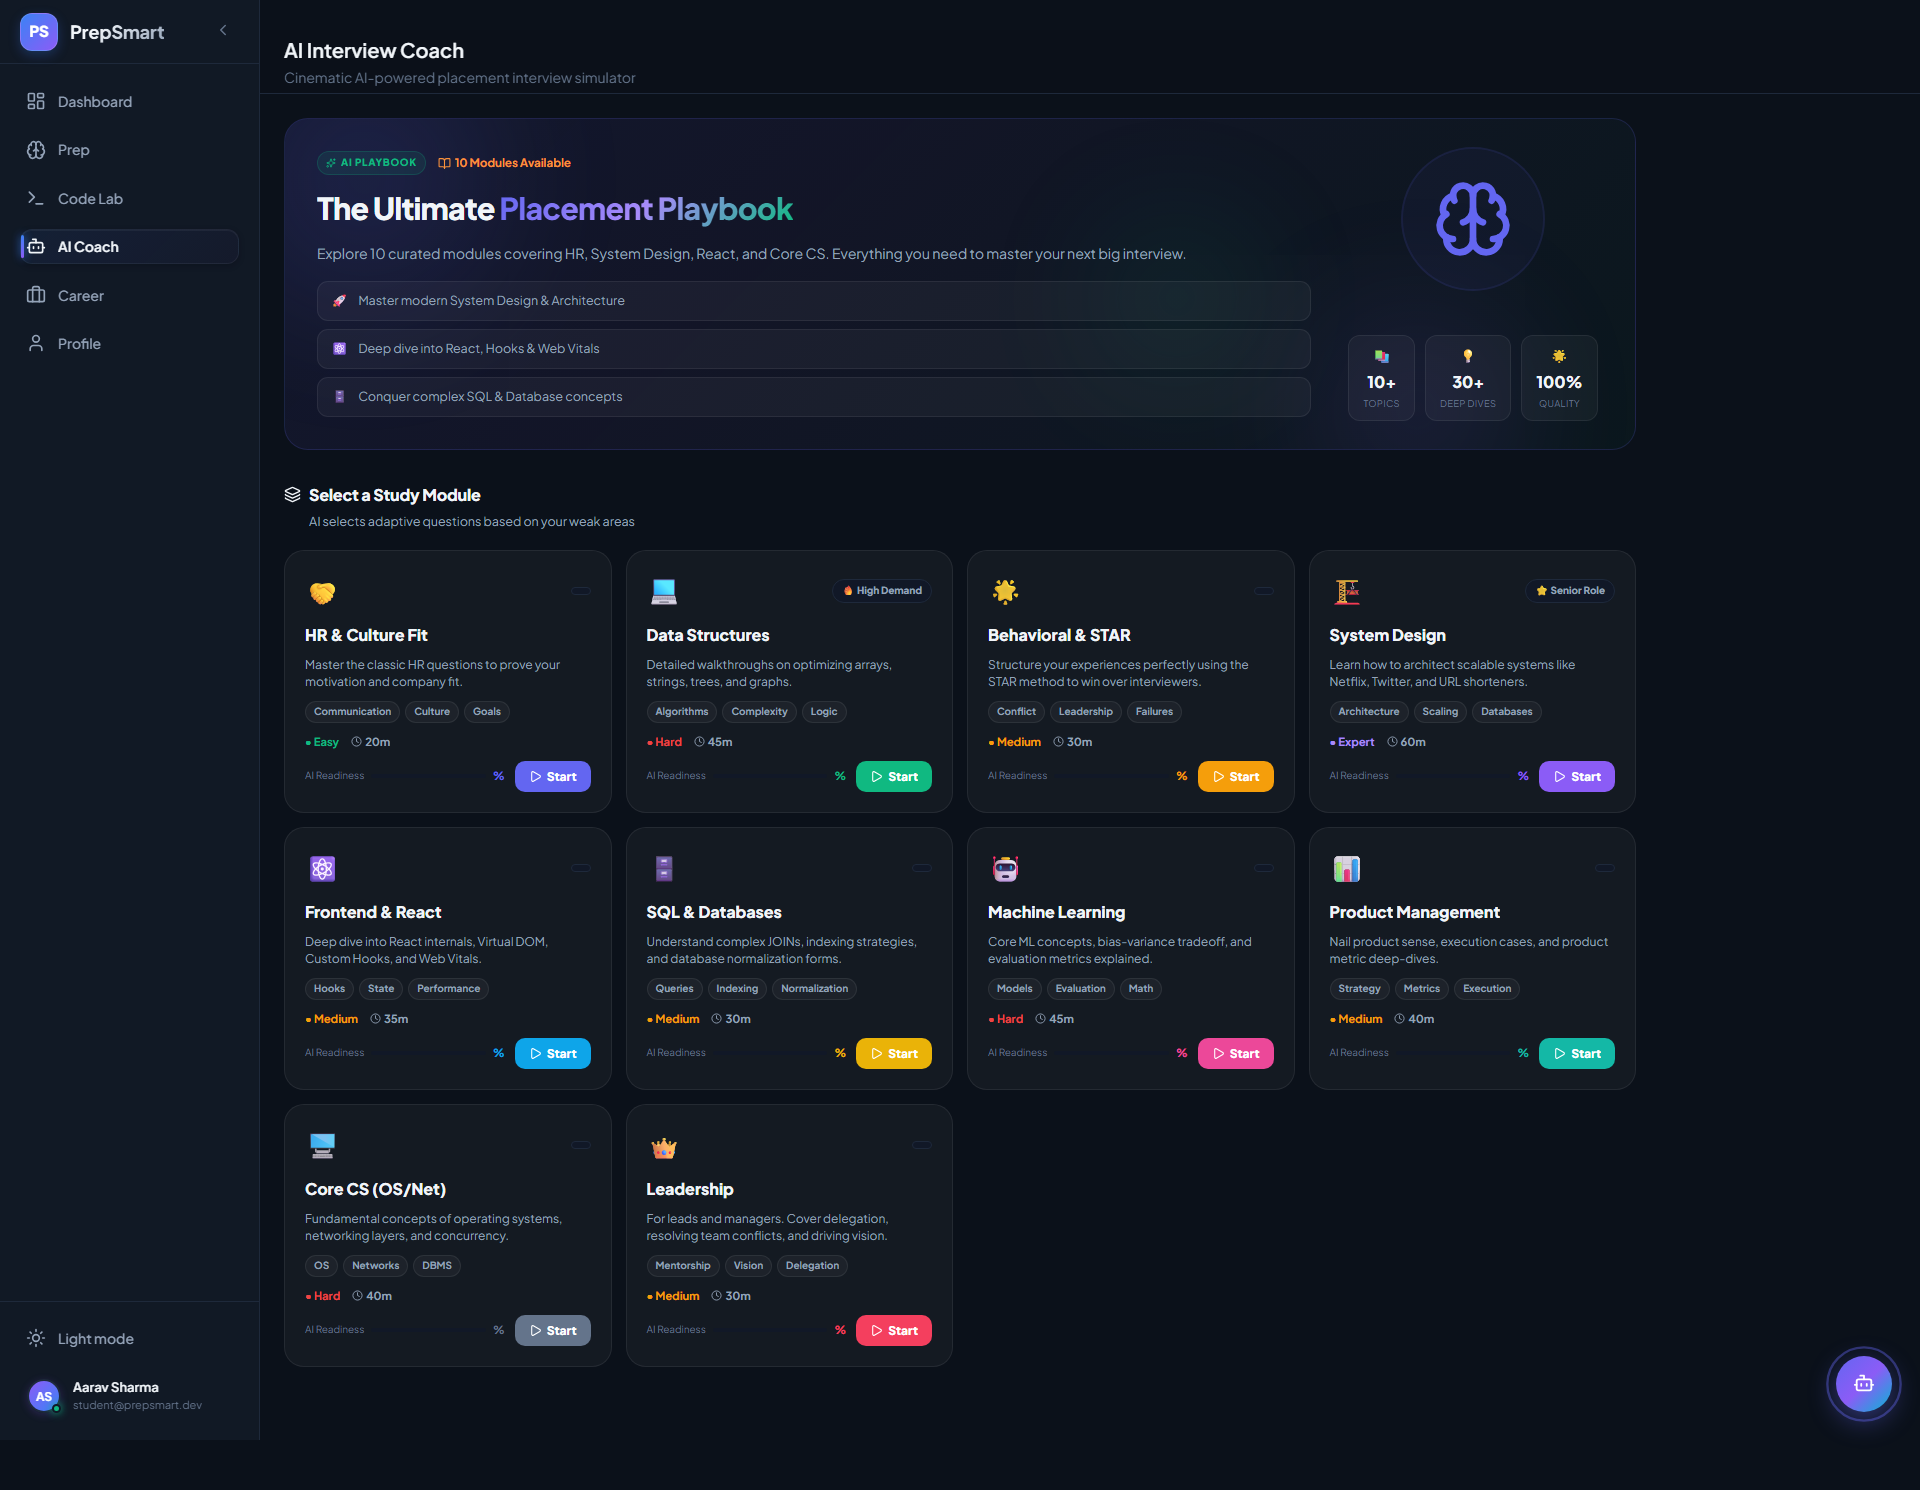
\includegraphics[width=0.95\textwidth]{Media/Chapter 5/ai_interview.png}
\caption{AI Interview Interface}
\label{fig:ai_interview}
\end{figure}

Figure~\ref{fig:ai_interview} illustrates the AI Interview interface of PrepSmart. The page allows students to participate in simulated interview sessions by selecting interview categories and answering technical questions presented by the system.

During an interview session, each response submitted by the student is evaluated by the backend, and AI-generated feedback is provided to highlight strengths, weaknesses, and possible improvements. The interface also maintains interview progress and displays evaluation results in an organized manner.

By providing immediate feedback and realistic interview practice, the module enables students to strengthen both technical knowledge and communication skills before attending actual placement interviews.

\subsection*{Major Features}

\begin{itemize}

\item AI-assisted interview simulation.

\item Technical question evaluation.

\item Automated feedback generation.

\item Interview progress tracking.

\item Performance scoring.

\item Interview history management.

\end{itemize}

\section{Company Preparation Module}

The Company Preparation Module enables students to prepare specifically for companies participating in campus recruitment. Instead of following a general preparation strategy, students can explore company-specific requirements, monitor their readiness, and identify the topics that require further improvement.

The module provides separate interfaces for viewing available companies and detailed preparation information for each selected company.

\subsection{Companies}

The Companies interface displays the list of organizations available within the PrepSmart platform. Students can browse companies and select the organization for which they wish to evaluate their preparation.

\begin{figure}[H]
\centering
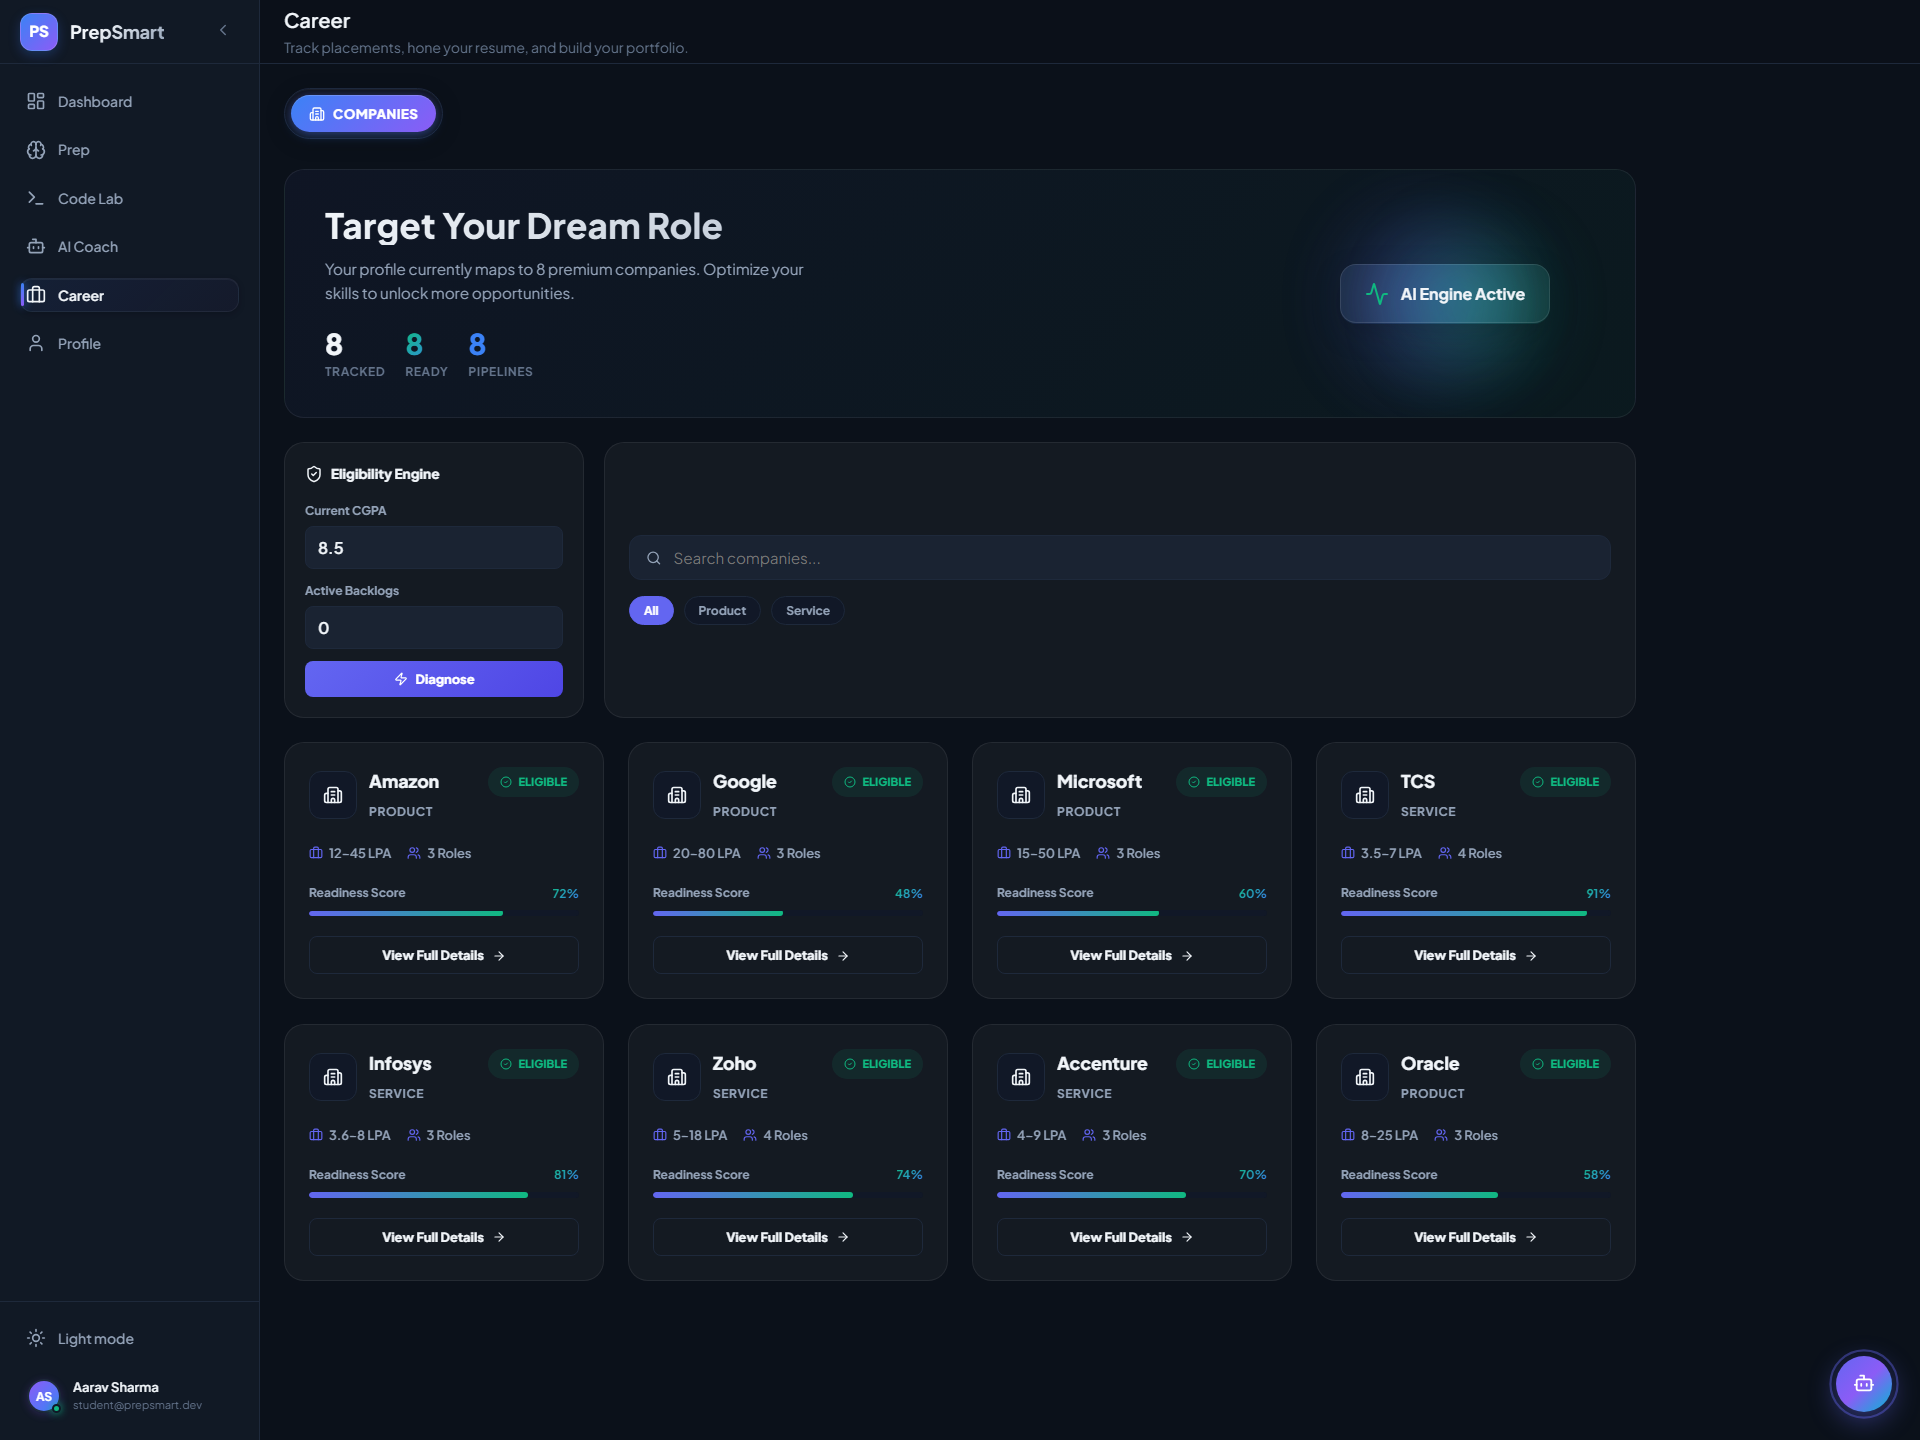
\includegraphics[width=0.95\textwidth]{Media/Chapter 5/companies.png}
\caption{Companies Interface}
\label{fig:companies}
\end{figure}

Figure~\ref{fig:companies} presents the Companies interface of PrepSmart. The page provides an organized list of target companies together with essential preparation information. Students can browse available organizations and select a company to view detailed preparation requirements.

The interface acts as the starting point for company-specific preparation and provides quick navigation to detailed readiness information.

\subsubsection*{Major Features}

\begin{itemize}

\item List of target companies.

\item Company search.

\item Company selection.

\item Quick navigation.

\item Preparation overview.

\end{itemize}

\subsection{Company Details}

The Company Details interface provides comprehensive information regarding the selected company's preparation requirements and the student's readiness status.

\begin{figure}[H]
\centering
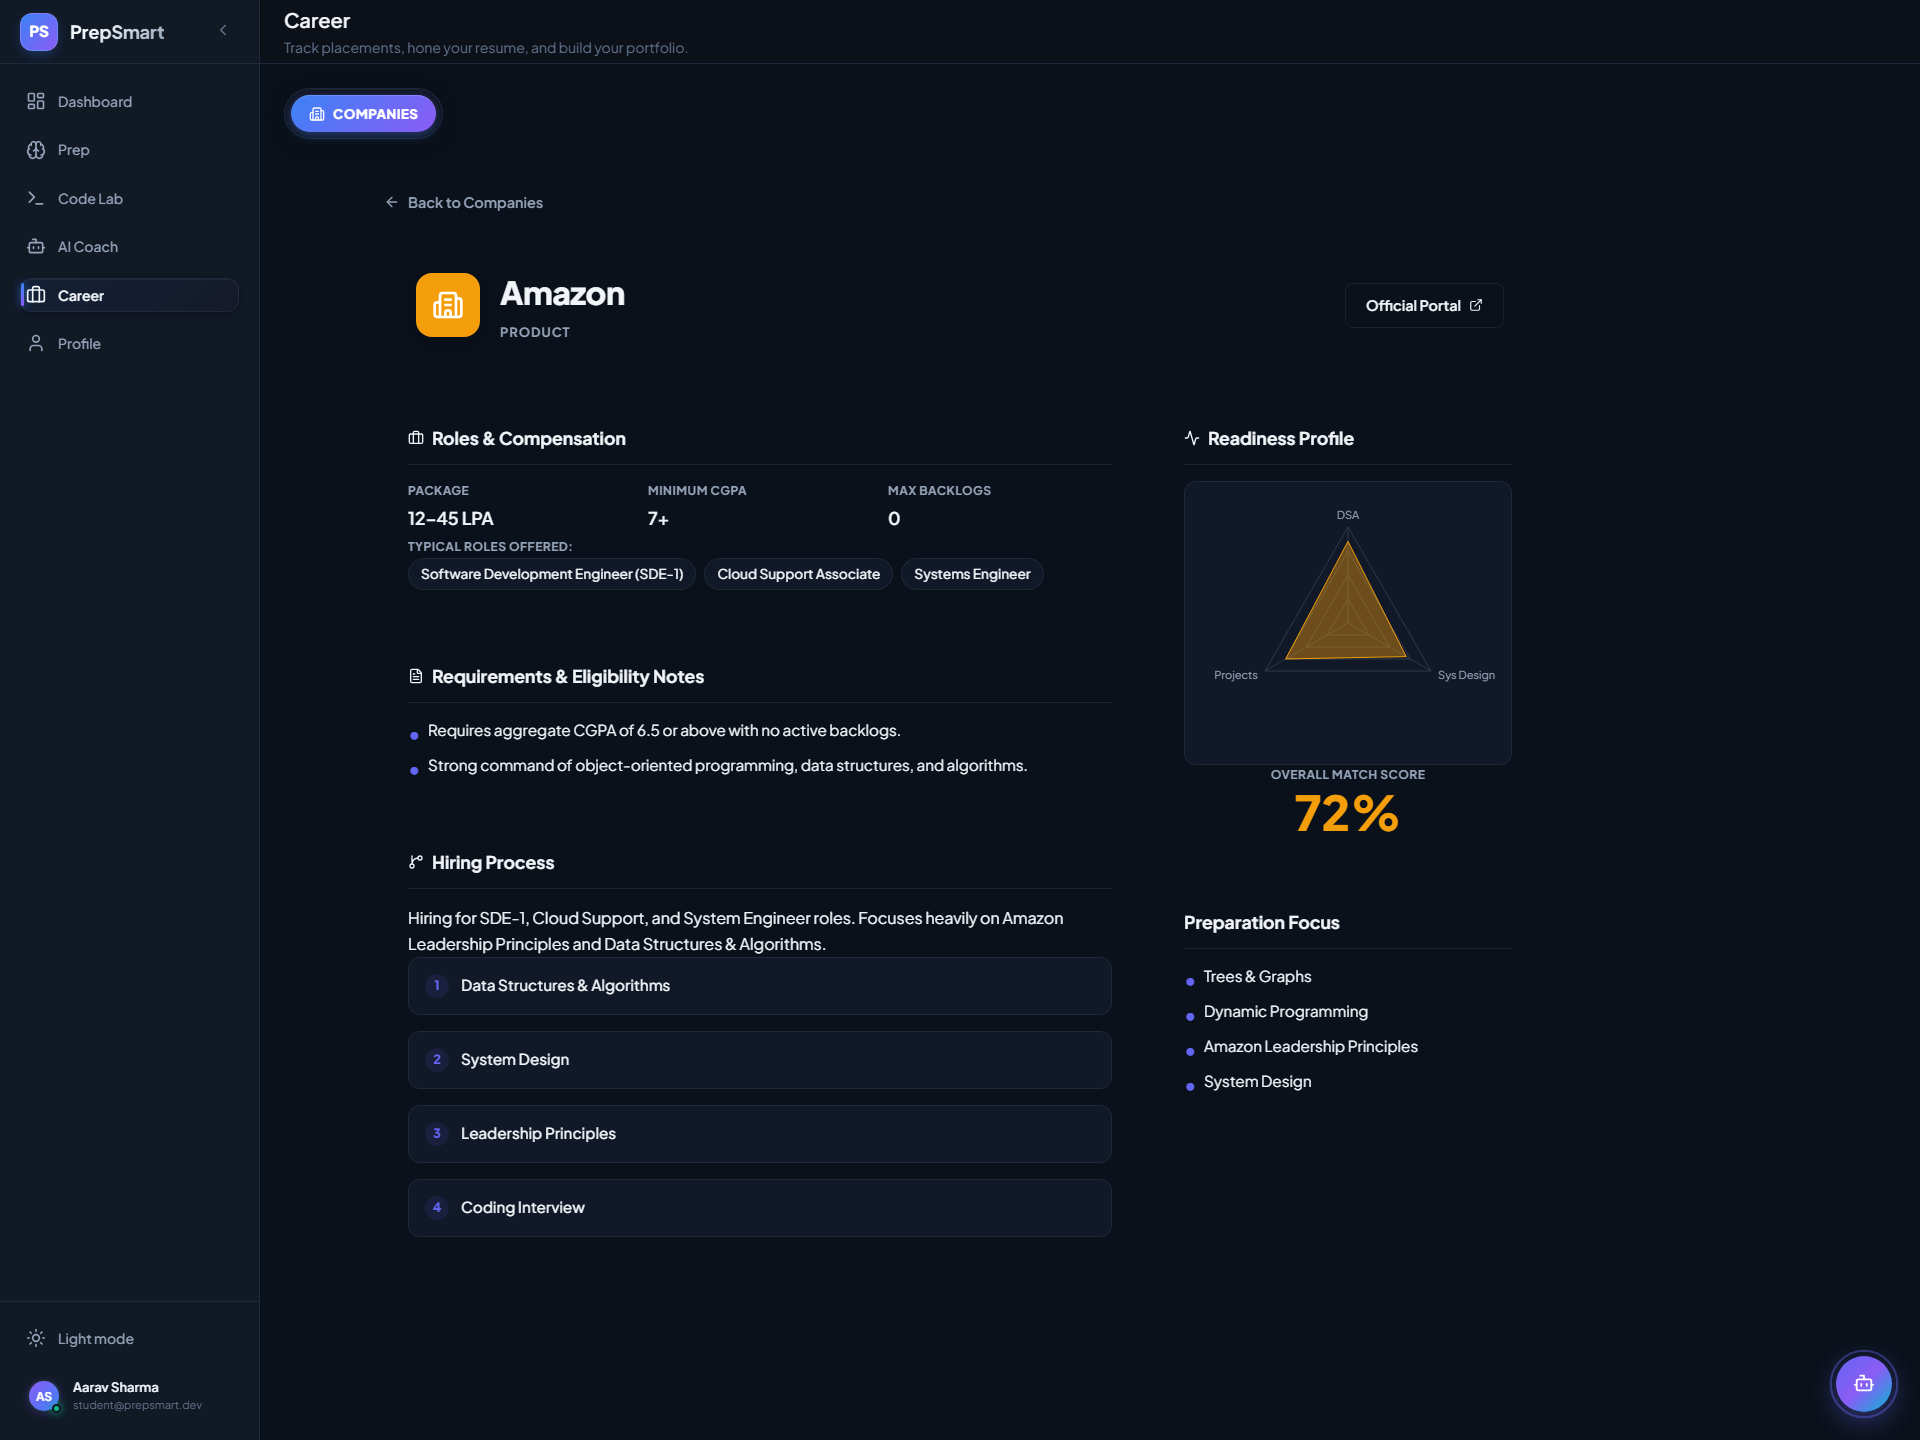
\includegraphics[width=0.95\textwidth]{Media/Chapter 5/company_detail.png}
\caption{Company Details Interface}
\label{fig:company_detail}
\end{figure}

Figure~\ref{fig:company_detail} illustrates the Company Details interface. This page presents company-specific preparation information including recommended topics, readiness indicators, coding expectations, interview requirements, and preparation progress.

The platform analyzes the student's completed learning activities and compares them with the selected company's expected preparation profile. Based on this analysis, readiness information and recommendations are displayed to guide further preparation.

\subsubsection*{Major Features}

\begin{itemize}

\item Company readiness score.

\item Preparation recommendations.

\item Topic requirements.

\item Coding readiness.

\item Interview readiness.

\item Progress visualization.

\end{itemize}

\section{Profile Management}

The Profile Management Module enables students to maintain their personal, academic, and professional information within the PrepSmart platform. It acts as the central repository for user-specific data that is utilized by various modules, including placement readiness analysis, portfolio generation, skills passport, and personalized learning recommendations.

The module provides dedicated interfaces for editing profile information and viewing the automatically generated Skills Passport.

\subsection{Profile Editor}

The Profile Editor allows students to create and update their personal profile by managing academic details, technical skills, career objectives, and placement preferences.

\begin{figure}[H]
\centering
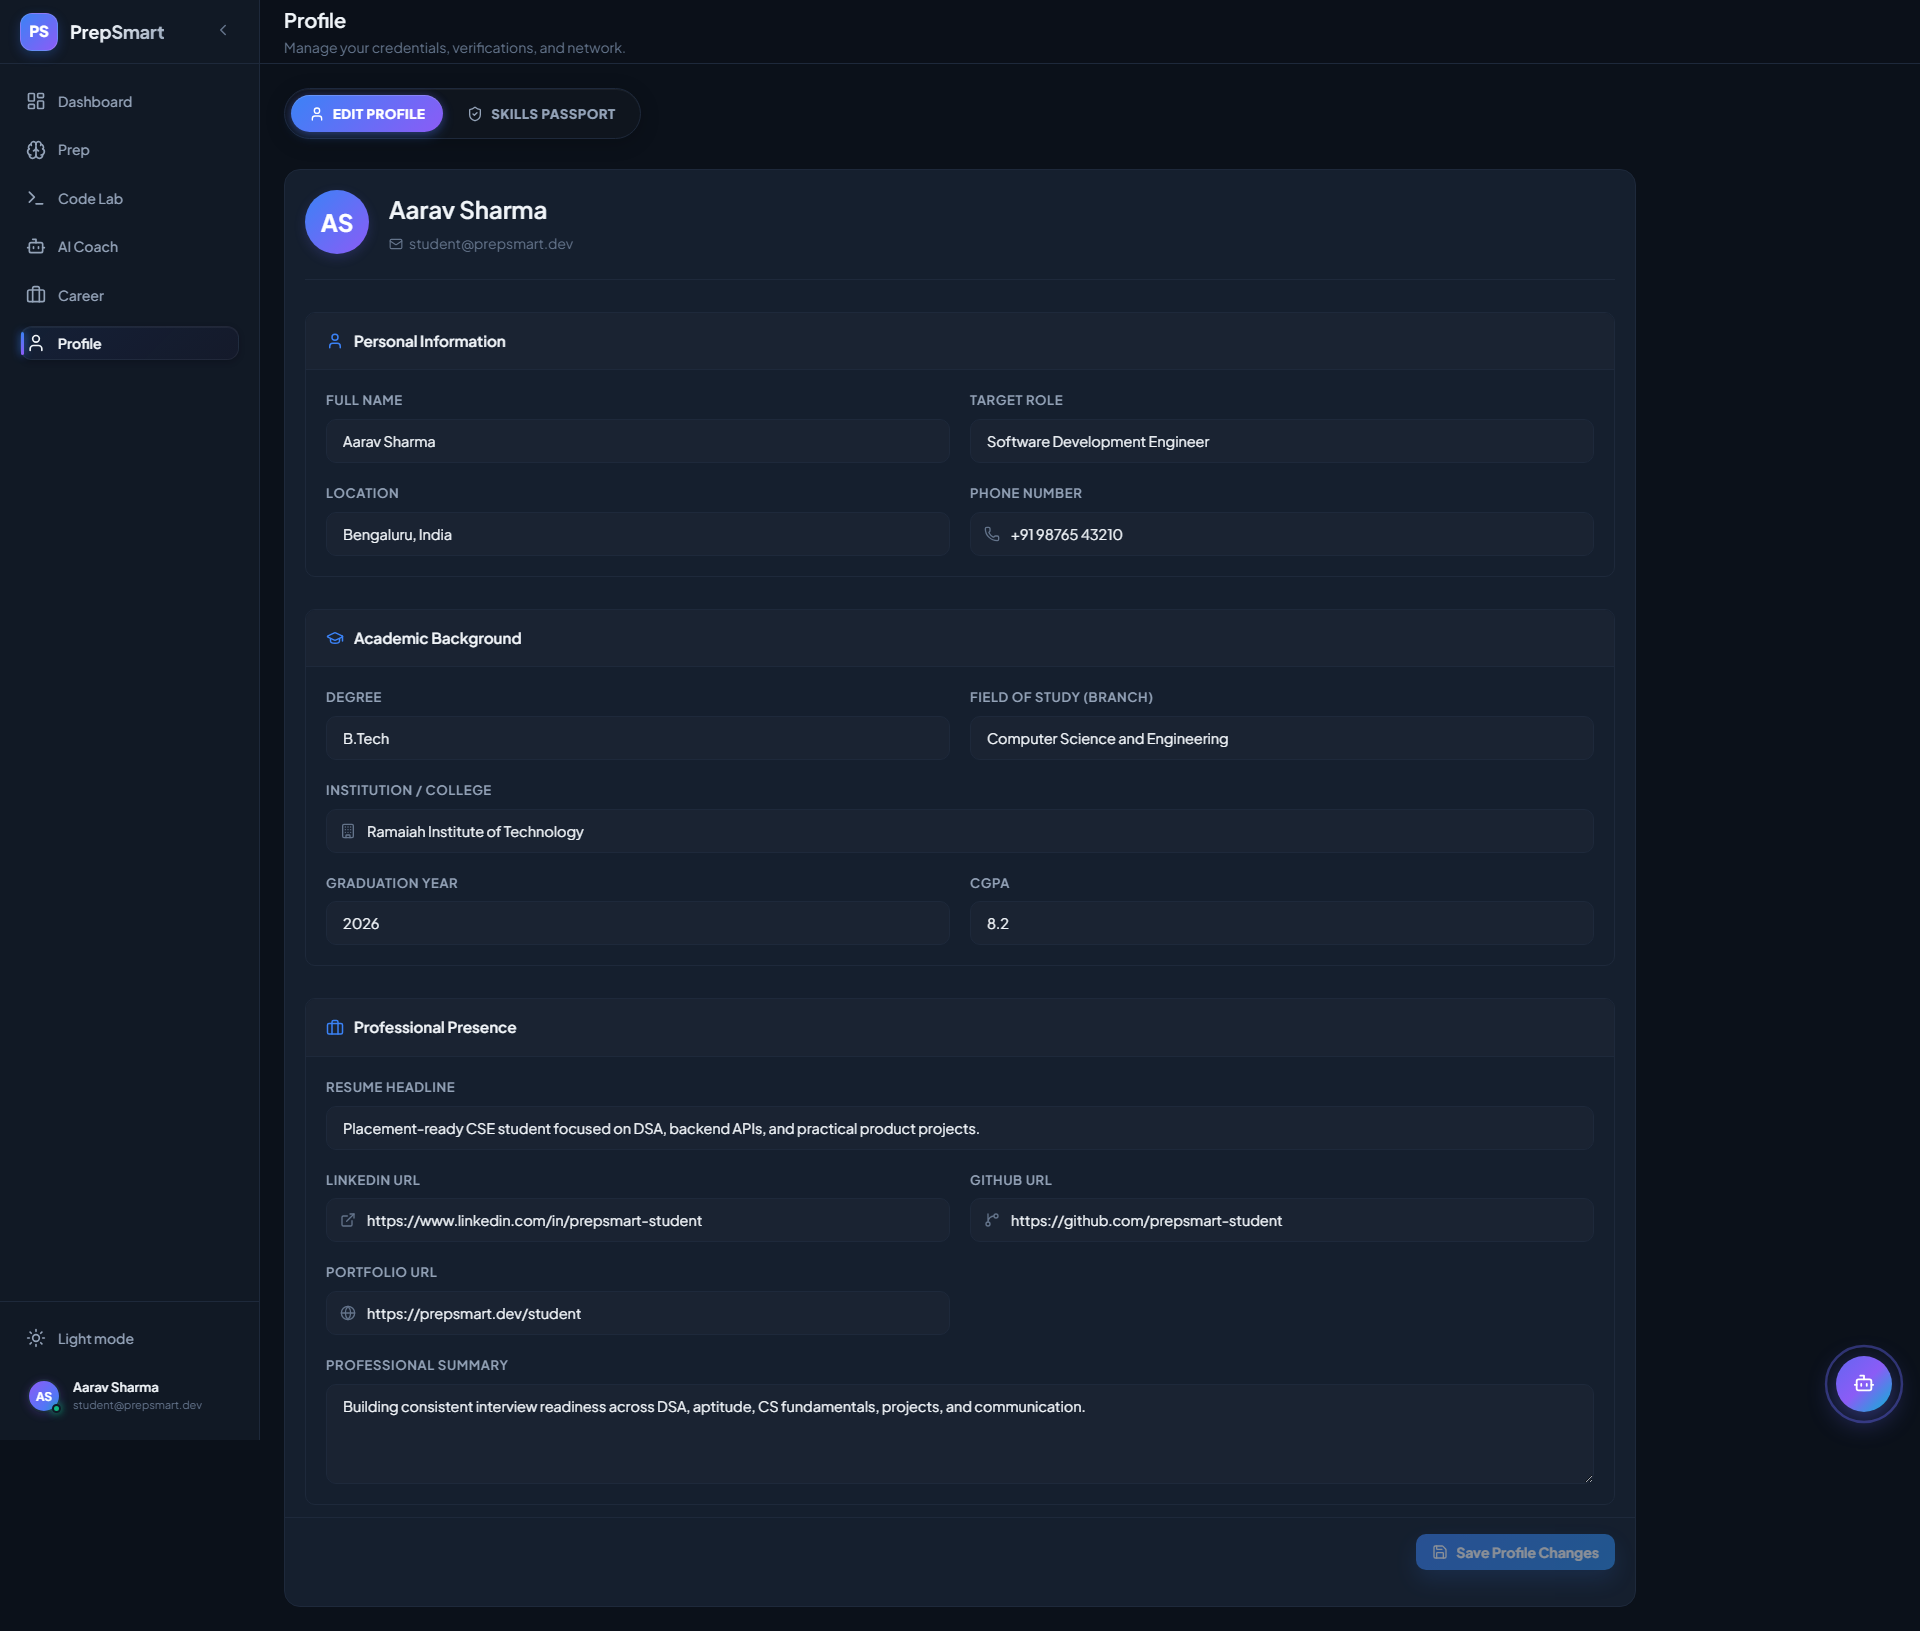
\includegraphics[width=0.95\textwidth]{Media/Chapter 5/profile_editor.png}
\caption{Profile Editor}
\label{fig:profile_editor}
\end{figure}

Figure~\ref{fig:profile_editor} illustrates the Profile Editor interface of PrepSmart. This page enables students to manage personal information, academic details, technical skills, target companies, career goals, and other profile-related information.

Users can update their profile whenever required, ensuring that the platform always maintains accurate information. The stored profile data is utilized by several modules, including dashboard analytics, company readiness evaluation, portfolio generation, and personalized placement recommendations.

The interface follows a simple and responsive design, allowing users to efficiently manage their information through organized input forms.

\subsubsection*{Major Features}

\begin{itemize}

\item Personal information management.

\item Academic profile management.

\item Technical skills management.

\item Target company preferences.

\item Career goal management.

\item Integration with placement analytics.

\end{itemize}

\subsection{Skills Passport}

The Skills Passport provides students with a consolidated view of their technical competencies, placement readiness, and overall employability. It summarizes learning progress and performance collected from different modules of the platform.

\begin{figure}[H]
\centering
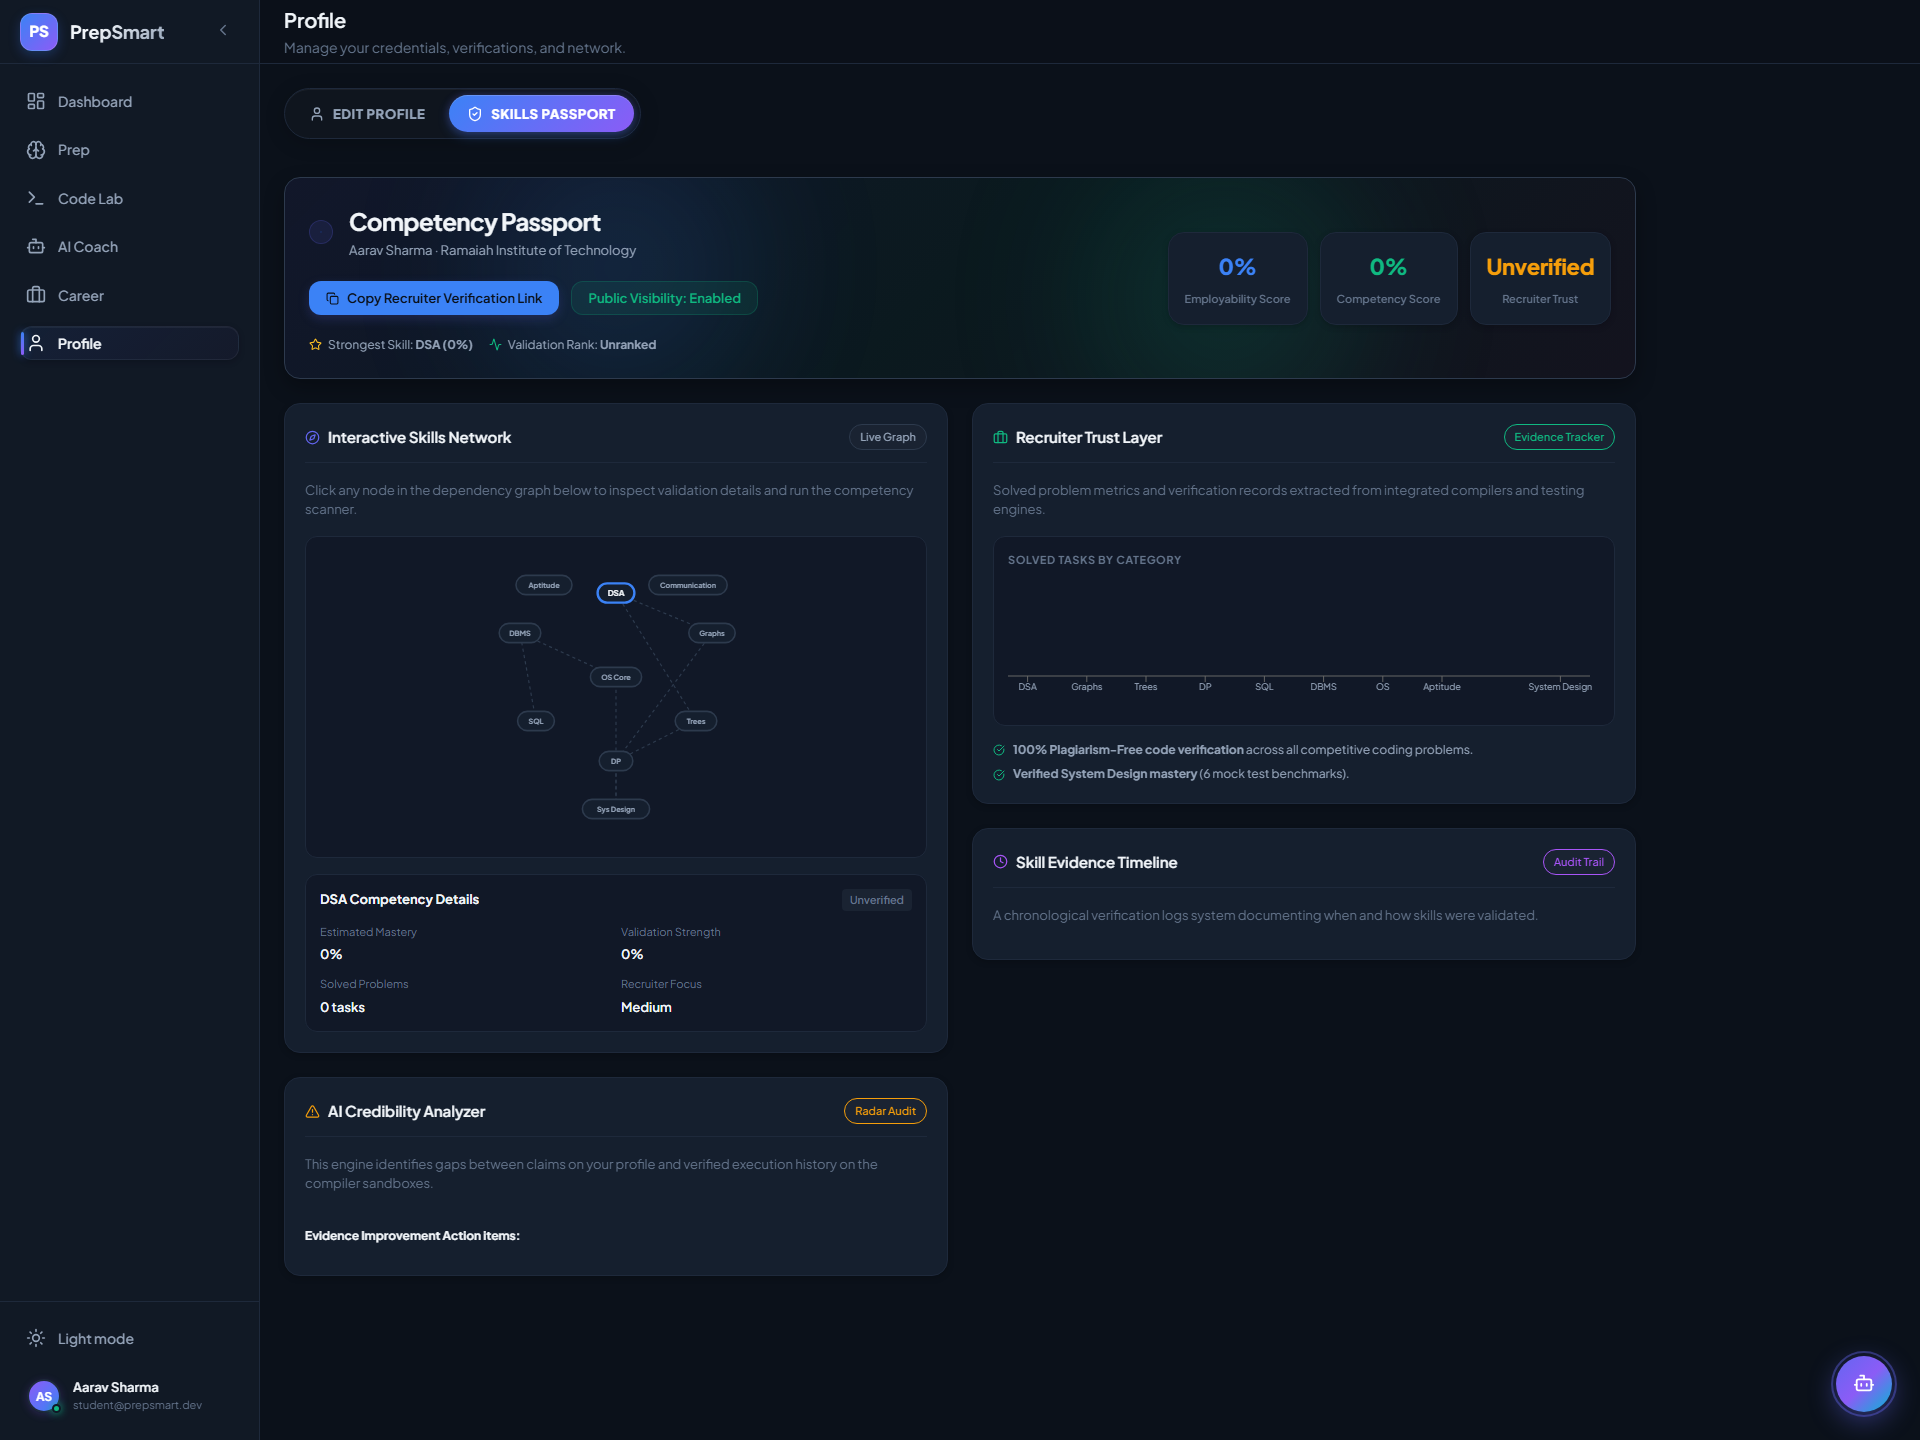
\includegraphics[width=0.95\textwidth]{Media/Chapter 5/skills_passport.png}
\caption{Skills Passport}
\label{fig:skills_passport}
\end{figure}

Figure~\ref{fig:skills_passport} presents the Skills Passport generated by PrepSmart. The interface summarizes the student's placement preparation using various performance indicators such as technical competency, coding activity, interview readiness, completed learning tracks, and overall employability.

The Skills Passport is generated automatically from the student's learning history and requires minimal manual intervention. It provides students with a comprehensive overview of their current preparation status while helping recruiters and placement coordinators understand the student's technical capabilities.

The information displayed within the Skills Passport is continuously updated whenever the student completes additional learning activities or assessments.

\subsubsection*{Major Features}

\begin{itemize}

\item Automatic employability profile generation.

\item Technical competency visualization.

\item Placement readiness indicators.

\item Coding performance summary.

\item Interview readiness tracking.

\item Continuous automatic updates.

\end{itemize}

\section{Shared Profiles}

PrepSmart enables students to share their professional profiles with recruiters, placement coordinators, and other external users through secure public links. The Shared Profiles module allows selected information to be viewed without exposing confidential user data.

\subsection{Shared Passport}

The Shared Passport interface presents a publicly accessible version of the student's Skills Passport that can be shared with recruiters and placement coordinators.

\begin{figure}[H]
\centering
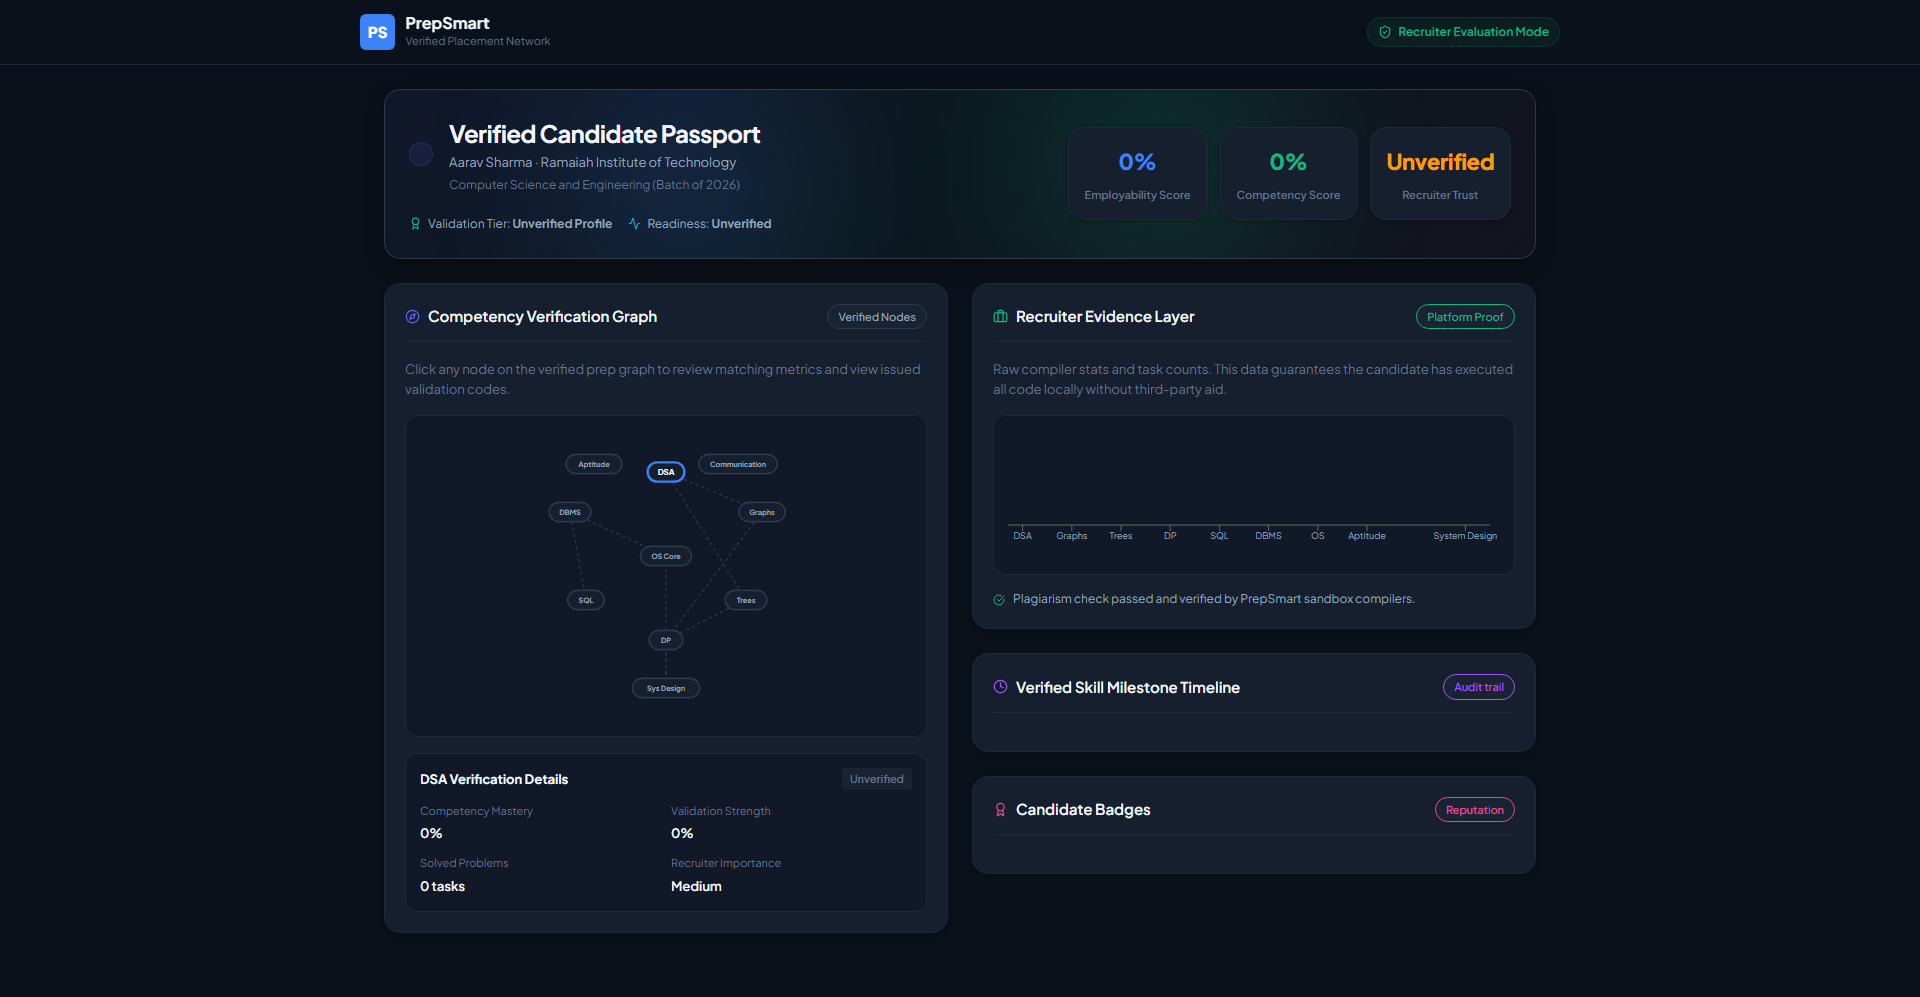
\includegraphics[width=0.95\textwidth]{Media/Chapter 5/shared_passport.png}
\caption{Shared Skills Passport}
\label{fig:shared_passport}
\end{figure}

Figure~\ref{fig:shared_passport} illustrates the publicly shared Skills Passport. This page presents selected placement readiness information while protecting confidential account details.

Recruiters can review technical competencies, learning progress, interview readiness, and employability indicators without requiring direct access to the student's PrepSmart account.

\subsection{Shared Portfolio}

The Shared Portfolio enables students to publicly showcase their projects, technical skills, certifications, and professional achievements using a dedicated shareable webpage.

\begin{figure}[H]
\centering
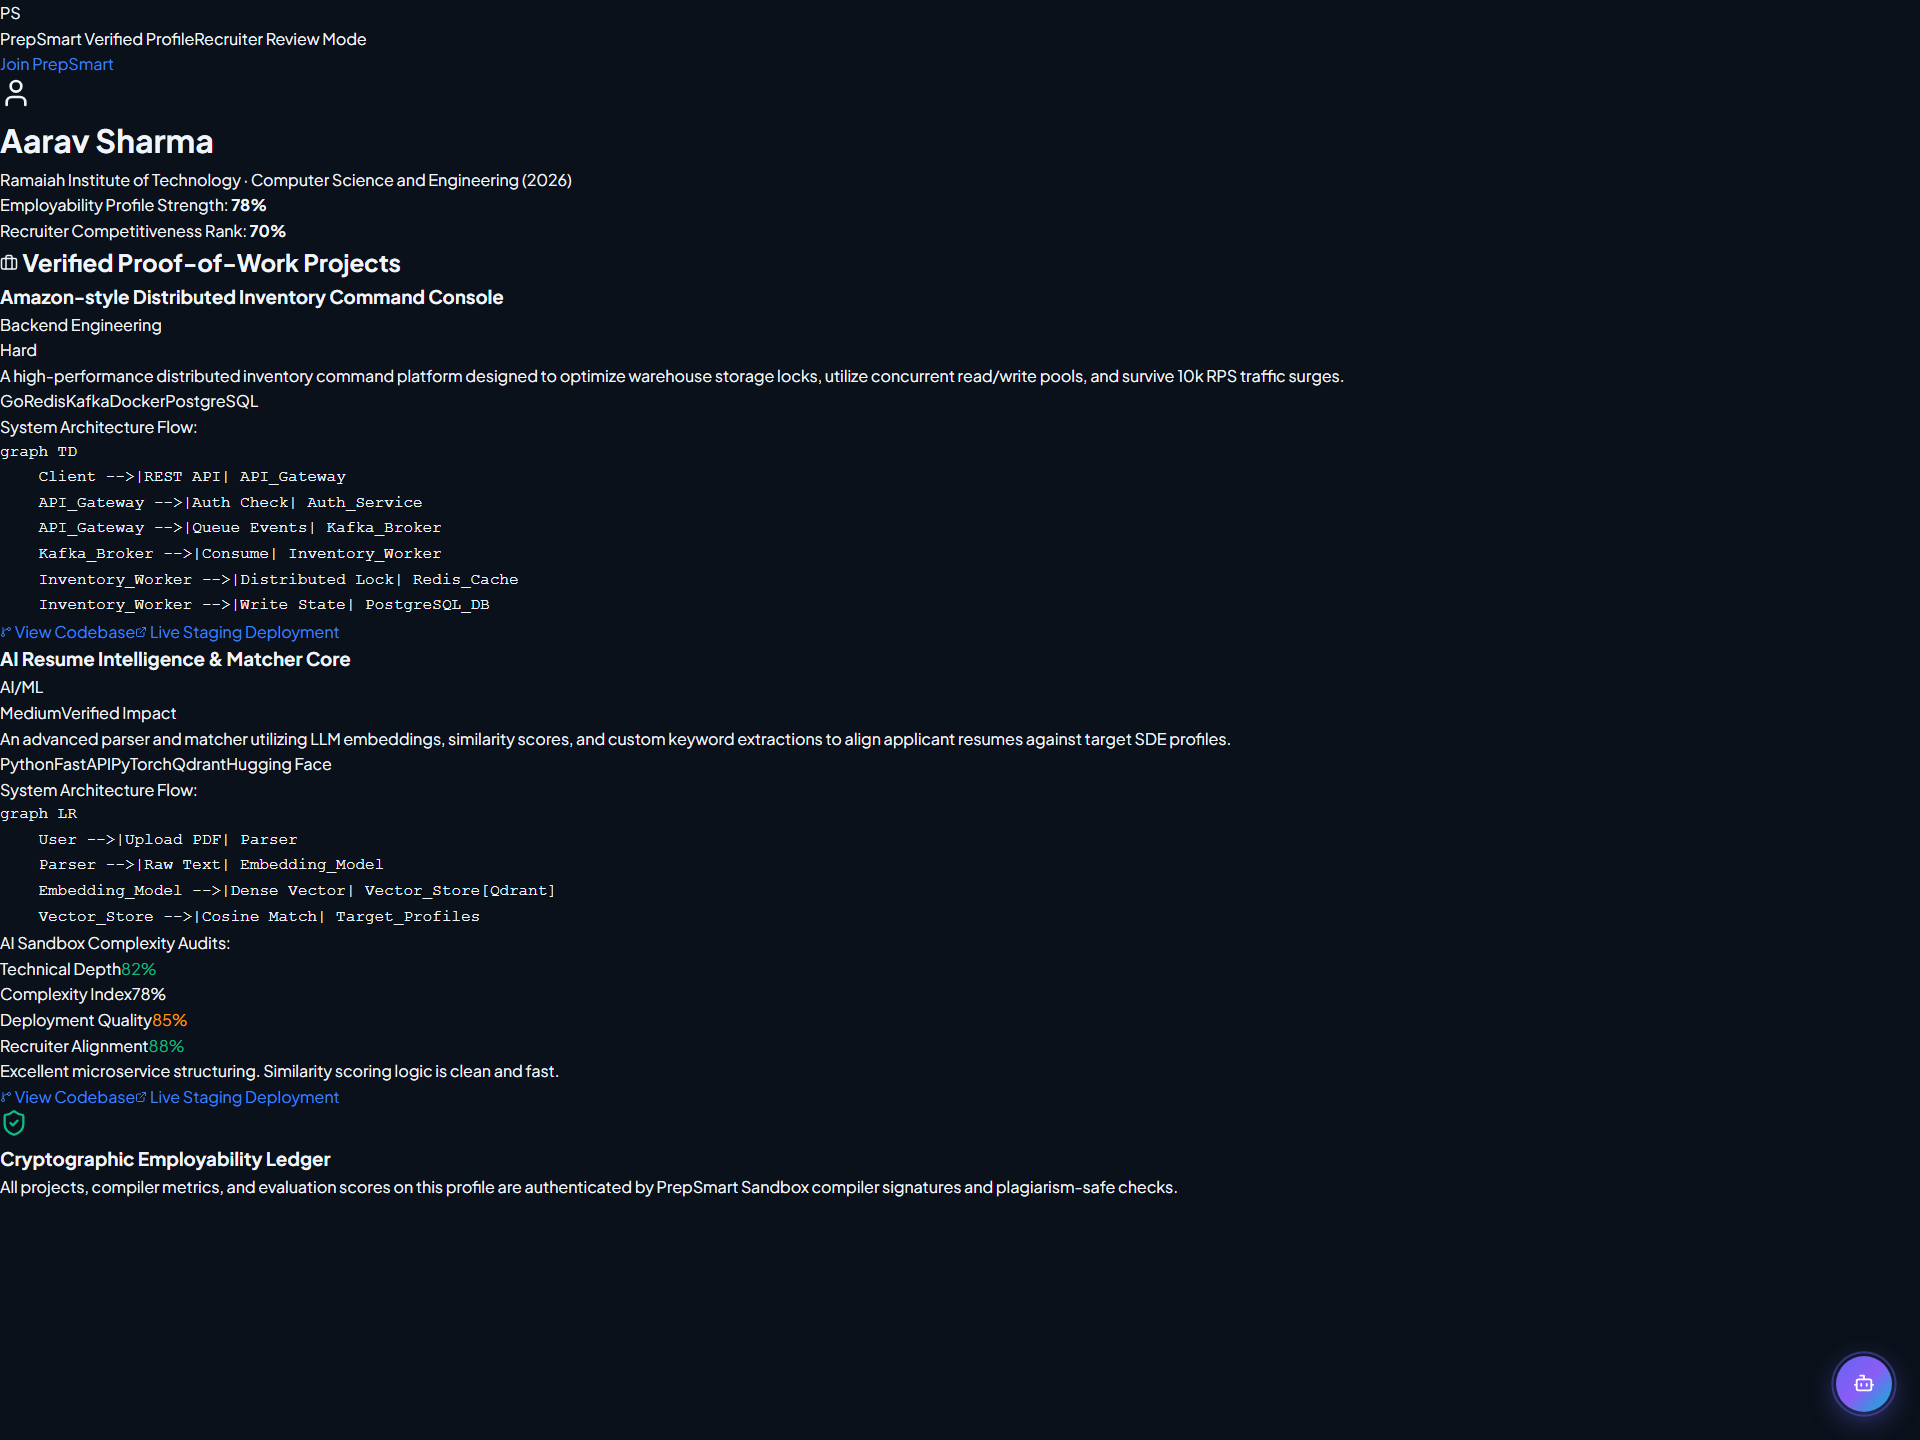
\includegraphics[width=0.95\textwidth]{Media/Chapter 5/shared_portfolio.png}
\caption{Shared Portfolio}
\label{fig:shared_portfolio}
\end{figure}

Figure~\ref{fig:shared_portfolio} presents the publicly accessible portfolio generated by PrepSmart. The page organizes the student's projects, skills, certifications, academic profile, and other professional achievements into a structured format suitable for recruiters.

The portfolio is generated dynamically from information already stored within the platform, eliminating the need for students to manually create separate portfolio websites.

\subsection*{Major Features of Shared Profiles}

\begin{itemize}

\item Public profile sharing.

\item Secure access through unique links.

\item Recruiter-friendly presentation.

\item Dynamic profile generation.

\item Automatic synchronization with user data.

\item Privacy protection for confidential information.

\end{itemize}

\section{Analytics Dashboard}

The Analytics Dashboard provides students with a detailed analysis of their placement preparation by presenting various performance indicators and statistical visualizations. Unlike the main dashboard, which provides an overall summary, the analytics module focuses on detailed performance evaluation, enabling students to identify strengths, weaknesses, and improvement opportunities.

The interface continuously updates analytical information using data collected from learning activities, coding practice, mock tests, interview sessions, and company preparation modules.

\begin{figure}[H]
\centering
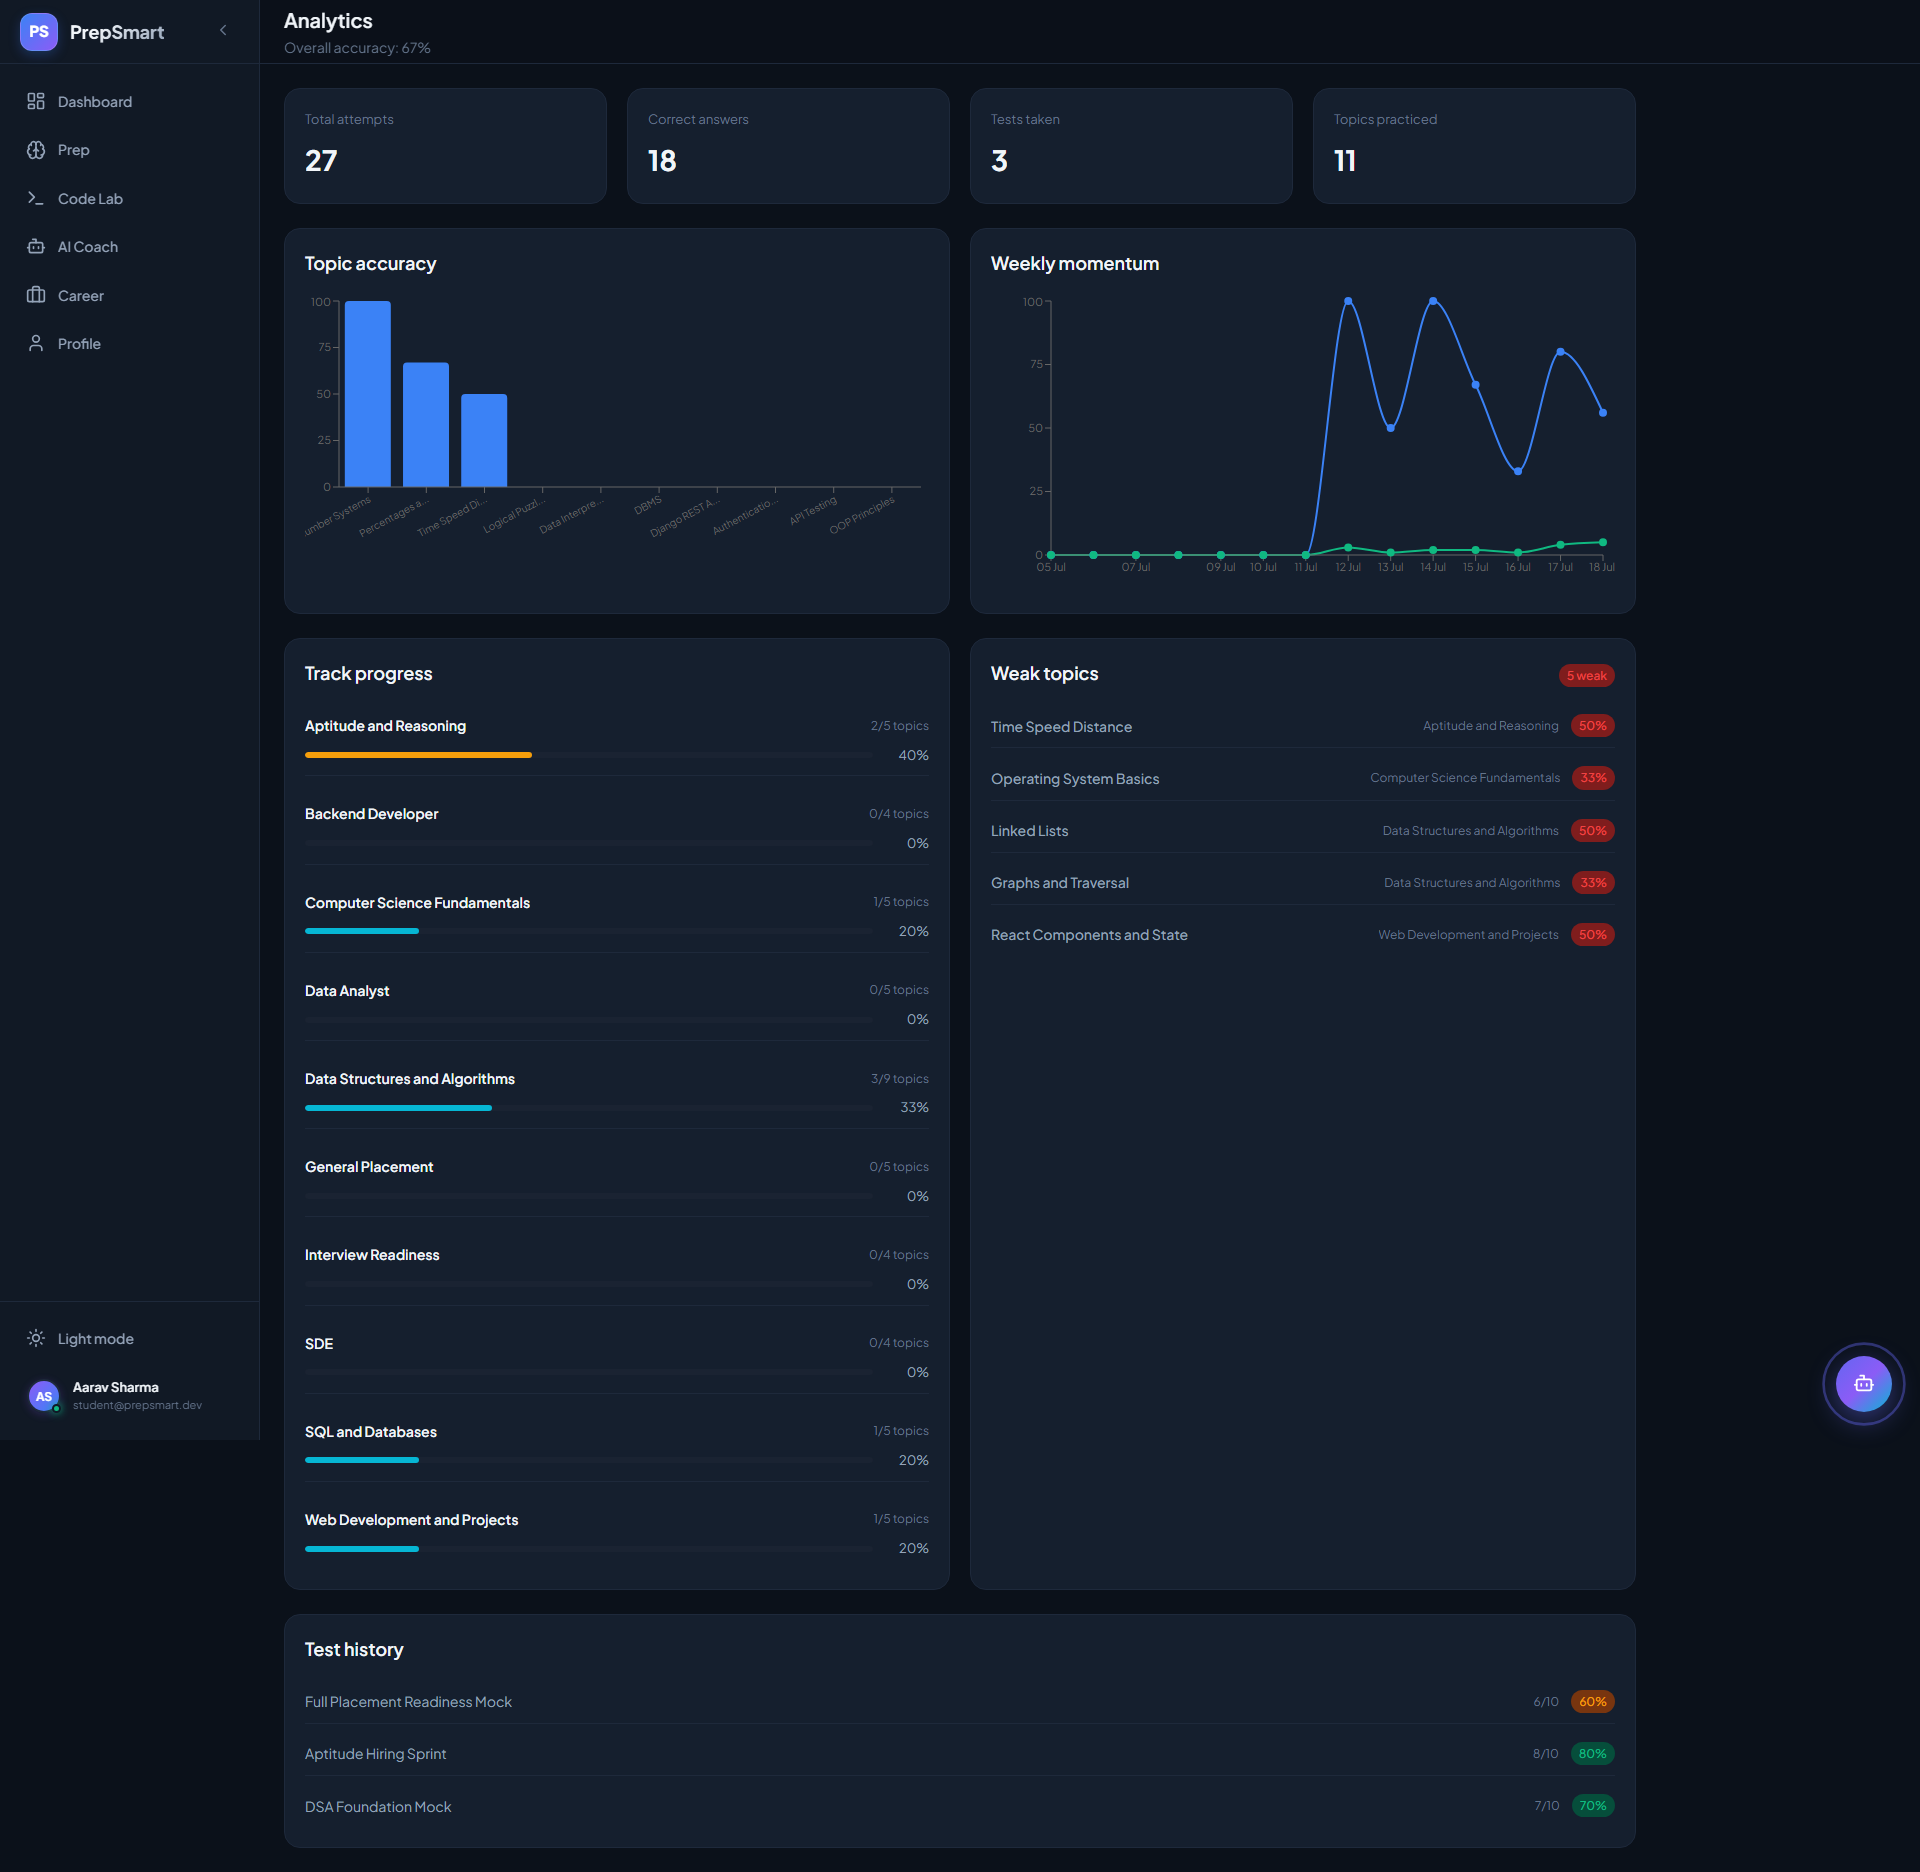
\includegraphics[width=0.95\textwidth]{Media/Chapter 5/analytics.png}
\caption{Analytics Dashboard}
\label{fig:analytics_dashboard}
\end{figure}

Figure~\ref{fig:analytics_dashboard} illustrates the Analytics Dashboard of PrepSmart. The page presents various statistical summaries and graphical representations that help students evaluate their overall preparation progress.

The dashboard displays information such as topic completion percentages, coding activity, quiz accuracy, interview performance, company readiness, and learning trends. Interactive charts and progress indicators simplify the interpretation of performance data and enable students to identify areas requiring additional attention.

Since the displayed information is generated dynamically from the backend database, students always receive up-to-date analytical insights based on their latest activities.

\subsection*{Major Features}

\begin{itemize}

\item Learning progress analytics.

\item Coding performance statistics.

\item Interview performance analysis.

\item Company readiness visualization.

\item Interactive charts.

\item Real-time analytical updates.

\end{itemize}

\section{Settings}

The Settings module enables users to personalize their experience within the PrepSmart platform. It provides configuration options related to user preferences, application appearance, notification settings, and account management.

\begin{figure}[H]
\centering
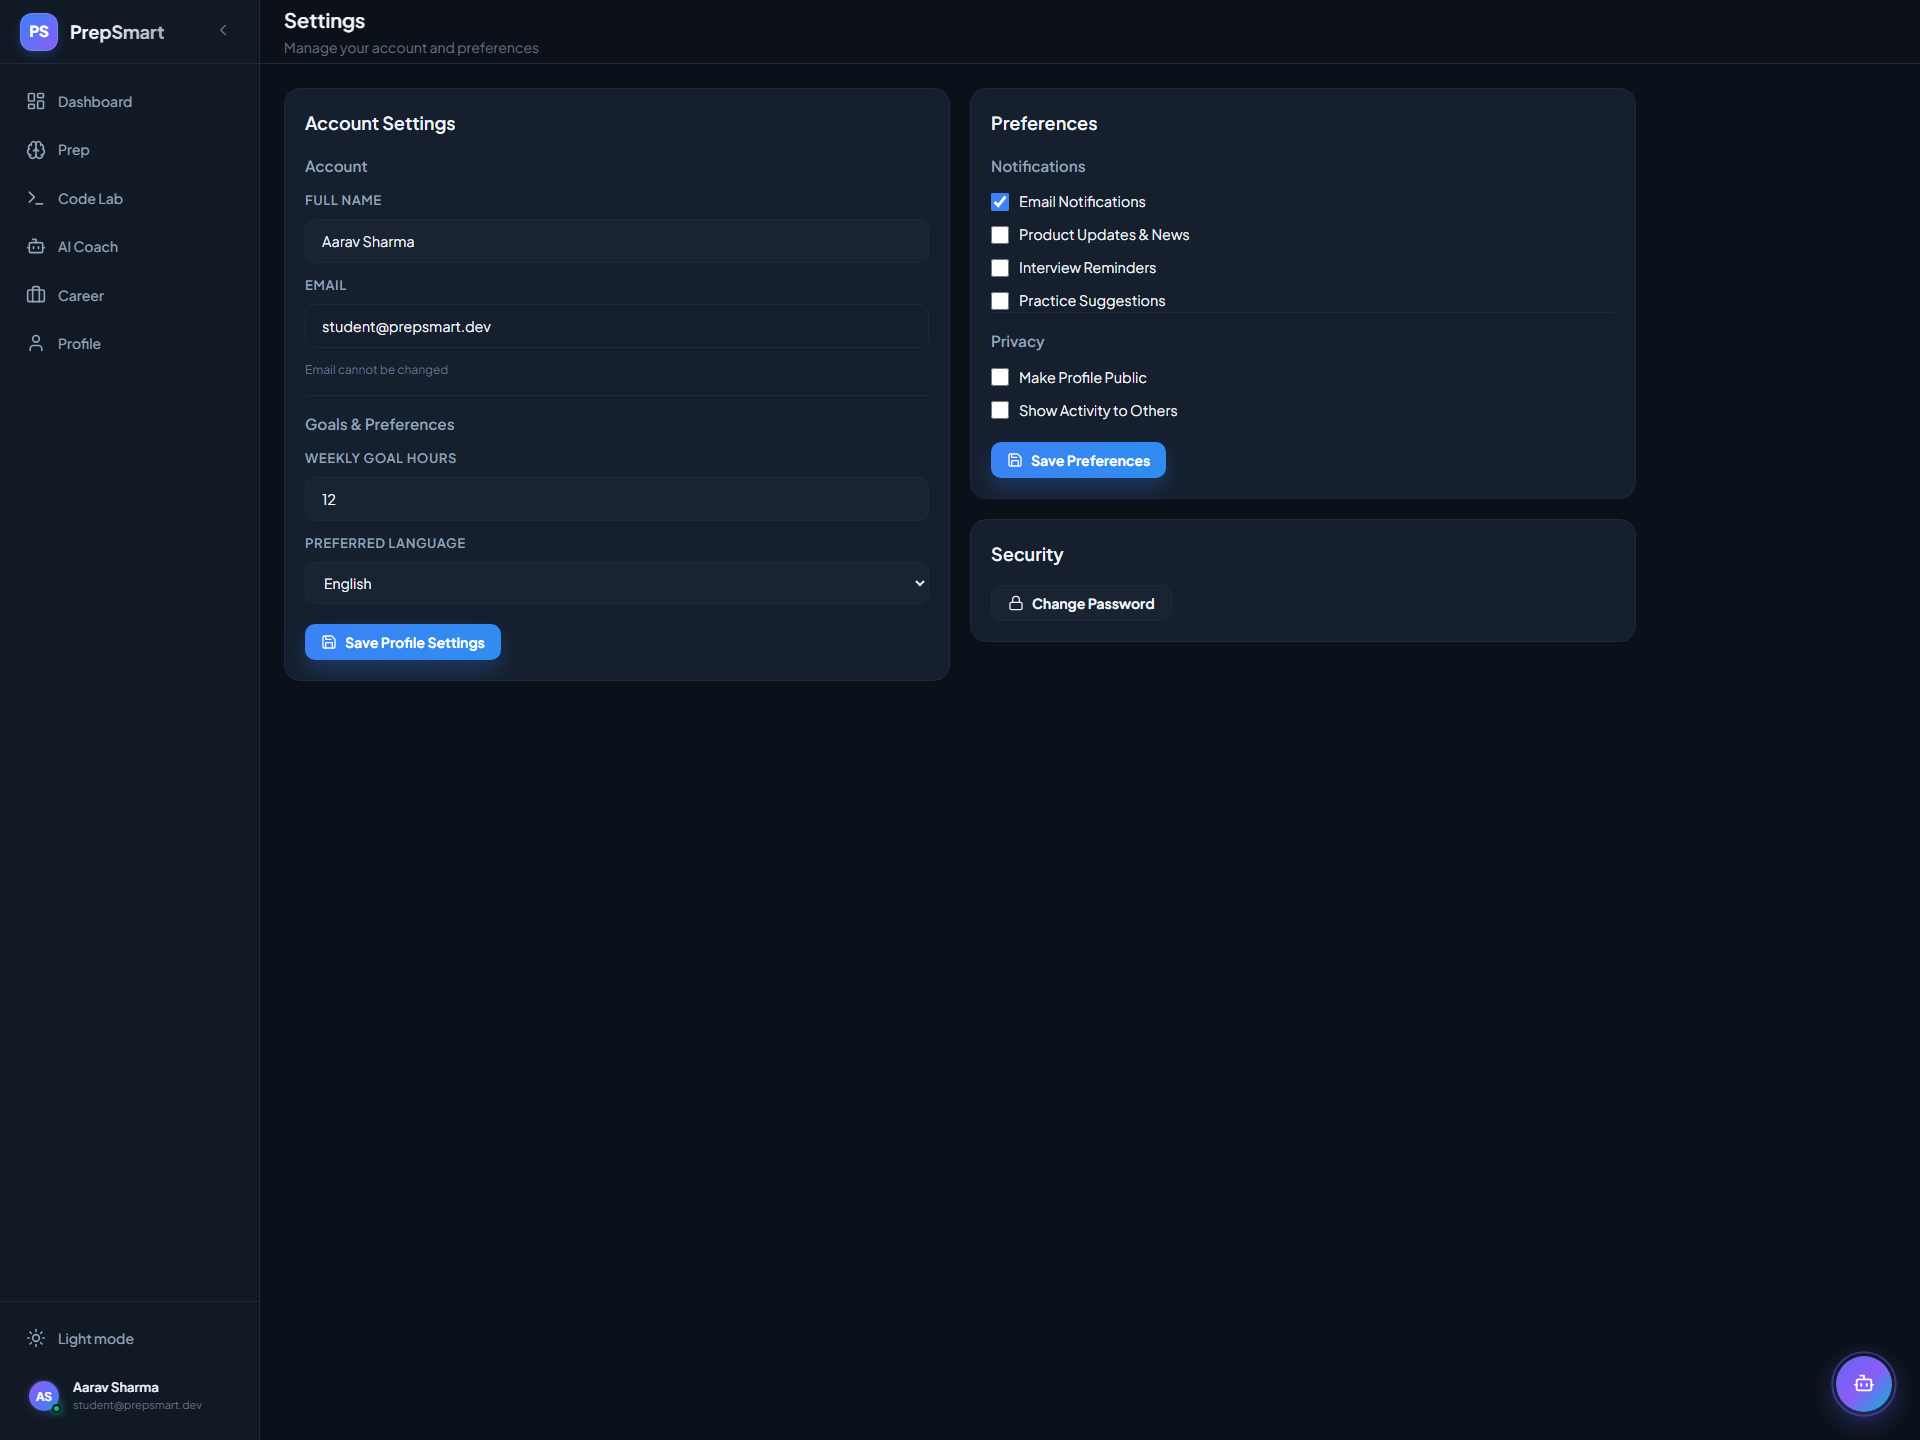
\includegraphics[width=0.95\textwidth]{Media/Chapter 5/settings.png}
\caption{Settings Interface}
\label{fig:settings}
\end{figure}

Figure~\ref{fig:settings} presents the Settings interface of PrepSmart. Through this page, users can manage their application preferences and personalize the overall user experience.

The interface provides options for updating account settings, adjusting application preferences, managing notifications, and configuring other personalized options. The responsive layout ensures that settings can be modified conveniently across different devices.

\subsection*{Major Features}

\begin{itemize}

\item User preference management.

\item Account settings.

\item Notification configuration.

\item Personalized application experience.

\item Responsive interface.

\end{itemize}

\section{Administration Module}

The Administration Module enables authorized administrators to manage the entire PrepSmart platform. Through the Django administrative interface, administrators can create, update, delete, and monitor different entities within the system. This centralized management simplifies content administration and ensures the smooth operation of the platform.

\subsection{User Management}

\begin{figure}[H]
\centering
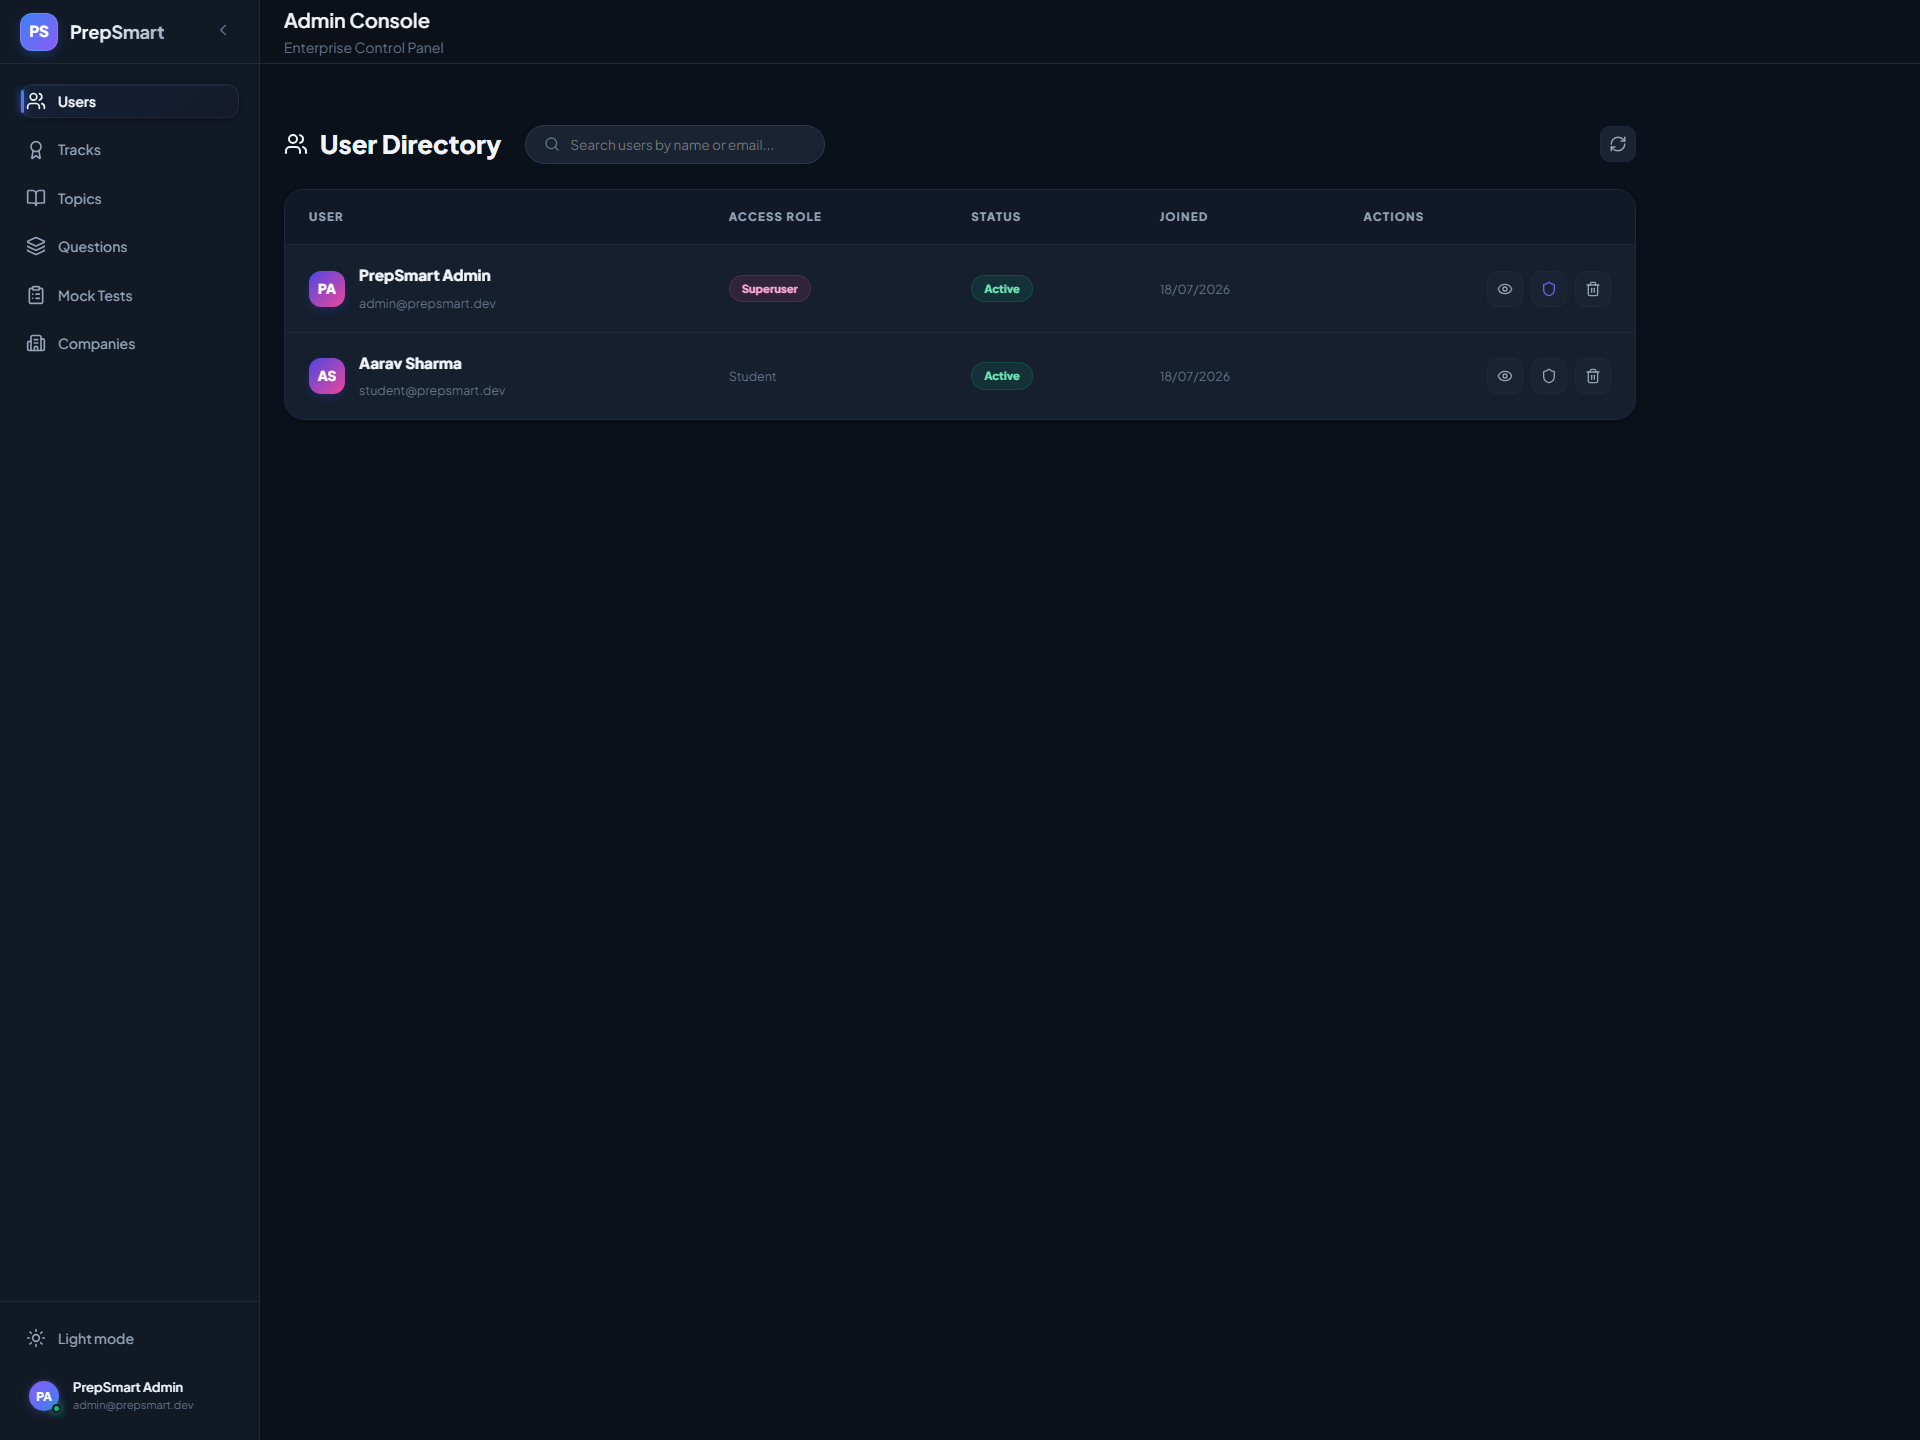
\includegraphics[width=0.90\textwidth]{Media/Chapter 5/admin_users.png}
\caption{Administration - User Management}
\label{fig:admin_users}
\end{figure}

The User Management interface enables administrators to monitor registered users, manage user accounts, update permissions, and perform administrative actions when required.

\subsection{Track Management}

\begin{figure}[H]
\centering
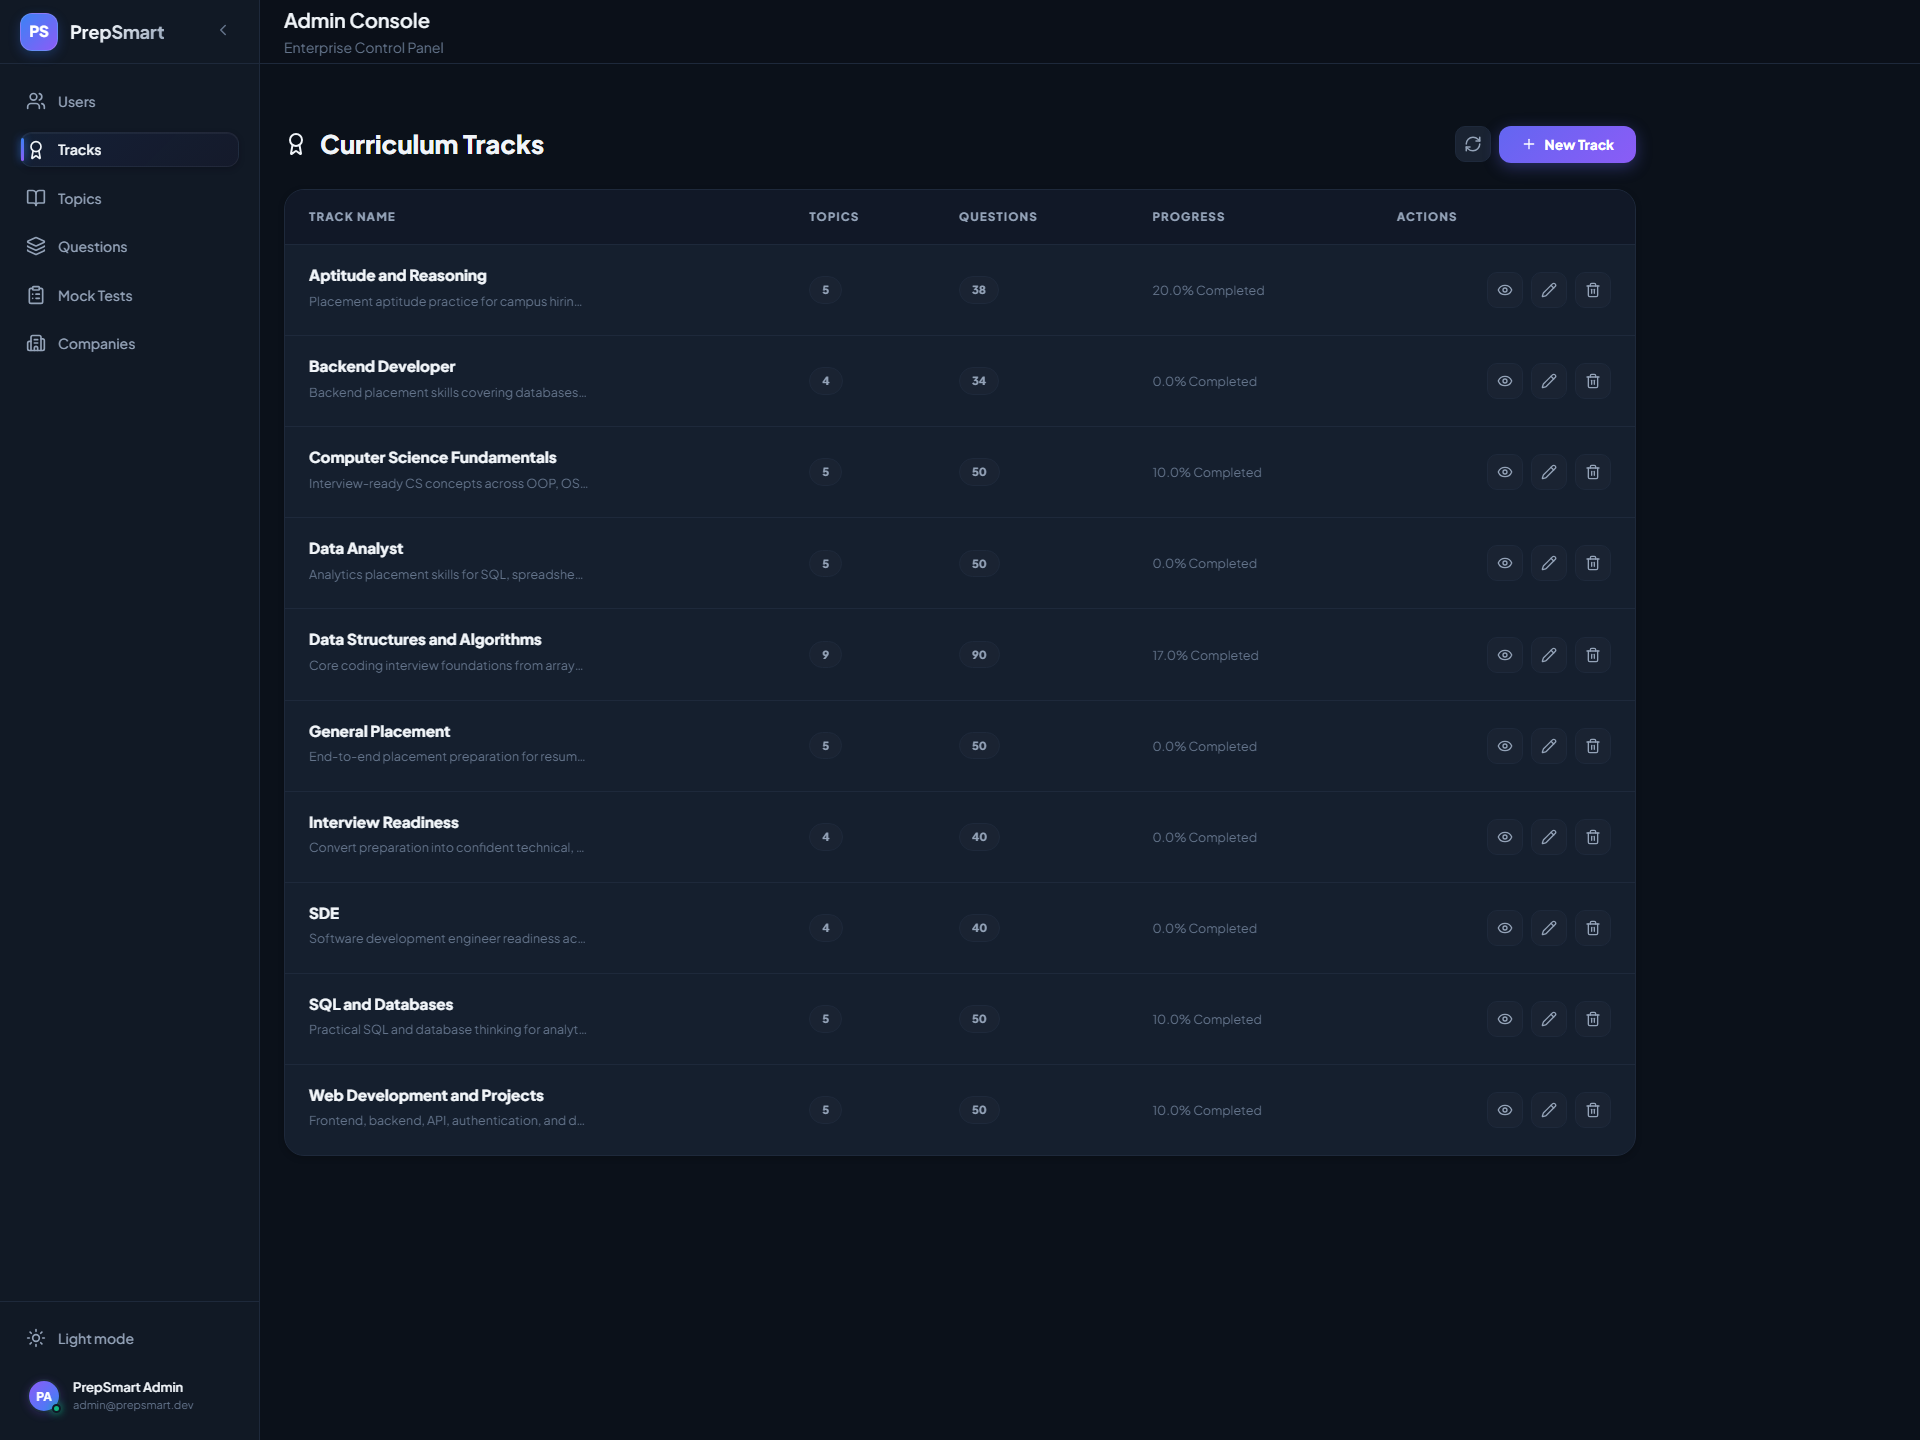
\includegraphics[width=0.90\textwidth]{Media/Chapter 5/admin_tracks.png}
\caption{Administration - Track Management}
\label{fig:admin_tracks}
\end{figure}

Administrators manage learning tracks through this interface by creating new preparation domains, updating existing tracks, and organizing educational content.

\subsection{Topic Management}

\begin{figure}[H]
\centering
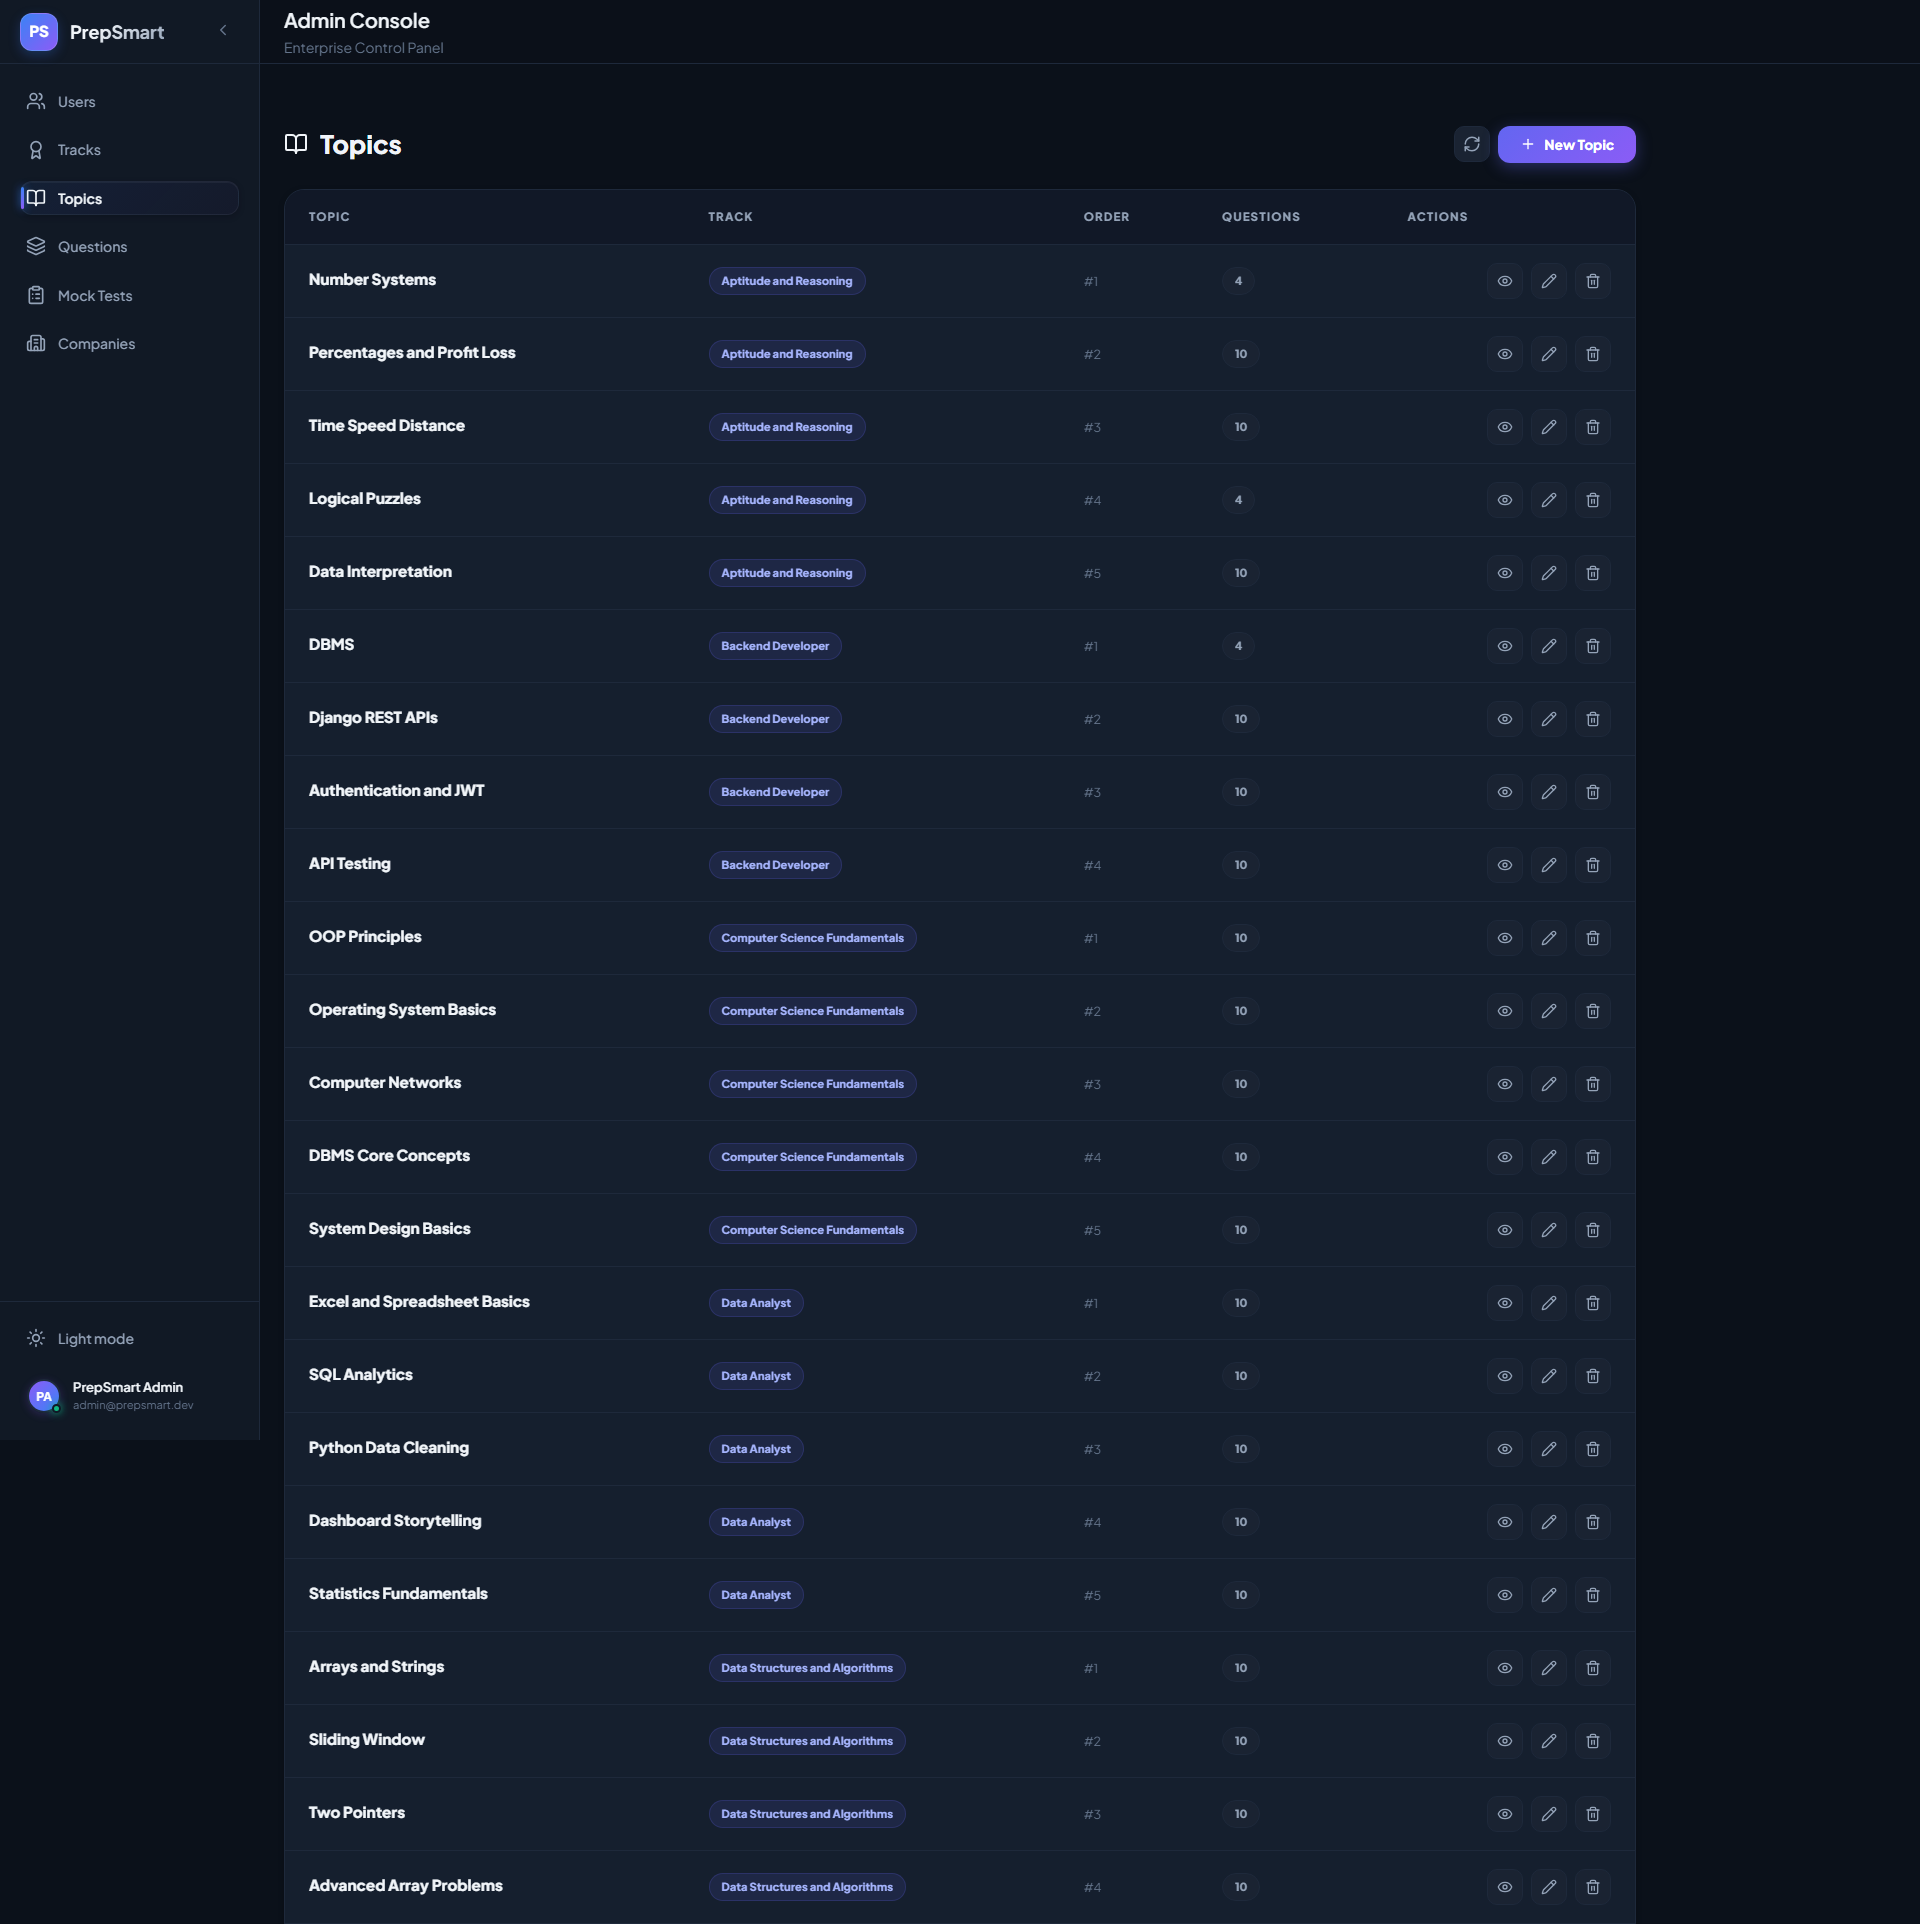
\includegraphics[width=0.90\textwidth]{Media/Chapter 5/admin_topics.png}
\caption{Administration - Topic Management}
\label{fig:admin_topics}
\end{figure}

The Topic Management interface enables administrators to organize individual learning topics, descriptions, prerequisites, and learning sequences used throughout the placement preparation module.

\subsection{Question Management}

\begin{figure}[H]
\centering
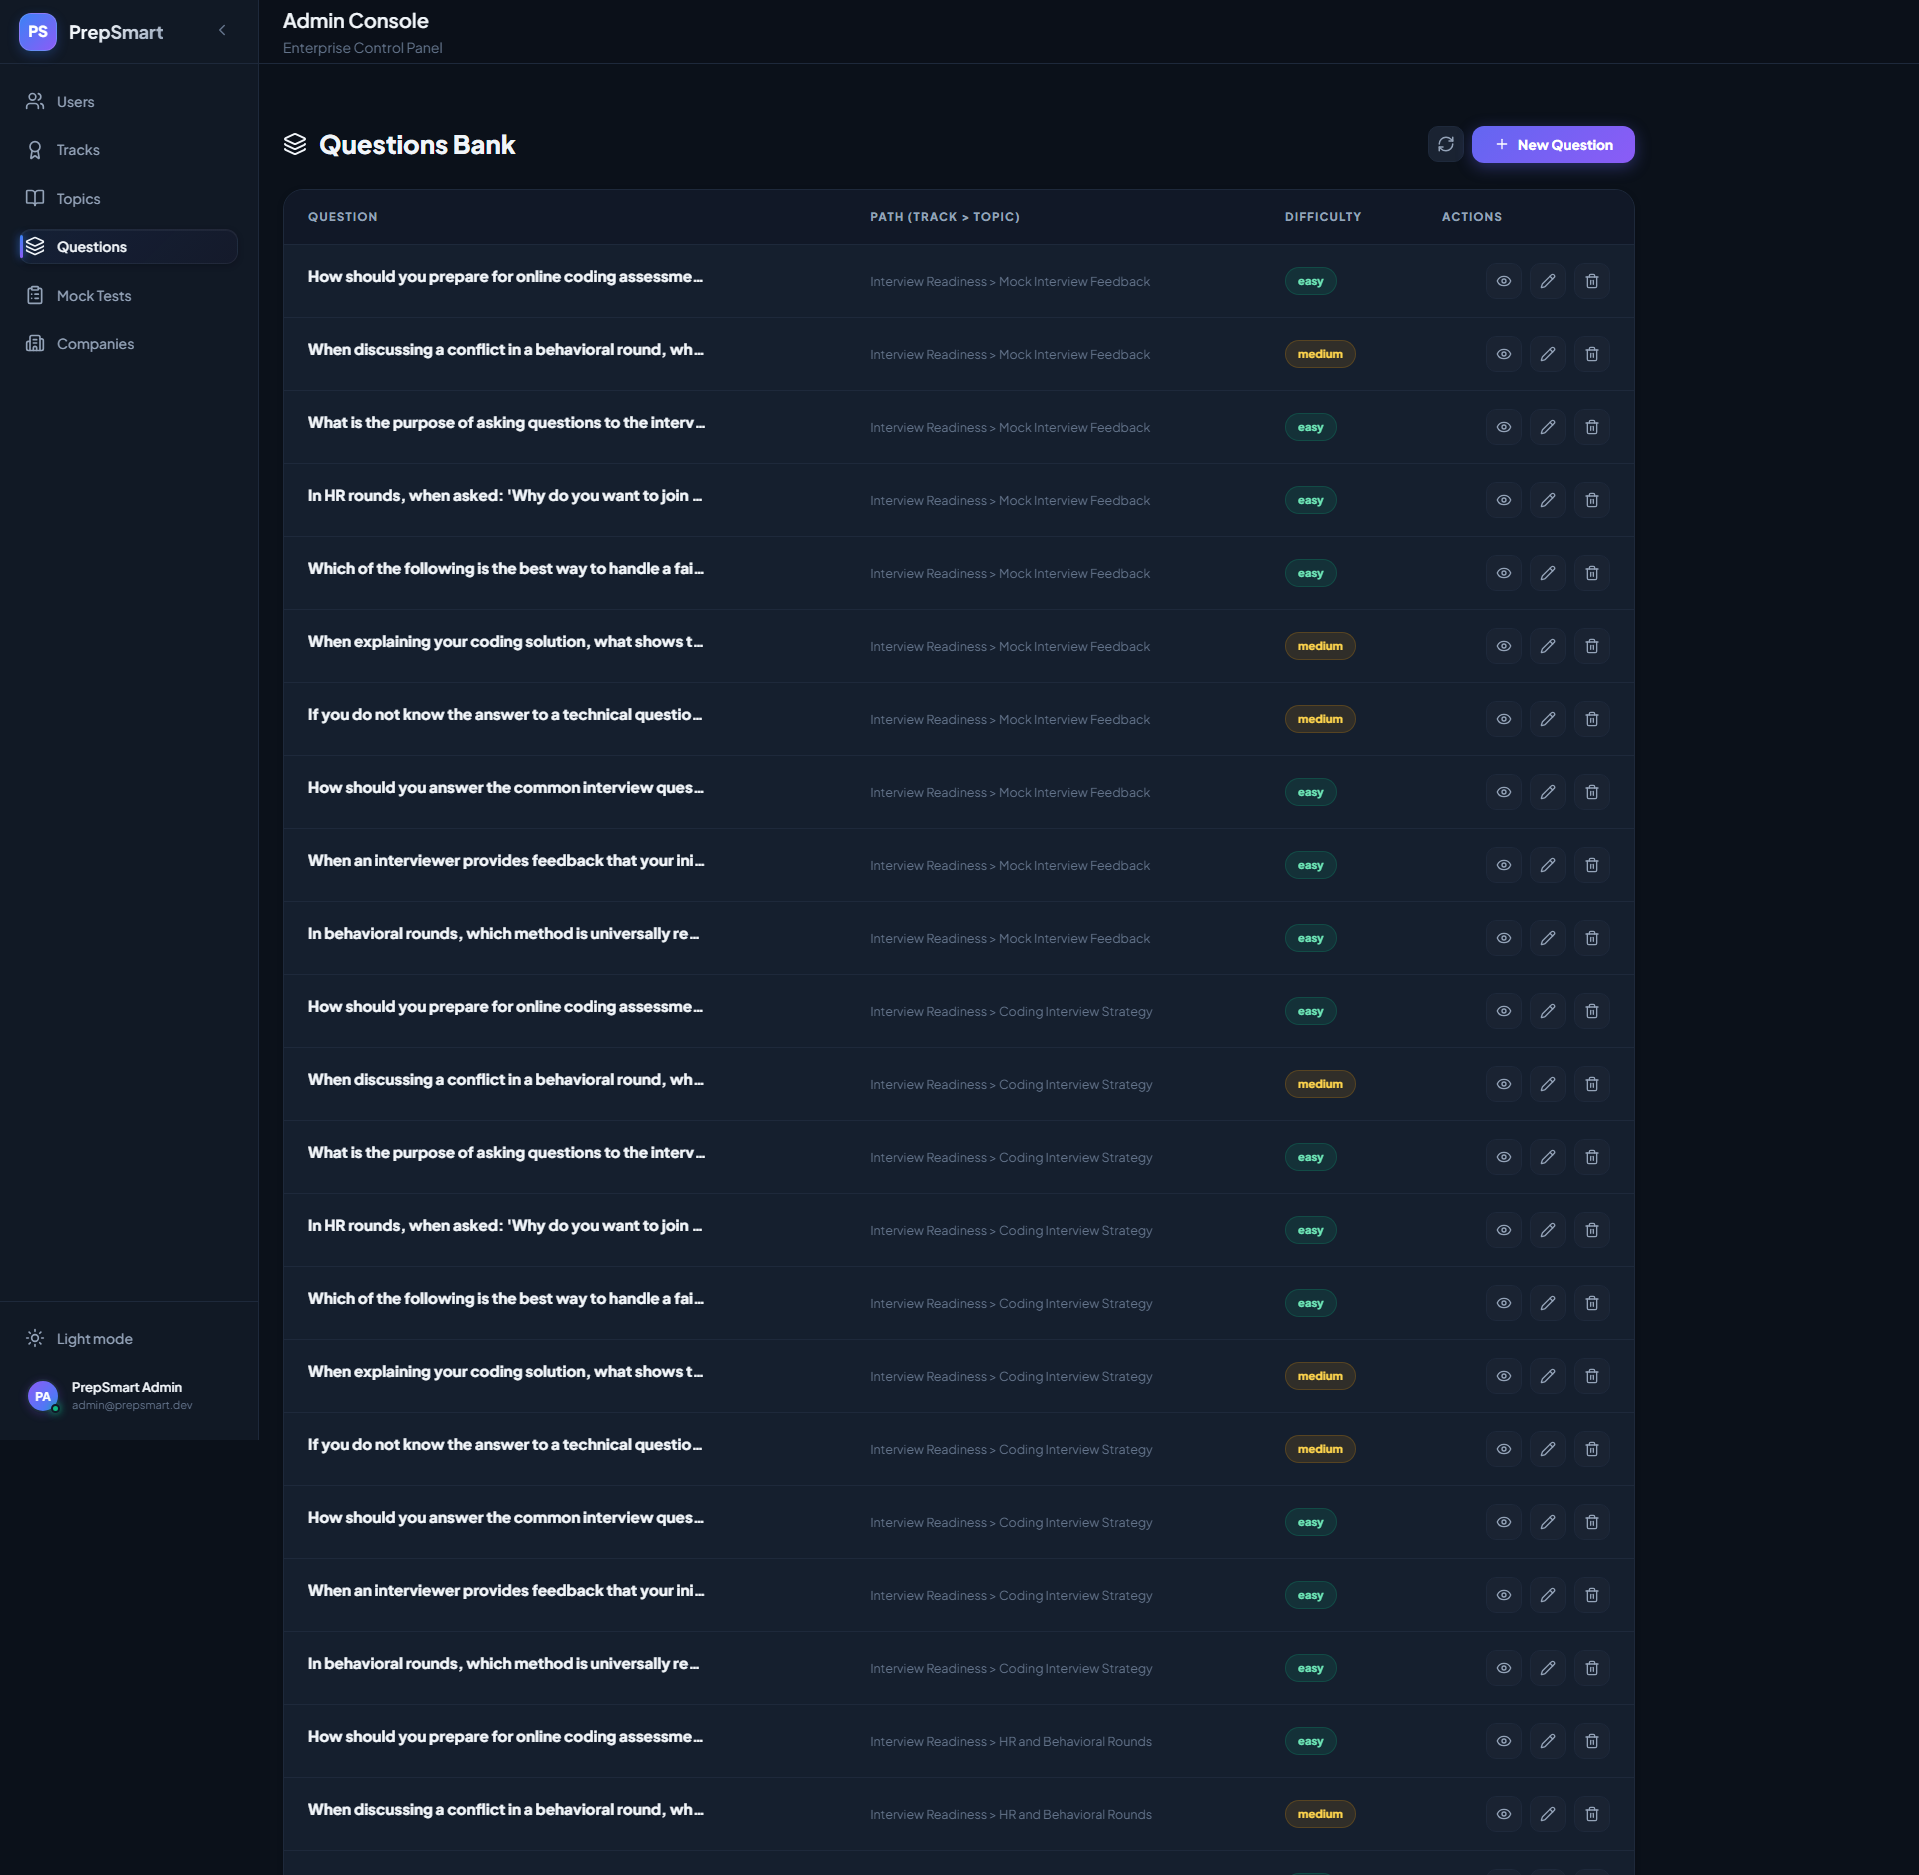
\includegraphics[width=0.90\textwidth]{Media/Chapter 5/admin_questions.png}
\caption{Administration - Question Management}
\label{fig:admin_questions}
\end{figure}

Administrators can create, modify, and maintain multiple-choice questions used in quizzes, assessments, and mock tests through this interface.

\subsection{Test Management}

\begin{figure}[H]
\centering
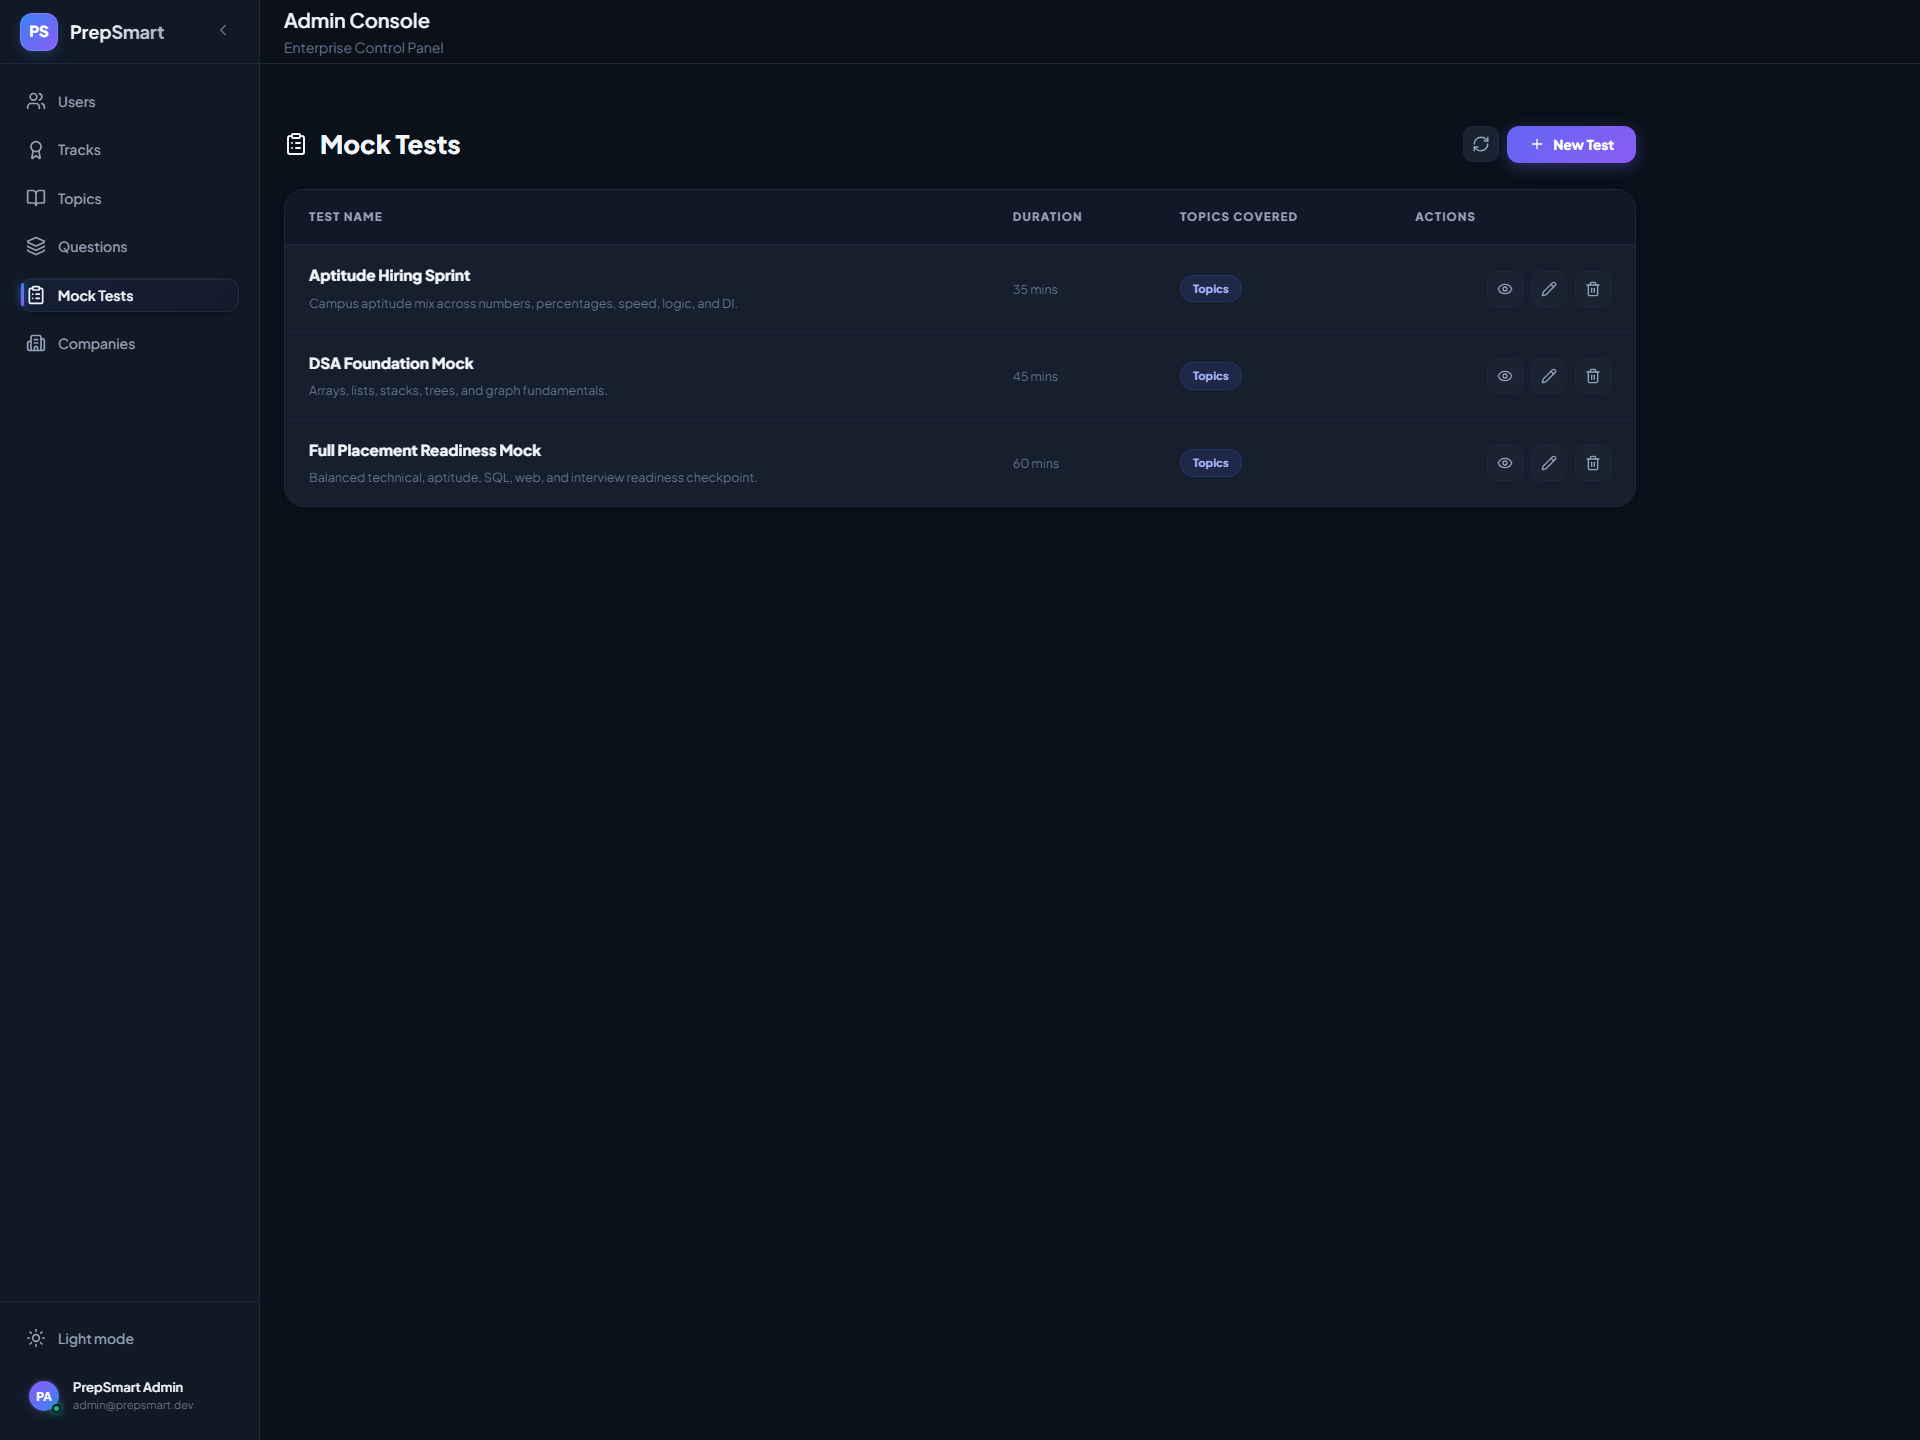
\includegraphics[width=0.90\textwidth]{Media/Chapter 5/admin_tests.png}
\caption{Administration - Test Management}
\label{fig:admin_tests}
\end{figure}

The Test Management interface allows administrators to configure mock tests, associate questions with assessments, and manage evaluation content for placement preparation.

\subsection{Company Management}

\begin{figure}[H]
\centering
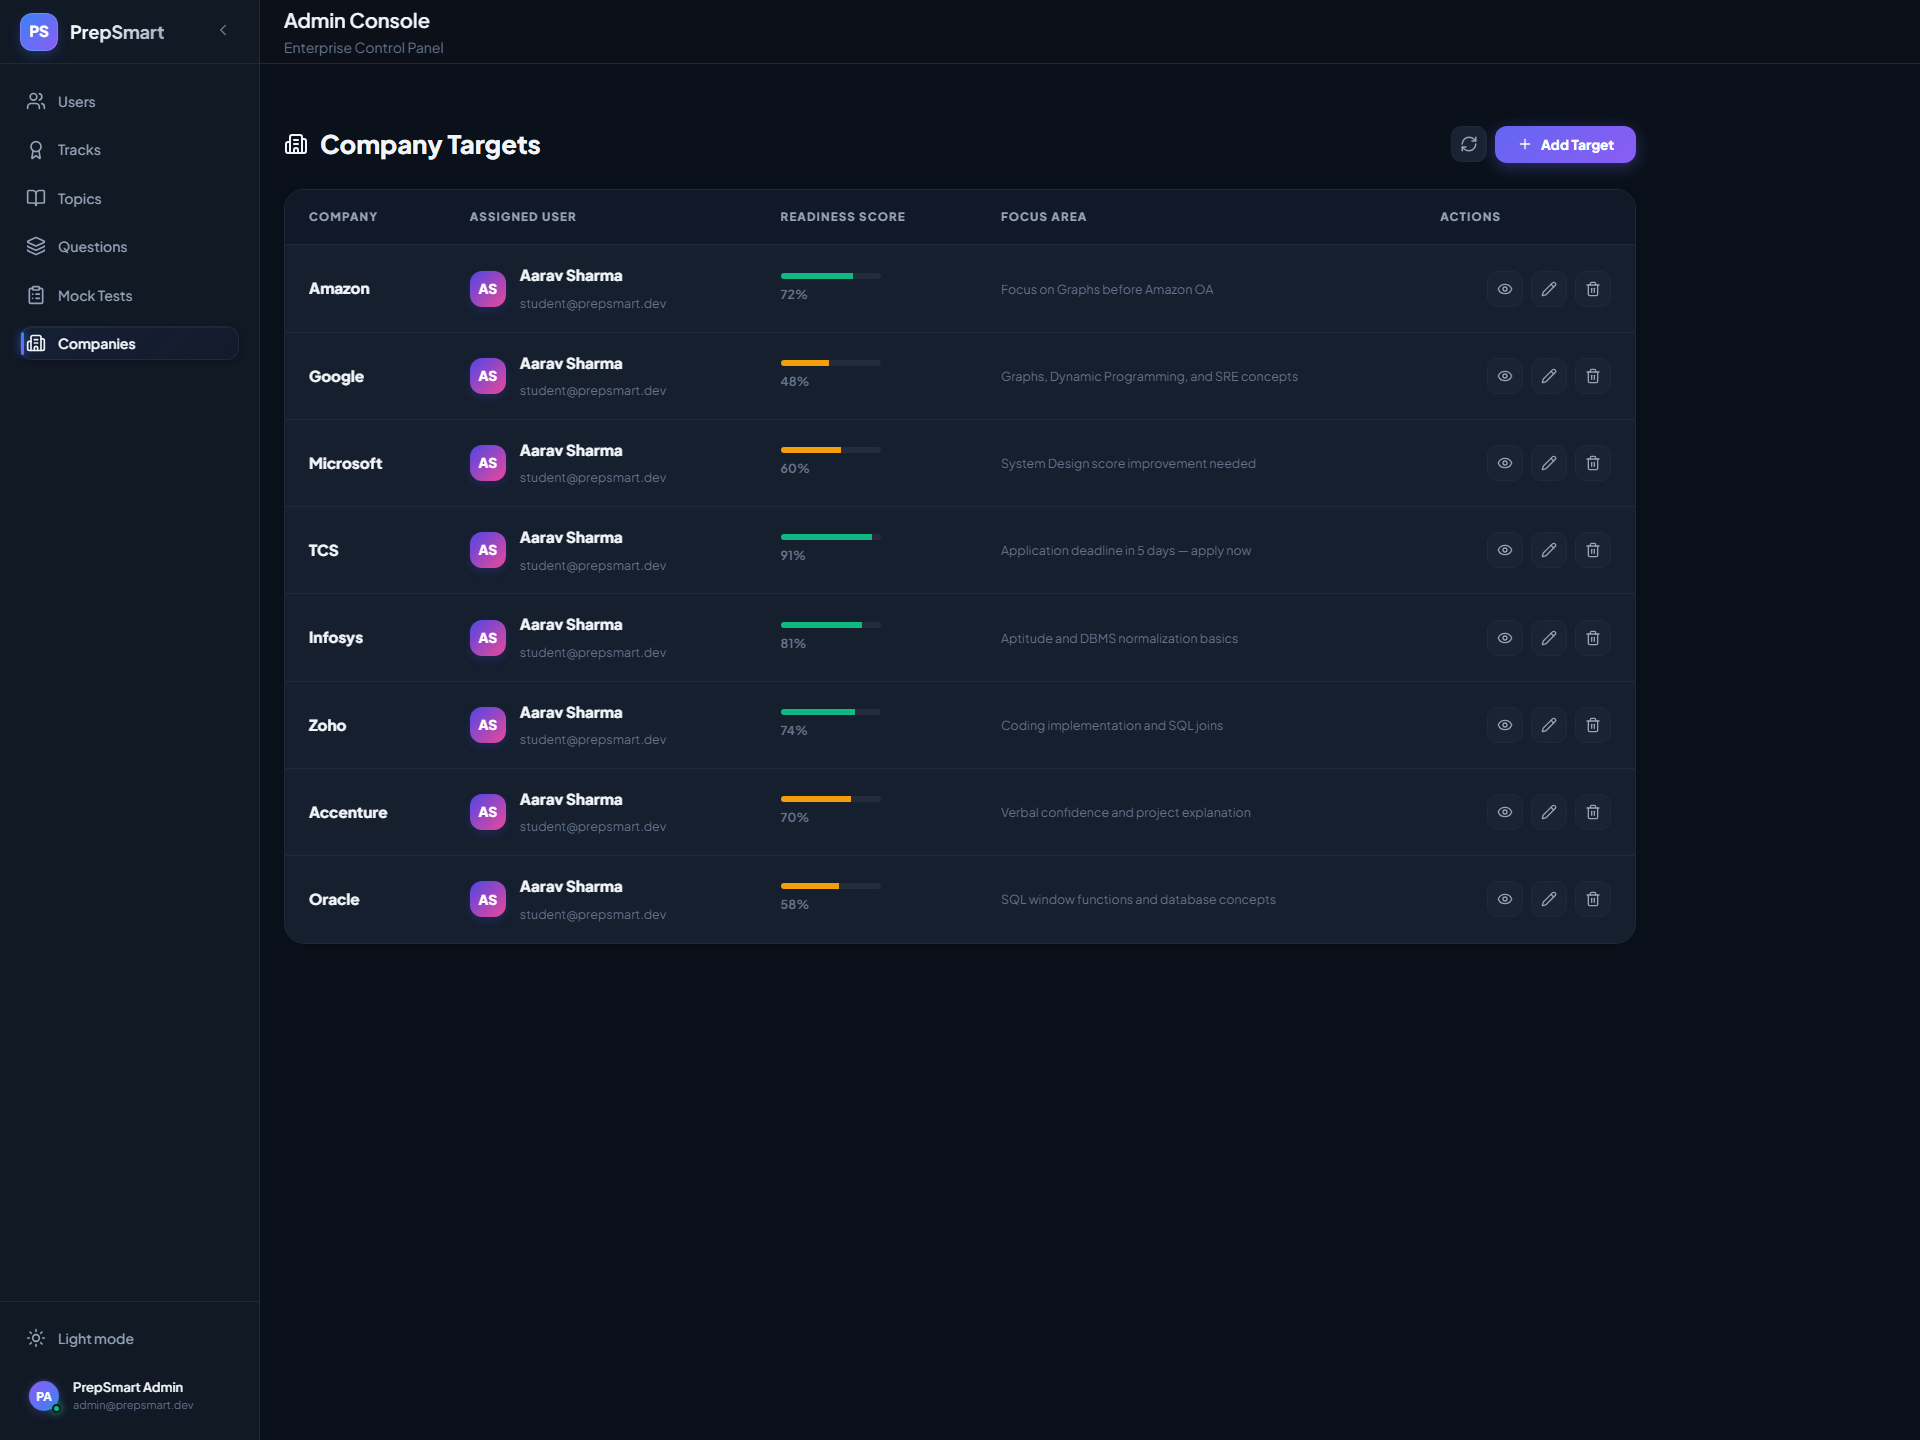
\includegraphics[width=0.90\textwidth]{Media/Chapter 5/admin_companies.png}
\caption{Administration - Company Management}
\label{fig:admin_companies}
\end{figure}

This interface enables administrators to maintain company-specific preparation information, readiness criteria, interview expectations, and recommended learning resources.

\subsection*{Major Features of the Administration Module}

\begin{itemize}

\item User account management.

\item Learning track administration.

\item Topic and content management.

\item Question bank maintenance.

\item Mock test administration.

\item Company information management.

\item Centralized platform administration.

\end{itemize}

\section{Chapter Summary}

This chapter presented the developed user interfaces of the PrepSmart platform and demonstrated the practical implementation of its major modules through screenshots. The chapter covered the landing page, user authentication, dashboard, placement preparation module, coding practice environment, AI interview module, company preparation module, profile management, shared profiles, analytics dashboard, settings, and administration module.

The presented interfaces demonstrate that PrepSmart successfully integrates multiple placement preparation activities into a single, user-friendly web application. The combination of modern user interface design, responsive layouts, real-time analytics, AI-assisted learning, and centralized management provides students with a comprehensive platform for effective placement preparation.

The next chapter discusses the overall conclusions of the project, summarizes the achieved objectives, identifies existing limitations, and presents possible directions for future enhancements.